
\documentclass[11pt]{report}
\pagestyle{myheadings}
\markright{Group 13\hfill FLAMeS \hfill}
\usepackage{pdflscape}
\usepackage{longtable}
\usepackage{multirow}
\usepackage{enumerate}
\usepackage[printonlyused]{acronym}
\usepackage{multirow}
\usepackage{graphicx}
\usepackage{wrapfig}
\usepackage{subfig}
\usepackage{amsmath}
\usepackage{url}
\usepackage{fixltx2e}
\usepackage{booktabs}
\usepackage{rotating}
\usepackage{bbding}
\usepackage{fancyhdr}
\usepackage{caption}
\usepackage{hyperref}
\hypersetup{pdfborder=0 0 0}

\topmargin -1.5cm
\oddsidemargin -0.04cm 
\evensidemargin -0.04cm 
\textwidth 16.59cm 
\textheight 21.94cm 
\parskip 7.2pt 

\pagestyle{fancy}

\renewcommand{\captionfont}{\footnotesize}
\renewcommand{\headrulewidth}{0 pt}

\begin{document}

\setcounter{secnumdepth}{5}
\setcounter{tocdepth}{2}
\pagenumbering{roman}

%%%%%%%%%%%%%
%
%       TOP MATTER
%
%%%%%%%%%%%%%

\begin{titlepage}
\begin{center}

\textsc{\LARGE Delft University of Technology}\\[1.5cm]

\textsc{\Huge Laser Swarm}\\[0.5cm]
\textsc{\small Final Report}\\[1.5cm]
\textsc{\large Design Synthesis Exercise}\\[2.5cm]

\begin{minipage}{0.4\textwidth}
\begin{flushleft} \large
\emph{Authors:}\\
\textsc{S. Billemont\\
L.S. Boersma\\
B. Buyens\\
S.R. Finck\\
J.P. Florijn\\
T.C. Goossens\\
N.S. Oborin\\
A.J. Vorobiev\\
G.J. van der Wel\\
Z. Zhou\\}
\end{flushleft}
\end{minipage}
\begin{minipage}{0.4\textwidth}
\begin{flushright}
\emph{Tutor:}\\
\textsc{Ben Gorte}\\[1cm]
\emph{Coaches:}\\
\textsc{Prem Sundaramoorthy\\
Mathieu Willaert}
\end{flushright}
\end{minipage}
\vfill

\today
\end{center}
\end{titlepage}

%%%%%%%%%%%%%
%
%       ABSTRACT
%
%%%%%%%%%%%%%

\normalsize
%\addcontentsline{toc}{chapter}{Abstract}
\begin{abstract}
Abstract text goes here
\end{abstract}

%%%%%%%%%%%%%
%
%       PREFACE
%
%%%%%%%%%%%%%

\chapter*{Preface}
\addcontentsline{toc}{chapter}{Preface}

The first month of this project has already passed, and this mid term report indicates and important milestone. We're not there yet, but we are getting on with it.

We did not, however, do everything by ourselves, and this is a good place to thank those who have been so kind as to give us some of their precious time.

First I want to mention professor Edoardo Charbon, who kindly explained and showed us the workings of his \ac{SPAD}\footnote{See \cite[98-105]{SPADThesis}, \cite{SPAD2} and \cite{SPAD3}}: without his help we would be hopelessly in the dark on these fascinating devices. From this place I also thank professor Kourosh Khoshelham for helping us to some valuable material on remote sensing. I also want to thank Jasper Bouwmeester, who provided us with some helpful information on solar panel pricing.

And finally I thank our tutor, professor Ben Gorte, who was very generous to us with his time and has been very supportive of the entire project.\\\\
I hope you will have as much fun reading this report, as we had in making it!\\\\
Yours sincerely,\\\\\\\\
 \hspace{2cm}Co Florijn,\\
 \hspace{2cm}Chairman

%%%%%%%%%%%%%
%
%       TOC
%
%%%%%%%%%%%%%
\footnotesize

\newpage
\phantomsection
\addcontentsline{toc}{chapter}{Contents}
\tableofcontents

\newpage
\phantomsection
\addcontentsline{toc}{chapter}{List of Figures}
\listoffigures

\newpage
\phantomsection
\addcontentsline{toc}{chapter}{List of Tables}
\listoftables

%%%%%%%%%%%%%
%
%       SYMBOLS
%
%%%%%%%%%%%%%

\newpage
\phantomsection
\addcontentsline{toc}{chapter}{List of Symbols}
\Large{\textbf{List of Symbols}}
\footnotesize
\begin{center}
\begin{longtable}{c|c|c}

\textbf{Symbol} & \textbf{Description} & \textbf{SI units} \\\hline\hline
A																		& prism apex angle																												& $^\circ$ \\

A																		& area 																																		& $m^2$ \\

a																		& semimajor axis 																													& km \\

a                                   & 

$A_{beam}$                    	    & laser beam area                               													& $cm^2$ \\

$A_Z$																& launch azimuth corrected for Earth's rotation  													& $^\circ$ \\

$A_{Z_I}$                           & launch azimuth in inertial reference frame  														& $^\circ$ \\

b                                  	& width                                       														& m \\

c                                   & speed of light                           																& $km/s$ \\

$C_D$																& drag coefficient 																												& $-$ \\

$C_{DD}$													  & diffuse drag coefficient																								& $-$ \\

$C_{DS}$						       					& specular drag coefficient 																							& $-$ \\

cg                                  & center of gravity                         															& m \\

$c_{pa}$                            & center of aerodynamic pressure            															& m \\

$c_{ps}$                            & center of solar pressure                   															& m \\

D																		& air drag 																																& N \\

D                                		& residual dipole of the satellite               													& $A.m^2$ \\

$d_{along}$                       	& along-track spacial resolution                  												& m \\

$d_{nadir}$                         & resolution in nadir direction                 													& m \\

E																		& electric field																													& - \\

$E_0$																& initial electric field																									& - \\

e 																	& eccentricity 																														& $-$ \\

$E_b$                               & received energy per bit                  																& J \\

$E_g$                               & energy gap                                 															& eV \\

$E_{p,damage}$                      & standard damage treshold energy            															& $J/cm^2/s$ \\

$f_{rep}$                     			& pulse repetition rate                   																& Hz \\

$F_S$                           		& solar constant                            															& $1367 W/m^2$ \\

G                                   & gravitational constant                      														& $6.67259\cdot 10^{-11} m^3/{kg.s^2}$ \\

g 																	& gravitational acceleration 																							& $m/s^2$ \\

H                                   & latitude shift                            															& km \\

h                                   & height                                      														& km \\

h                                   & Planck's constant                           														& J.s \\

$H_e$                               & reentry altitude     																										& km \\

$H_i$                               & initial altitude for deorbit manoeuvre     															& km \\

$I_{##}$                            & inertia tensor, $##$ indicates axis      																& $km.m^2$ \\

I                                   & signal attenuation                         															& dB \\

i 																	& inclination 																														& $^\circ$ \\

i                                   & incidence angle of the sun                 															& $^\circ$ \\

$I_{p,damage}$											& damage treshold intensity																								& $J/m^2$ \\

$i_R$ 															& relative inclination 																										& rad \\

$I_{sp}$													 	& specific impulse 																												& s \\

k																		& wave vector																															& - \\

L                                   & launch site latitude                        														& $^\circ$ \\

$L_x$                               & longitude shift                               													& km \\

M                                   & magnetic moment of the Earth                 														& $T.m^3$ \\

m 																	& mass 																																		& kg \\

$m_{dry}$                           & dry mass                                    														& kg \\

$m_{loaded}$												& sum of dry mass and propellant mass																			& kg \\

$m_{orbit}$                         & satellite mass once in orbit                														& kg \\

$m_propellant$ 											& propellant mass 																												& kg \\

$m_w$                               & reaction wheel mass  																										& kg \\

$m_{wd}$                            & mass of the reaction wheel disk  																				& kg \\

$m_{ws}$                            & mass of the reaction wheel skirt 																				& kg \\

$m_0$                               & dry mass                         																				& kg \\

N 																	& angular seperation 																											& rad \\

n 																	& index of refraction																											& $-$ \\

n                                		& angular velocity                             														& $deg/{min}$ \\

$n_e$ 															& refractive index 																												& $-$ \\

$N_0$                           		& noise density                                														& $W/Hz$ \\

P                             			& period                                      														& minutes \\

$P_{continuous}$ 										& power of a continuous laser beam																				& Watt \\

$P_{output}$                       	& output power                             																& Watt \\

$P_{pulsed}$ 												& power of a pulsed laser beam																						& Watt \\

PSD                             		& power spectral density                       														& $g/{Hz^2}$ \\

q                               		& reflectance ratio                              													& - \\

R																		& radius of the orbit of the center of mass 															& km \\

r                                   & radius                                                                  & m \\

T 																	& temperature 																														& K \\

$T_a$                             	& aerodynamic disturbance                         												& N.m \\

$T_e$                              	& eclipse time                             																& minutes \\

$T_g$                         			& Earth's gravity gradient                        												& N.m \\

$t_{lens}$													& lens induced phase difference																						& rad \\

$T_m$                         			& disturbance of the Earth's magnetic field     													& N.m \\

$t_p$                          			& pulse time                         																			& seconds \\

$T_{sp}$                        		& solar radiation disturbance                 														& N.m \\

$T_{\omega}$                       	& torque                                 																	& N.m \\

V																		& velocity																																& m/s \\

$V_a$ 															& bias supply voltage 																										& V \\

$V_b$ 															& breakdown voltage																												& V \\

$V_e$ 															& excess bias voltage																											& V \\

$V_{eq}$                            & velocity of Earth's rotation at the equator 														& $m/s$ \\

$V_i$                               & initial orbital velocity      																					& $m/s$ \\

$V_L$                               & inertial velocity of the launch site        														& $m/s$ \\

$v_0$                               & launcher orbital velocity before spearation 														& $m/s$ \\

w																		& beam waist																															& m \\

$w_0$                       				& initial beam waist                                      								& m \\

z                             			& zenith angle                                  													& $^\circ$ \\     
 
$\alpha$                            & relative inclination                        														& $^\circ$ \\

$\alpha$                            & incidence angle                        																	& $^\circ$ \\

$\alpha$                            & induced divergence                       																& $^\circ$ \\

$\gamma$                            & divergence angle                         																& $^\circ$ \\

$\Delta N$                          & angular seperation at ascending nodes            												& $^\circ$ \\   

$\Delta V$                          & change in speed required for different orbit 														& $m/s$ \\

$\Delta V_{deorbit}$                & change in speed required for deorbit and reentry  											& $m/s$ \\ 

$\Delta V_{planechange}$            & change in speed required for the correction of injection inaccuracy			& $m/s$ \\ 

$\epsilon$                         	& deviation angle                          																& $^\circ$ \\

$\eta$ 															& nadir angle																															& $^\circ$ \\

$\eta_{wp}$                       	& electrical to optical power efficiency of a laser system  							& - \\

$\theta$                            & natural optical Gaussian beam divergence       													& $^\circ$ \\

$\theta$                            & deviation from nadir                             												&  $^\circ$ \\

$\Theta$                            & Henyeye-Greenstein term                           											& rad \\

$\kappa$                            & Minnaert parameter                  																		& - \\

$\lambda$ 													& wavelength																															& m \\

$\lambda$ 													& seperation angle																												& $^\circ$ \\ 

$\mu$														 		& gravitational constant of the Earth 																		& $398600\cdot 10^9$ $m^3/s^2$ \\

$\rho$ 															& density 																																& $kg/m^3$ \\

$\phi$ 															& phase angle 																														& rad \\
	
$\phi _R$														& relative phase angle 																										& rad \\

$\psi$															& phase difference																												& rad \\
     
$\Omega$ 														& right ascension of the ascending node 																	& rad \\

$\omega$ 														& argument of perigee																											& rad \\

$\omega_{drift}$                    & drift rate                                  														& $^\circ/orbit$ \\

$\dot \omega$ 											& time rate of change of the argument of perigee 													& rad/s \\

$\dot \Omega _{J_2 }$ 							& rate of precession 																											& rad/s \\

$\dot \omega_{max}$                 & maximum angular acceleration                														& $rad/s^2$ \\ 
 
\end{longtable}
\end{center}

%%%%%%%%%%%%%
%
%       ACRONYMS 
%
%%%%%%%%%%%%%

\newpage
\phantomsection
\addcontentsline{toc}{chapter}{List of Acronyms}
\Large{\textbf{List of Acronyms}}
\footnotesize
% ALPHABETIZE!!!
\begin{acronym}[LiDAR]
\acro{ADCS}{Attitude Determination and Control Subsystem}
\acro{BLR}{Base Line Review}
\acro{CCD}{Charge-Coupled Device}
\acro{CMG}{Control Moment Gyro}
\acro{EIRP}{Effective Isotropic Radiated Power}
\acro{EOL}{End-of-life}
\acro{EPS}{Electrical Power System}
\acro{FBS}{Functional Breakdown Structure}
\acro{FFD}{Functional Flow Diagram}
\acro{FR}{Final Review}
\acro{G/T}{Receiver antenna gain / receiver system noise temperature}
\acro{GEO}{Geosynchronous Earth Orbit}
\acro{GLAS}{Geoscience Laser Altimeter System}
\acro{GSE}{Ground Support Equipment}
\acro{HEllO}{Highly Elliptical Orbit}
\acro{HEO}{High Earth Orbit}
\acro{IAT}{Integration, Assembly and Test}
\acro{laser}{Light Amplification by Stimulated Emission of Radiation}
\acro{LEO}{Low Earth Orbit}
\acro{LiDAR}{Light Detection And Ranging}
\acro{LOOS}{Launch and Orbital Operations Support}
\acro{LPA}{Laser Profiling Array}
\acro{MEO}{Medium Earth Orbit}
\acro{MNS}{Mission Need Statement}
\acro{MTR}{Mid Term Review}
\acro{OFOV}{Optical Field of View}
\acro{OM}{Operations and Management}
\acro{ORD}{Optical Receiving Device}
\acro{POS}{Project Objective Statement} 
\acro{QDRD}{Quantum Dot Receiving Device}
\acro{RAMS}{Reliability, Availability, Maintainability and Safety}
\acro{RDTE}{Research, Development, Test and Evaluation}
\acro{SLR}{Satellite Laser Ranging}
\acro{TDRS}{Tracking and Data Relay Satellite}
\acro{TFU}{Theoretical First Unit}
\acro{TRL}{Technology Readiness Level}
\acro{TT\&C}{Telemetry, Tracking and Command}
\end{acronym}
\small

%%%%%%%%%%%%%
%
%       INTRODUCTION
%
%%%%%%%%%%%%%
\chapter{Introduction}
\label{chap:intro}
\pagenumbering{arabic}
In February 2010 the ICESat mission ended after 7 years of measuring ice sheet mass balance, cloud and aerosol heights, as well as land topography and vegetation characteristics.
To do all this, ICESat had only one instrument on board: a space based \ac{LiDAR} system (\ac{GLAS}), allowing for an unprecedented 3D view of the Earth's surface and atmosphere.
The laser lifetimes, however, were severely limited because of manufacturing errors in one of the laser components.

ICESat followed only one of the possible approaches for \ac{LiDAR}, namely the use of a high energy laser and a large receiver telescope. The other approach is using a high frequency low energy laser and a single photon detector. The advantage of the latter approach is that it has a much lower mass, but it is uncertain if even a single photon per pulse reaches the receiver. One possible solution could be the use of a swarm of satellites around the emitter, each equipped with a single photon detector. However the technical feasibility of this concept has not yet been proven.

In this mid term review some options for this concept are proposed and traded off so as to find the best fit for the mission. This tradeoff is what the bulk of this report is about. Also described are the workings and results from the simulator, as well as the project and risk management. Chapters on operation and logistics, stability and control and sustainability are included too.

% Chapter \ref{blFuncChapter} describes the functions and requirements of the system as a whole, whereas Chapter \ref{blBudgets} shows the multiple budget breakdowns and resource allocation. In Chapter \ref{blRisk} the technical risks are investigated. Chapter \ref{blDesignOptions} illustrates the different design options. Since sustainable engineering is an important factor, Chapter \ref{blSustainable} is devoted to this subject. In Chapter \ref{blInvestment} the return on investment and operational profit are discussed and finally in Chapter \ref{blRAMS1} the \ac{RAMS} are studied.

\rhead{\setlength{\unitlength}{1cm}
\begin{picture}(0,0)
\put(-1,-0.7){\includegraphics[width = 2cm]{anim/pic\thepage.png}}
\end{picture}}
%%%%%%%%%%%%%
%
%	 Project Management
%
%%%%%%%%%%%%%

\chapter{Project Management}
\label{chap:project_management}
The correct management of a project is very important because modern projects are extremely multidisciplined. Therefore it is easy to descend into chaos if no proper project management is applied. Thus it is necessary to devote a chapter of the report to the project management.
\\\\
One way to maximize efficiency is to make sure that everybody has a clear cut task. Therefore a resource allocation was performed. The results can be ssen in section \ref{DDHR}. Budget breakdowns are a good tool to know the total budgets in terms of mass, cost and power. When these are made it is easy to quickly check up and see what the mass, cost or power usage of each component is. The individual breakdowns are given in sections \ref{DDMBB}, \ref{DDCB} for the cost and maas budget breakdown. The power usage breakdown for the emitter can be found in section \ref{emitter_EPS} and that for the receiver in section \ref{receiver_EPS}.
Section \ref{OperationsLogistics} discusses the operation and logistic aspect of the mission in detail.
The mission lifetime extends far beyond these ten weeks. The timeline of this mission can be seen in the Gantt chart in section \ref{frPMgantt}.
\section{Human Resource Allocation}
\label{DDHR}
The first part of the project will involve a team of five specialists designing the five critical subsystems and one person designing the orbits of the swarm. The other four members will concentrate on the development of the software that will be used to assist the trade-off and verify the design. At later stages, some of the the software engineering personnel is heavily involved in designing proper algorithms for the processing of mission data, while others will be brought in to assist with detailed design. 

A schematic representation of the resource allocation can be found in figure \ref{fig:DDBBHR} on page \pageref{fig:DDBBHR}.

\begin{figure}[h!]
\begin{center}
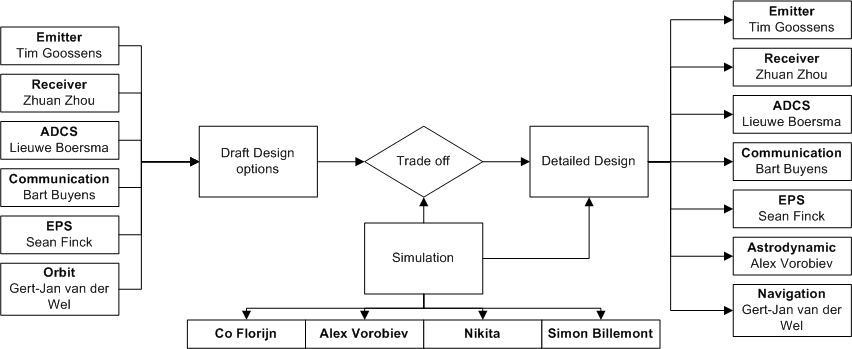
\includegraphics[width=0.9\textwidth]{chapters/img/DDBBHR.jpg}
\end{center}
\caption{Human resource allocation chart.}
\label{fig:DDBBHR}
\end{figure}

Table \ref{tab:RWD} on page \pageref{tab:RWD} indicates the allocation of tasks to each person.

\newpage
\begin{center}
\begin{longtable}{|l|l|c|c|}\hline
 Chapter & Documentation                      & Author & Checked by \\\hline\hline
 -       & Title Page                           & Alex & - \\\hline     -       & Abstract                             & Lieuwe & \\\hline    
 -       & Preface                              & Co, Team& All \\\hline
 -       & List of Symbol                       & Sean & - \\\hline\hline
 1       & Introduction                         & Bart &\\\hline\hline
 2       & Project Management                   & - & -\\\hline
 2.1     & \ -Human Resource Allocation         & Zhuan & Sean, Nikita \\\hline
 2.2     & \ -Operations and Logistic Concept Description & GJ & Bart \\\hline
 2.3     & \ -Project Design and Development Logic & Lieuwe & Sean, Nikita \\\hline
 2.4     & \ -Project Gantt Chart               & Lieuwe & Nikita \\\hline\hline
 3       & Mission Approach                     & - & -\\\hline
 3.1     & \ -Function Flow Diagram             & Lieuwe, Zhuan & Bart \\\hline
 3.2     & \ -Function Breakdown Structure      & Lieuwe, Zhuan & Bart \\\hline
 3.3     & \ -H/W Block Diagram                 & Lieuwe, & GJ \\\hline
 3.4     & \ -S/W Block Diagram                 & Nikita & GJ \\\hline
 3.5     & \ -Electrical Block Diagram          & Sean & Bart \\\hline
 3.6     & \ -Data Handling Block Diagram       & GJ & Bart\\\hline
 3.7     & \ -Communication Block Diagram       & Bart & GJ\\\hline
 3.8     & \ -Mass Budget Breakdown             & Zhuan & Sean, Nikita \\\hline
 3.9     & \ -Cost Budget Breakdown             & Zhuan & Sean, Nikita \\\hline\hline
 4       & Risk Management                      & Tim, Zhuan & GJ \\\hline\hline
 5       & Launch and Astrodynamic Characteristics & Alex & -\\\hline
 5.1     & \ -Launch Segment                    & Alex, Sean & Co \\\hline
 5.2     & \ -Space Segment                     & Alex & Co \\\hline
 5.3     & \ -Space Environment and Shielding   & Alex & Co \\\hline\hline
 6       & Emitter Satellite                    & - & -\\\hline
 6.1     & \ -Detailed Design Optical Emitting Payload & Tim & Sean, Co \\\hline
 6.1.1   & \ \ -Principle of AlGaAs Laser Diode & Tim & Sean, Co \\\hline
 6.1.2   & \ \ -Diode Pumped Solide-State Laser Configuration & Tim & Sean, Co \\\hline
 6.1.3   & \ \ -Optical Characteristics        & Tim & Sean, Co\\\hline
 6.1.4   & \ \ -Gaussian Beam Propagation and Diffraction & Tim &  Sean, Co\\\hline  
 6.1.5   & \ \ -Thermal Control                & Tim, Lieuwe & Sean, Co\\\hline
 6.1.6   & \ \ -Laser Lifetime Expectancy     & Tim & Sean, Co\\\hline
 6.1.7   & \ \ -Laser Focus Calculation        & Zhuan & Sean, Co\\\hline
 6.2     & \ -Navigation                        & GJ & Sean \\\hline
 6.3     & \ -Communication Subsystem           & Bart & Sean\\\hline
 6.4     & \ -ADCS                              & Lieuwe & Sean\\\hline
 6.5     & \ -EPS                               & Sean & Nikita\\\hline\hline
 7       & Receiver Satellite                   & - & - \\\hline
 7.1     & \ -Detailed Design Optical Receiver Payload & Zhuan, Co & Nikita, Co\\\hline
 7.1.1   & \ \ -SPAD                           & Tim, Zhuan & Nikita, Co\\\hline
 7.1.2   & \ \ -Prism Design                   & Zhuan & Nikita, Co\\\hline
 7.1.3   & \ \ -Summary                        & Zhuan & Nikita, Co\\\hline
 7.1.4   & \ \ -Payload Cost Estimation        & Tim, Zhuan & Nikita, Co\\\hline
 7.2   & \ -Navigation                        & GJ & Nikita\\\hline
 7.3     & \ -Communication Subsystem           & Bart & Nikita\\\hline
 7.4     & \ -ADCS                              & Lieuwe & Nikita\\\hline
 7.5     & \ -EPS                               & Sean & Nikita\\\hline\hline
 8       & Data Validation                      & Simon, Co, Nikita & Nikita \\\hline
 8.1     & \ -Software Tool Internals           & Simon, Co, Nikita & Nikita \\\hline
 8.2     & \ -Validation Results                & Simon, Co, Nikita & Nikita \\\hline\hline
 9       & Sustainable Development Strategy     &Bart, Sean & \\\hline\hline
 10      & Compliance Matrix                    & Sean & GJ \\\hline\hline
 11      & Conclusion and Recommendations       & lieuwe &\\\hline\hline
 -       & Others                               & - & - \\\hline
 -       & \ -Catia Drawing                     & Lieuwe & -\\\hline
 -       & \ -Latex Compile                     & Zhuan & -\\\hline

\caption{Report writing distribution.}
\label{tab:RWD}
\end{longtable}
\end{center}
\chapter{Operations and Logistics}
\label{OperationsLogistics}

In order for the laser swarm to be successful it has to operate efficiently and effectively, so that the obtained surface model and other data can be sold on the market. This chapter will consider some of these operations and their required logistics. Note that only operations after successful orbit injection and deployment, and before the \ac{EOL} are considered. A graphical representation of the hierarchy of the options considered here can be found in figure \ref{fig:OpsHier} on page \pageref{fig:OpsHier}.

\begin{figure}
\centering
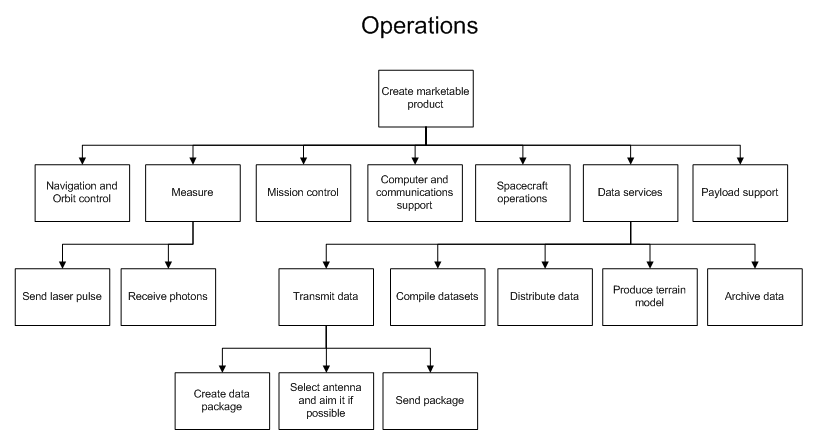
\includegraphics[width=1.0\textwidth, angle=0]{img/OpsHierarchy.png}
\caption{Hierarchy of the operations for the laser swarm mission.}
\label{fig:OpsHier}
\end{figure}

Navigation and orbital control is an important operation for the laser swarm mission. For example, without an accurate knowledge of the position of the satellites the gathered data is useless and orbital control cannot be performed. All satellites use a \acs{GPS} receiver to determine their position up to about one meter. Orbital control is performed automatically based on the received \acs{GPS} data. It is clear by now that this system is to work automatically, however it is important there are people on the ground who check for any anomalies and give corrections whenever necessary.

Mission control entails the real time control of the satellites. However because the mission is automated the amount of people for mission control can be limited. The only active inputs by humans are commands sent to the satellite to correct for any errors that may occur.

The measurements will be performed completely autonomously, with human inputs only being used to correct an error in the automation or to change the mission routine. The measuring operation includes the both the emitter and the receivers, for a greater detail of the functions that have to be performed the function flow diagram in section \ref{section_FFD} may be consulted.

Payload support is comprised of one or more people who monitor the condition and performance of the laser payload, and a separate group of people who monitor the receiving payload on both the emitter and receiver satellites. In case of an anomaly they determine the severity and adjust the payload operations or satellite functioning to correct the problem.

Spacecraft operations is similar to payload support, except that the person or people who work on this operation monitor the other subsystems of the satellite by analyzing the housekeeping data from the payloads, navigational systems, the power subsystems or the antennae to name some examples.

Computer and communications support has a staff of several people who monitor the onboard computer of the satellites and the system automation, and one or two persons who monitor the communications between satellites and from the emitter satellite to the ground. Their main job is to ensure the system remains operational if an anomaly occurs.

Data services entails everything that happens with all data both on ground and aboard the satellites. The data can be anything from measurement data to navigational data and housekeeping data. This operation supports all others. While largely automated some human interaction is needed to ensure the data in decoded, debugged, archived and generally handled properly. Minimal human interaction should be required to reduce the mission costs.

Data transmission involves the sending of data between satellites and from the satellites to a ground station. The satellites will use their position and attitude data to determine which antenna to use for intersatellite communication, and the emitter will perform a similar operation using its own position and attitude data direct communications to the ground station. This process is fully automated, and a failure in the X-band phased array means that a ground station will have to aim towards a receiver satellite in order to attempt to fix the problem. So normally this operation requires no personnel, but in case of failure several persons are required to attempt to save the mission.
\section{Project Design and Development Logic}
\label{frPMgantt}
Since the \ac{FLAMeS} mission is an earth observation mission the main stakeholders are researchers and the scientific community. They are the main drivers for the requirements of the mission. It is the challenge for the project engineers to translate those requirements into a working satellite system. One of the key features of the mission is to use a formation of mostly identical satellites, which eases the mission development and design compared to a mission with nine unique satellites. 

Both types of satellites can be developed in parallel, since apart from the receiver instrument and the communication link the satellite designs are completely independent of each other. The fact that the design of the receiver satellites is based on the cubesat standard will reduce the time of the development considerably, since a lot of technology and components are standardised and available off the shelf. The testing equipment and infrastructure can be reused and will not have to be custom-made for every single satellite in the formation. 

Most of the basic satellite components used for the design of the emitter satellite are \ac{COTS} as well, which shortens the development and qualification time for that satellite. Most of the development time and cost will have to be put into the detailed design of the payloads, which are specialised instruments dedicated to this mission. Another critical part of the mission is the redesign of the rocket's upper stage to make it able to put all satellites in their own orbit.

A fast development time saves resources and will enable the mission to be launched in the spring of 2017. This way the measurements can be made at solar minimum and the least amount of propellant is needed for station keeping and orbital manoeuvres.

\section{Project Gantt Chart}
Naturally the \ac{FLAMeS} mission will extend a lot further in time than just the this feasibility study. To keep the mission on track until and beyond the launch a Gantt chart is set up for the project.

After the feasibility study is finished the precise mission definition is performed. When the exact requirements for all subsystems are known the detailed design can start. As soon as the design is fixed for different subsystems production and assembly of the subsystems can start. Even while the production is still in progress the acceptance testing of the finished components and representative mock-ups can take place. This way design mistakes or production errors can be discovered early and problematic parts can be fixed or even redesigned. When all parts are finalised and tested the satellite can be integrated and transported to the launch site. When the satellite is put on the launcher the launch can commence.

After launch first the satellites need to be put in their correct orbits and the instruments are calibrated. Then the real mission can start and measurements are made. As soon as data is collected and send to the ground, researchers can start analysing the data and producing and publishing results. 

The Gantt chart can be found in figure \ref{ganttchart} on page \pageref{ganttchart}.

\begin{figure}
\centering
%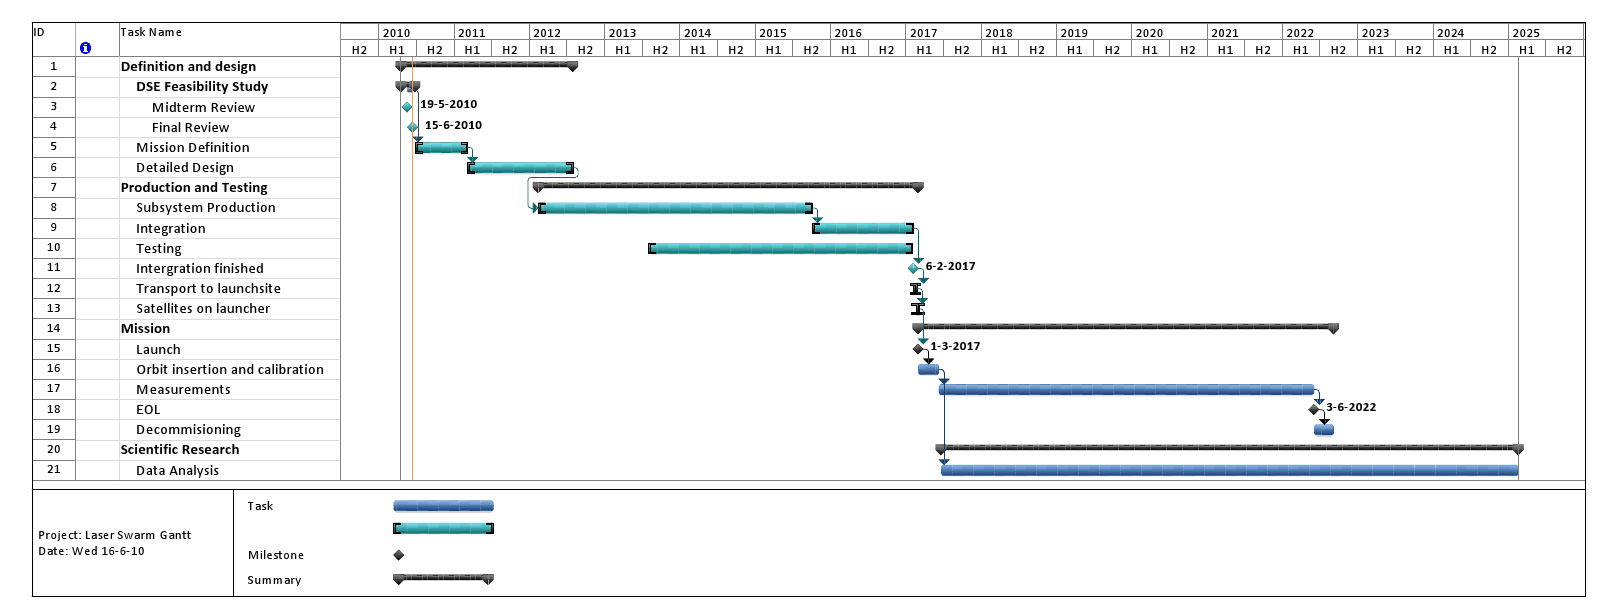
\includegraphics[width=0.8\textwidth, angle=90]{chapters/img/projectganttchart.png}
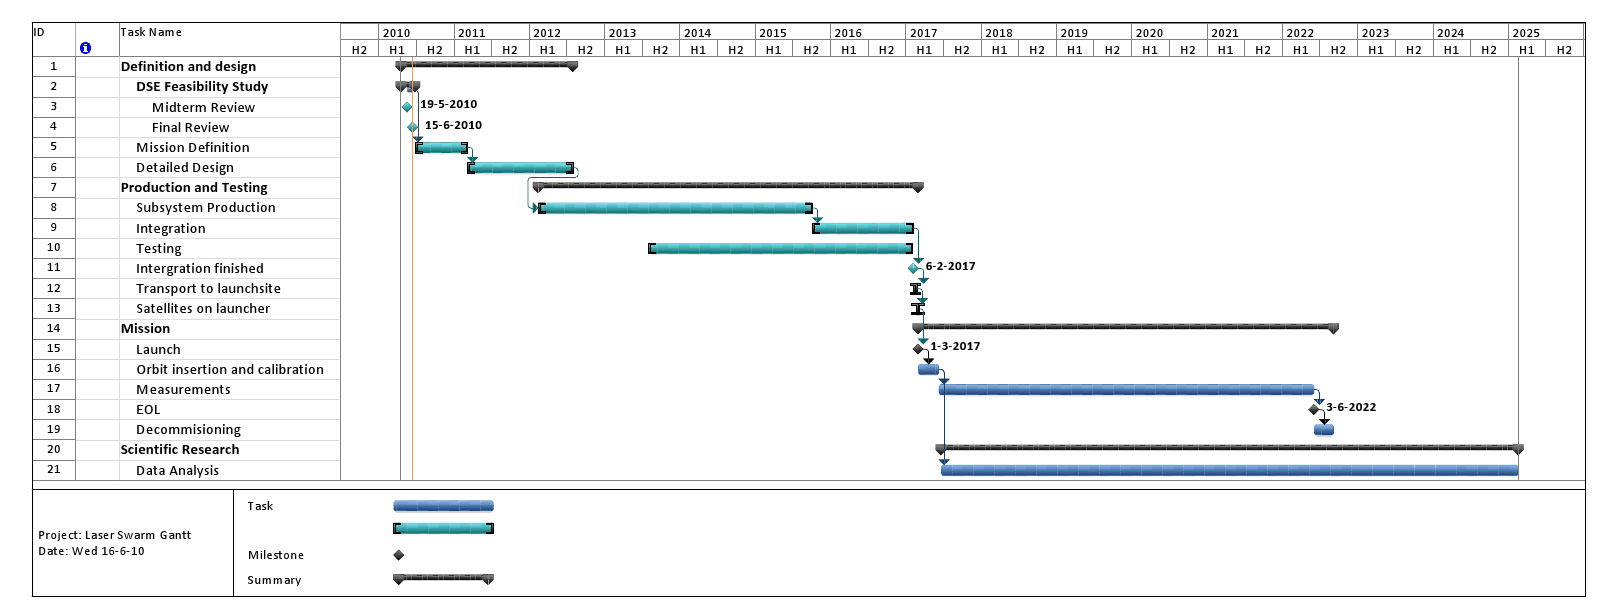
\includegraphics[width=1.2\textwidth, angle=90]{chapters/img/projectganttchart.png}
\caption{Project Gantt Chart}
\label{ganttchart}
\end{figure}

%%%%%%%%%%%%%
%
%	 Mission Approach
%
%%%%%%%%%%%%%

\chapter{Mission Approach}
\label{chap:mission_approach}
\label{MissionApproachIntro}

The \ac{FLAMeS} mission consists of nine satellites in six different orbits, these satellites consist of two types. The first is called the emitter satellite, because it carries the laser payload (emitting payload). The second type is the receiver satellites, earning the name by only have a receiving payload. Unless clarity poses a problem these satellites a referred to as simply the emitter and receiver.

This chapter will show a function overview of the mission and how different systems of the satellite cooperate to ensure a successful mission. First the functional flow diagram is discussed in section \ref{section_FFD} and the functional breakdown structure follows in section \ref{section_FBS} on page \pageref{section_FBS}. After that the hardware block diagram and software block diagram are discussed in section \ref{H/W Block Diagram} on page \pageref{H/W Block Diagram} and section \ref{section_SWBD} on page \pageref{section_SWBD} respectively. Section \ref{EBD} shortly discusses the electrical block diagram and section \ref{DHBD} on page \pageref{DHBD} handles the data handling block diagram for the emitter satellite and the receiver satellite. The final part of this chapter treats the communications flow diagram on page \pageref{CFD} in section \ref{CFD}.
\section{Functional Flow Diagram}
\label{section_FFD}
The \ac{FFD} shows the functions the system needs to perform during its mission life. The schematic representation is divided into 2 parts. Part 1 detailed top level functions F1 and F2 (Figure \ref{FFD1} on page \pageref{FFD1}) meanwhile part 2 detailed top level functions F3, F4 and F5 (Figure \ref{FFD2} on page \pageref{FFD2}).

The first thing that needs to happen, after having been built, is that the satellites are put into their orbits and pointed towards earth. After that the measurements can start: the emitter sends down laser pulses and notifies the receivers that the signals are sent. The receivers can adjust their attitude, pick up reflected photons, turn them into a digital signal and inform the computer, which puts the data in a buffer. The data of the receivers will be sent to the emitter satellite continually and then it will transfer the data package to ground when the emitter is passing the ground station. The data on the ground can be split up into data packages, which can be distributed to research institutes and other interested parties. With those data sets, a terrain model and \ac{BRDF} can be recreated. At the \ac{EOL} of the mission the satellites are decommissioned to make room for other satellites.

\begin{landscape}
\begin{figure}[ht!]
\centering
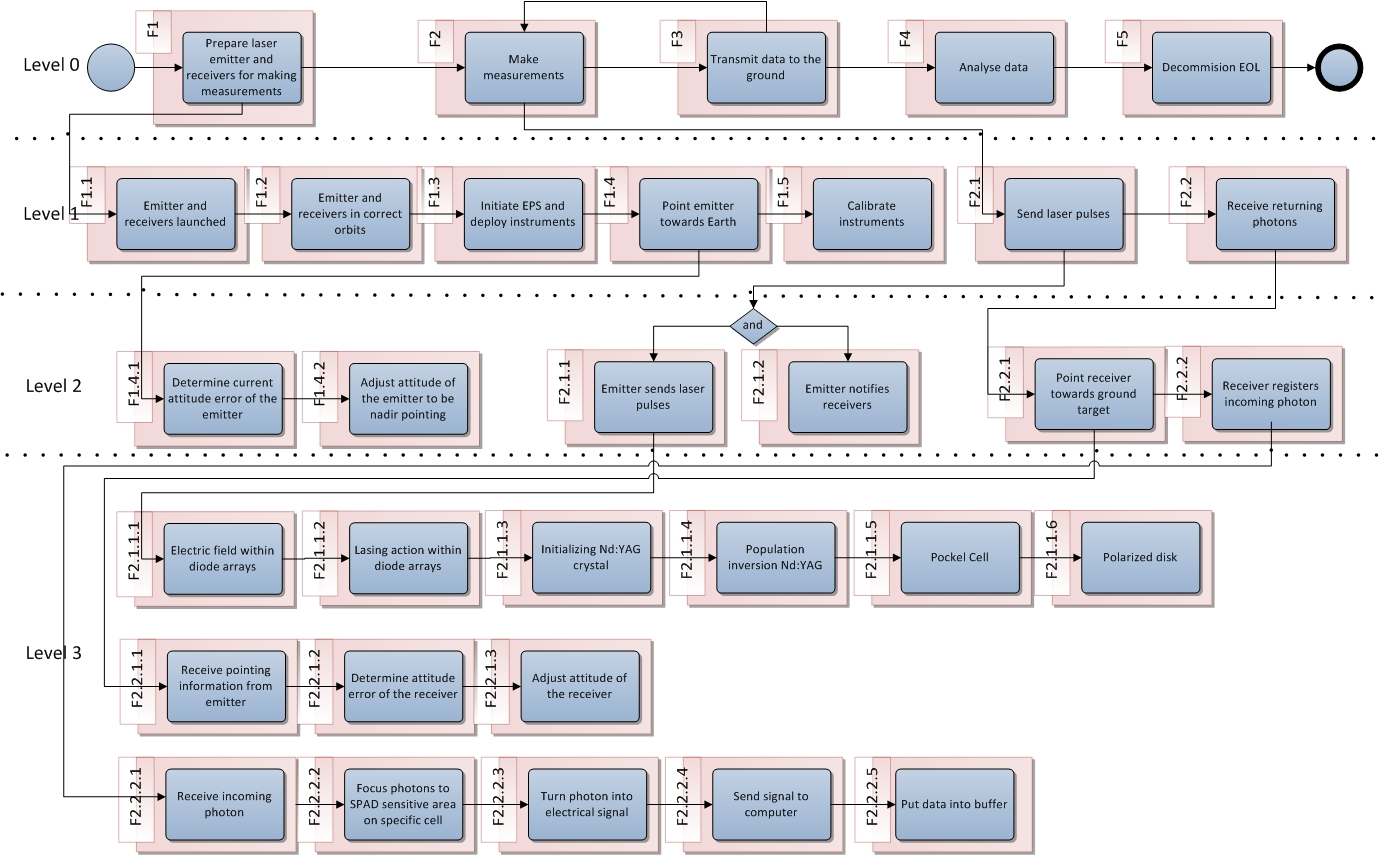
\includegraphics[width=1.3\textheight]{chapters/img/FFD1.jpg}
\caption{Functional Flow Diagram part 1(F1 and F2 detail) of the Laser Swarm mission}
\label{FFD1}
\end{figure}
\end{landscape}

\begin{landscape}
\begin{figure}[ht!]
\centering
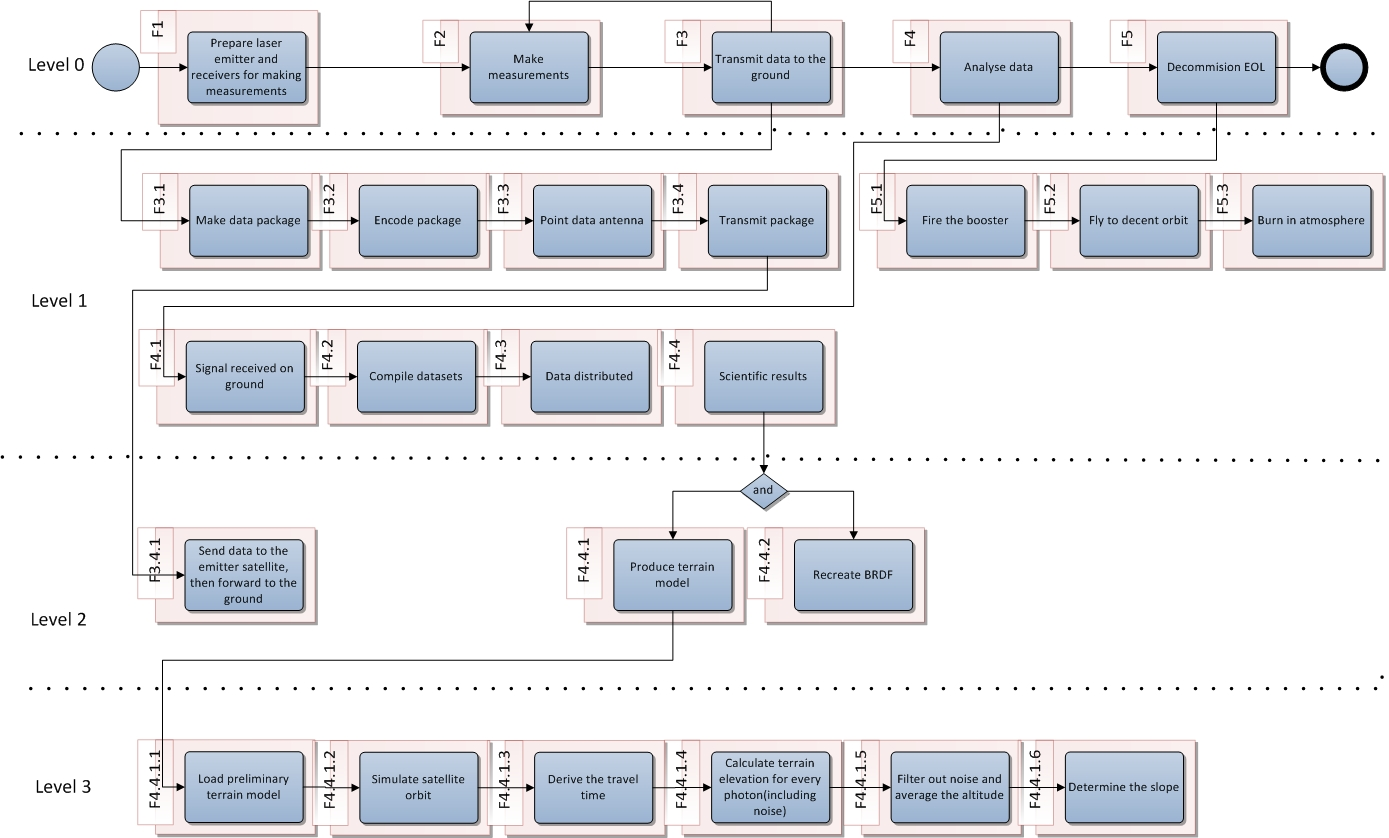
\includegraphics[width=1.3\textheight]{chapters/img/FFD2.jpg}
\caption{Functional Flow Diagram part 2(F3, F4 and F5 detail) of the Laser Swarm mission}
\label{FFD2}
\end{figure}
\end{landscape}

\section{Functional Breakdown Structure}
\label{section_FBS}
The \ac{FBS} shows the functions the system needs to perform, broken up in subtasks from other functions. The schematic representation can be found in figure \ref{FBS} on page \pageref{FBS}.

\begin{landscape}
\begin{figure}[ht!]
\centering
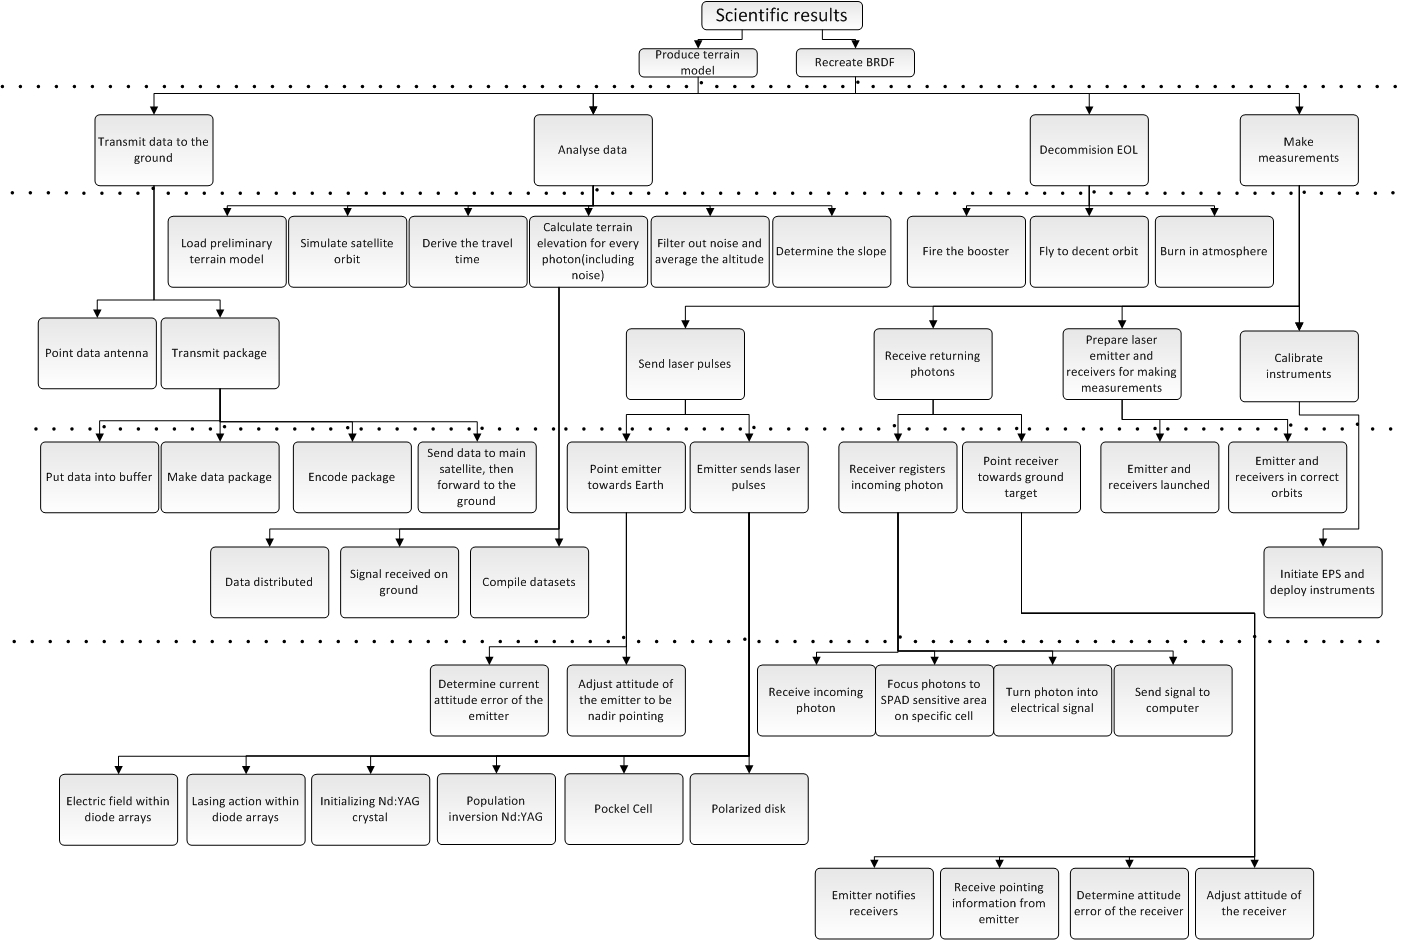
\includegraphics[width=1.3\textheight]{chapters/img/FBD.jpg}
\caption{Functional breakdown structure of the Laser Swarm mission}
\label{FBS}
\end{figure}
\end{landscape}

The main function for the system is to be able to get scientific results as producing terrain model and recreating \acs{BRDF}, which is the reason for making the measurements. To be able to produce the terrain model the measurements need to be made, the data needs to be transferred to the ground and the data needs to be analyzed. Because the mission has to be sustainable, the satellites are decommissioned at the end of their life, so they will not pose a threat to other satellites in the same orbit.

The measurements depend on laser pulses to be sent, returning photons to be detected and for the emitter and receivers to be in orbit with the instruments calibrated. For the data to be transmitted to Earth, the antenna needs to be pointed to the ground station and the data package has to be transmitted. Data analysis depends on the data to be received on the ground and the distribution between the research institutes.

To have the satellite send out laser pulses the satellite needs to point down (nadir-pointing) and the emitter needs to send the pulses. Receiving photons depends on the receiver being pointed at the ground target and the receiver is able to register incoming photons. For the data package to be transmitted, data is put into a buffer, a data package is made, the package is coded and the receiver sends the data to the emitter satellite, which in turn forwards it to Earth. It is important to have the \ac{EPS} properly functioning and instruments deployed before they can be calibrated.

Determining the attitude error of the emitter and adjusting the it accordingly is required to point the emitter towards Earth. When an incoming photon is received, it is transformed into a digital signal and the signal is sent to the on-board computer so the photon is registered. For the receiver to be pointed at the ground target, the emitter needs to notify the receiver it has sent pulses. The receiver needs to receive the message, interpret it, determine attitude error and adapt accordingly to make sure that data gathering will be carried out properly. 





\section{H/W Block Diagram}
The hardware block diagram shows the interactions between the different components of the subsystems of the satellites. The diagram is split in two parts, a part for the emitter and one for the receiver. Most systems are the same for both the emitter and receiver satellites. The main differences are in the payload and the communication subsystems.

The "heart" of the satellites is the \ac{CDH} subsystem with the On-board Computer and the Data Handling and Storage. All data goes through this subsystem and is sent to other subsystems for which it is relevant. 

Most subsystems require power to function, so everything is linked to the \ac{EPS} as well. In the diagrams these lines are left out the diagram, so the diagrams is readable. Striped blocks do not require power. The solar panel pointing mechanism points the solar panels towards the Sun during the day (Sunlit) phase, the solar panels supply their power to the power regulator and the batteries. During the night (eclipse) phase the batteries provide power to the power regulator. The regulator distributes the power to the different subsystems.

The \ac{ADS} determines the attitude of the satellite, using the sun sensors during the day and with the star tracker during the night, and sends it to the \ac{CDH}. If there in an error in the attitude, the \ac{ACS} can adjust for that after it is being told to. Before the reaction wheels are saturated the magneto torquers can be used to desaturate them. The Navigation part of the Communications subsystem determines the orbit and position of the satellites. The thruster can make orbit changes if necessary.

The link between the satellites uses a high-high S-band patch antenna. The data link from the emitter to the ground is done with an X-band antenna array. Each satellite also is equipped with a nadir pointing S-band patch antenna for the exchange of house keeping data.

The hardware block diagram for the emitter can be found in figure \ref{HWblockemitter} on page \pageref{HWblockemitter}. The diagram for the receiver is in figure \ref{HWblockreceiver} on page \pageref{HWblockreceiver}.

\begin{figure}
\centering
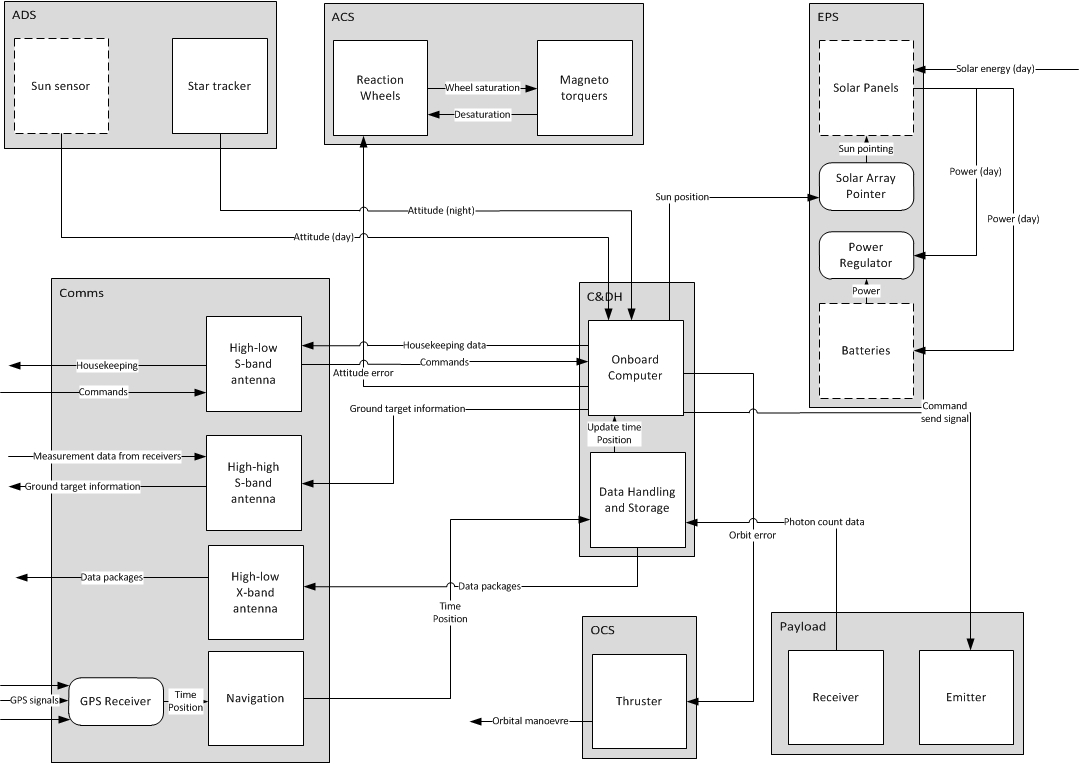
\includegraphics[width=1\textwidth, angle=90]{chapters/img/emitterHWblock.jpg}
\caption{Hardware block diagram emitter satellite}
\label{HWblockemitter}
\end{figure}

\begin{figure}
\centering
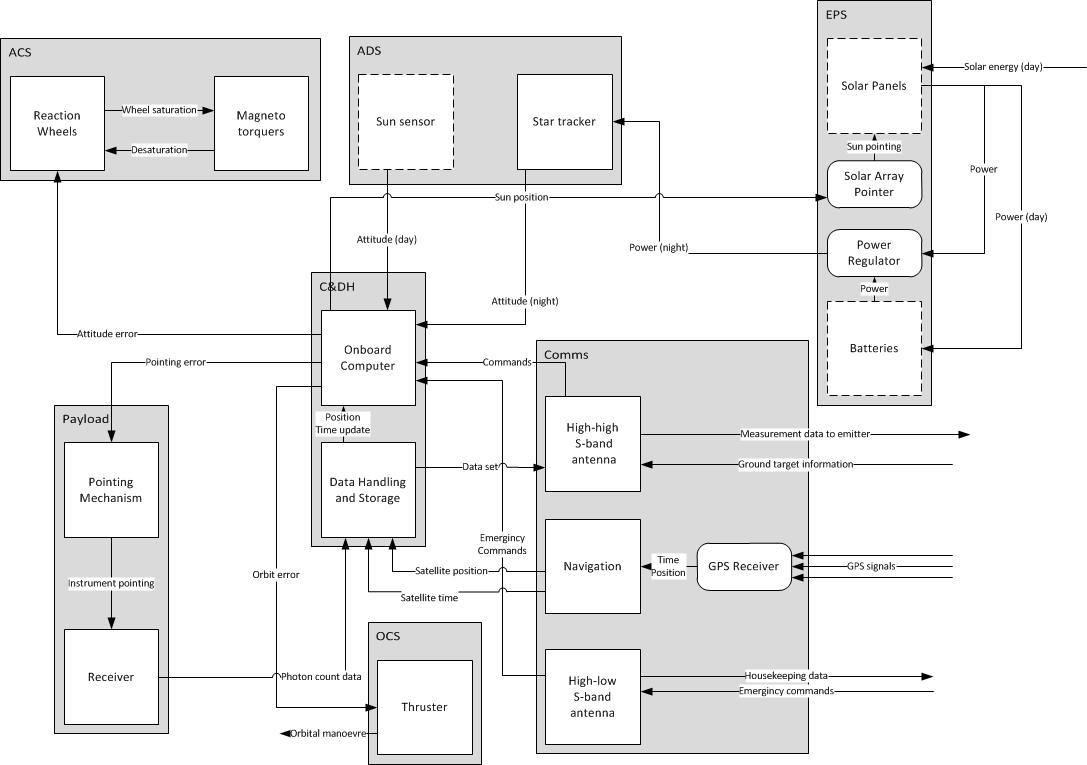
\includegraphics[width=1\textwidth, angle=90]{chapters/img/receiverHWblock.jpg}
\caption{Hardware block diagram receiver satellite}
\label{HWblockreceiver}
\end{figure}
\section{S/W Block Diagram}
\label{section_SWBD}

In the software block diagrams for the emitter satellite(Figure \ref{fig:SWBDemit} on page \pageref{fig:SWBDemit}) and the receiver satellite (Figure \ref{fig:SWBDrec} on page \pageref{fig:SWBDrec}) it can be seen how the different software modules interact with the output interfaces (represented by a circle) and the input interfaces (represented by a rhombus) of various devices on the satellite. 
 
Since the detailed implementation of the satellite software is outside of the scope of this project, the modules and interactions depicted are somewhat abstract.  

From the block diagram it can be seen that the Attitude \& Sun Position Processing Module is responsible for obtaining information from the \ac{ADS}, and pointing the satellite and solar panels in the appropriate direction. The Attitude \& Sun Position Processing Module works along with Receiver Pointing Determination Module to determine where to point the receiver. The Power Calculation Model determines whether to recharge or to use batteries based on the available solar power. Data storage is used to store all the data from various sensors for housekeeping purposes. The Photon-Location-Time Registration module registers position and time for Data Storage when a photon is received.

\begin{landscape}
\begin{figure}[ht!]
\centering
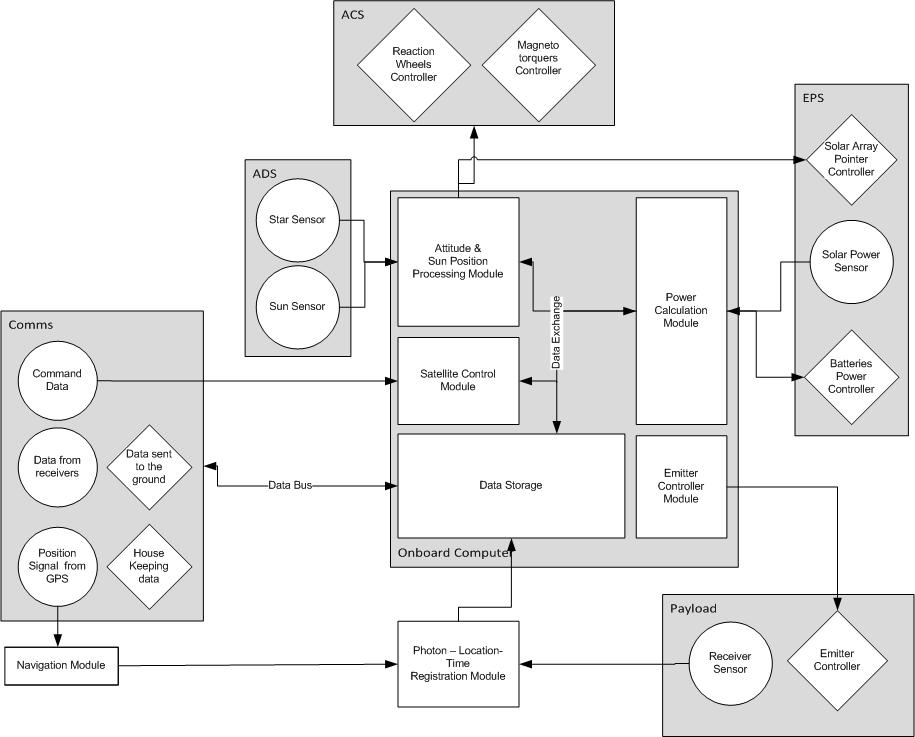
\includegraphics[width=1\textheight]{chapters/img/SWBDemit.jpg}
\caption{Software block diagram for emitter }
\label{fig:SWBDemit}
\end{figure}
\end{landscape}

\begin{landscape}
\begin{figure}[ht!]
\centering
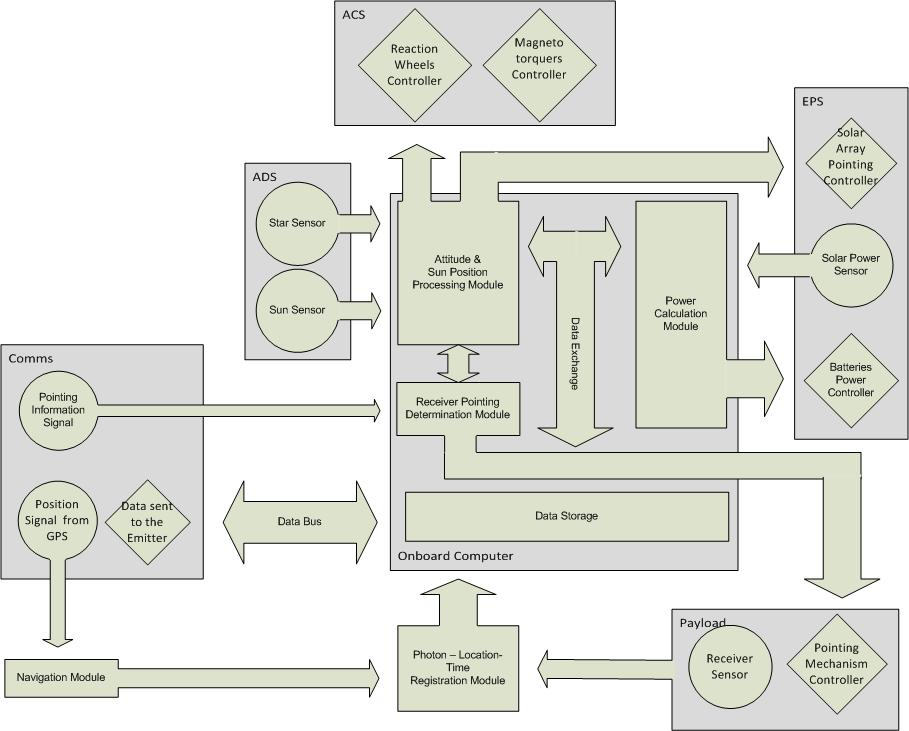
\includegraphics[width=1\textheight]{chapters/img/SWBDrec.jpg}
\caption{Software block diagram for receiver}
\label{fig:SWBDrec}
\end{figure}
\end{landscape}
\section{Electrical Block Diagram}
\label{EBD}

The electrical block diagrams show the architecture of the \ac{EPS} of the receiver and the emitter satellites. Detailed information about the block diagrams and the block diagrams themselves can be found in sections \ref{emitter_EPS} and \ref{receiver_EPS} for the emitter and receiver satellites respectively.

The electrical block diagram of the emitter satellite can be seen in figure \ref{fig:emitter_block} on page \pageref{fig:emitter_block} and that of the receiver satellites can be seen in figure \ref{fig:receiver_block} on page \pageref{fig:receiver_block}.
\section{Data Handling Block Diagram}
\label{DHBD}

This section is split into two parts, the first treats the data handling for the emitter satellite and the second for the receiver satellites.

\subsection{Data Handling for the Emitter}
\label{DataHandlingEmitter}

Figure \ref{fig:DHE}, on page \pageref{fig:DHE}, shows the data handling structure for the emitter satellite during nominal operating conditions. Nominal operating conditions refer to the state without any system failures. The rest of this section will contain some comments of the diagram is Figure \ref{fig:DHE}.

As can be seen the onboard computer is the most important part of the data handling subsystem. The term housekeeping data refers to all the data that indicate the spacecraft and its subsystems are in good health e.g. temperature, voltage, power, etc. It should also be noted that the S\&H arrow from the S-band antennae to the computer consists of science and housekeeping data from the receiver as well as housekeeping data of the emitter antennae. 

Furthermore the X-band phased array is only used to transmit science data, so the non-S arrows refer to the array itself. The S-band antenna mounted next to the X-band array handles data received from the ground, and housekeeping data sent towards the ground. The command arrow pointing to the S-band antenna are commands to the antenna itself, and the housekeeping is for the antenna only as well. Finally commands from the ground destined for the receiver satellites are directed from the computer to the S-band antennae aimed at the receiver satellites. So the command going to the S-band antennae block refers to commands for the antenna and for the receiver satellites.

\begin{figure}
\centering
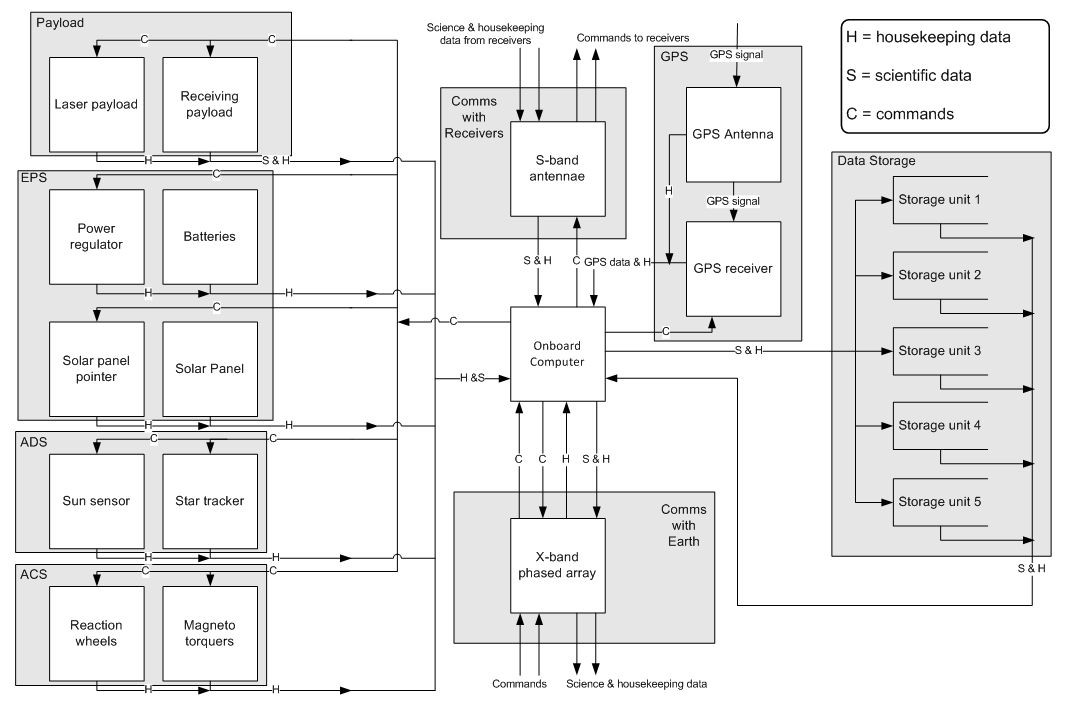
\includegraphics[width=1.0\textwidth, angle=90]{chapters/img/DHEmitter.png}
\caption{Figure showing the data handling structure for the emitter.}
\label{fig:DHE}
\end{figure}

\subsection{Data Handling for the Receiver}
\label{DataHandlingReceiver}

Figure \ref{fig:DHR}, on page \pageref{fig:DHR}, shows the data handling structure for any receiver satellite during nominal operating conditions. Nominal operating conditions refer to the state without any system failures. The rest of this section will contain some comments of the diagram is Figure \ref{fig:DHR}.

This diagram is very similar to the diagram for the emitter found on page \pageref{fig:DHE}. The main difference is the removal of the laser payload and of several storage units. The other main difference is the lack of an X-band array and S-band antenna for communications to the ground, instead only the S-band antennae for intersatellite communications remains. The command arrow going from the S-band antennae to the computer consists entirely of the commands send from the emitter, whereas the command arrow going toward the S-band antennae only contains commands meant for the antennae software. Also housekeeping data arrow from the S-band to the computer is data concerning only the antennae.

\begin{figure}
\centering
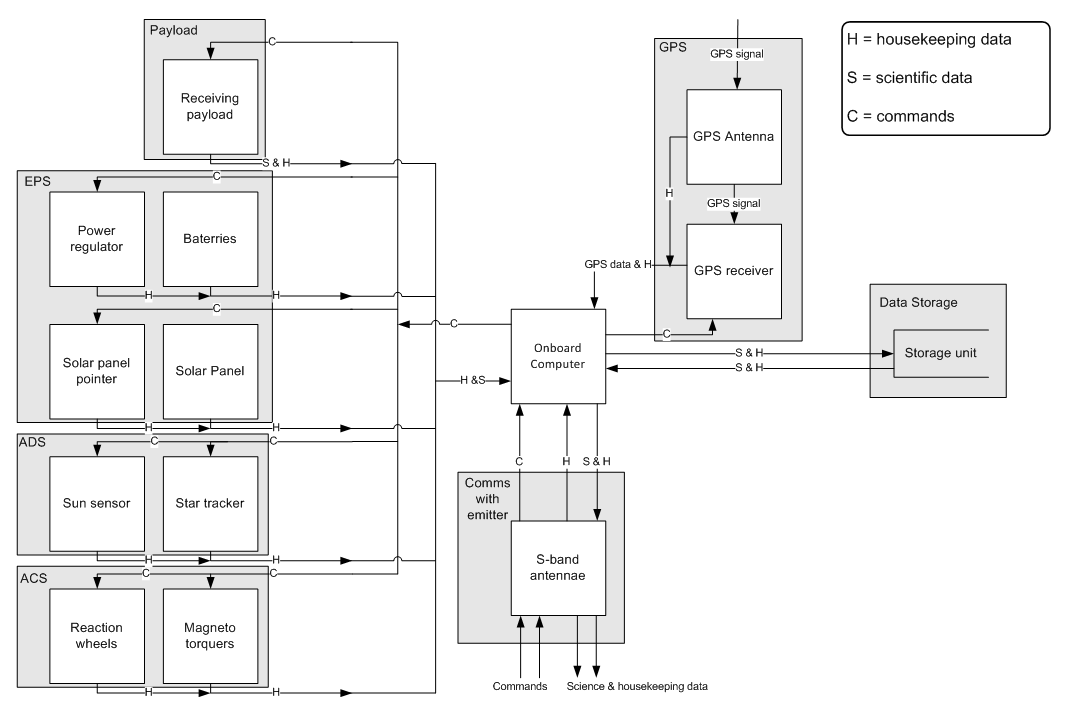
\includegraphics[width=1.0\textwidth, angle=90]{chapters/img/DHReceiver.png}
\caption{Figure showing the data handling structure for a receiver.}
\label{fig:DHR}
\end{figure}
\section{Communication Flow Diagram}

In this section the flow of communication within in the complete architecture (satellites and ground station) will be explained in detail.
\begin{figure}[ht]
\centering
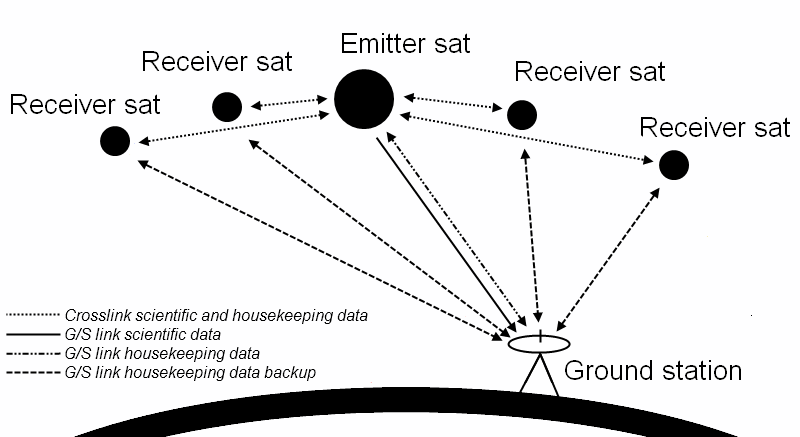
\includegraphics[width=1.0\textwidth, angle=0]{chapters/img/allesZW.png}
\caption{Complete communications architecture of the laser swarm}
\label{fig:allesZWW}
\end{figure}

Figure \ref{fig:allesZWW} on page \pageref{fig:allesZWW} shows all existing links and their place in architecture, with a legend in the lower left corner.
Three flows of communications exist in the architecture:
\begin{itemize}
\item Command data
\item Housekeeping data
\item Scientific data
\end{itemize}

Command data originates from the ground station, is transmitted to the emitter satellite over the G/S link for housekeeping and command data. In case the command data is required on a receiver satellite, the emitter satellite retransmits the data directly to that satellite over the crosslink for scientific, housekeeping and command data.

Housekeeping data flows in the exact reverse direction: the emitter satellite continuously receives the housekeeping data over the crosslinks from all the receiver satellites, then stores it and finally transmits it to the ground station together with its own housekeeping data over the G/S link for housekeeping data and command data.

In case the crosslinks are broken, command data and housekeeping data for and from the receiver satellites can still travel over the G/S link housekeeping and command data (backup).

The scientific data contains all the data on the registered photons (coordinates on the SPAD array, attitude and position of the satellites, timestamp). These are transmitted over the crosslinks to the emitter satellite, stored on its data storage system and then transmitted to the ground station over the G/S link for scientific data.

\section{Human Resource Allocation}
\label{DDHR}
The first part of the project will involve a team of five specialists designing the five critical subsystems and one person designing the orbits of the swarm. The other four members will concentrate on the development of the software that will be used to assist the trade-off and verify the design. At later stages, some of the the software engineering personnel is heavily involved in designing proper algorithms for the processing of mission data, while others will be brought in to assist with detail design. 

A schematic representation of the resource allocation can be found in figure \ref{fig:DDBBHR} on page \pageref{fig:DDBBHR}.

\begin{figure}[ht!]
\begin{center}
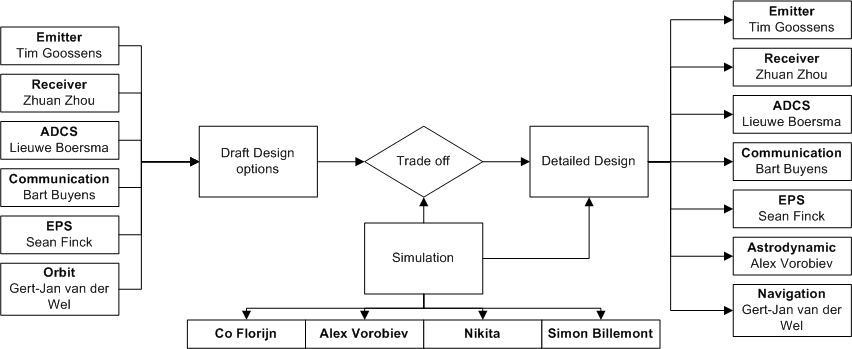
\includegraphics[width=0.9\textwidth]{chapters/img/DDBBHR.jpg}
\end{center}
\caption{Human resource allocation chart.}
\label{fig:DDBBHR}
\end{figure}

The table \ref{tab:RWD} on page \pageref{tab:RWD} gives the documentation distribution of each person on each chapter.
\begin{table}[ht!]
\centering
\scalebox{0.7}{
  
\begin{tabular}{|c|l|c|c|}
\hline
 Chapter & Documentation                      & Author & Checked by \\\hline 
 -       & Title Page                           & Alex   & \\\hline                  
 -       & Preface                              & Co, Team& \\\hline
 -       & List of Symbol                       &\\\hline
 -       & List of Acronyms                       &\\\hline
 -       & Abstract                             & Co, Bart &\\\hline
 1       & Introduction                         &\\\hline\hline
 2       & Project Management                   &\\\hline
 2.1     & \ -Resource Allocation               & Zhuan &\\\hline
 2.2     & \ -Budget Breakdown                  & Zhuan &\\\hline
 2.3     & \ -Operations and Logistic Concept Description&\\\hline
 2.4     & \ -Project Design and Development Logic & GJ &\\\hline
 2.5     & \ -Project Gantt Chart               & Lieuwe &\\\hline\hline
 3       & Mission Approach                     &\\\hline
 3.1     & \ -Function Flow Diagram             & Lieuwe, Zhuan & \\\hline
 3.2     & \ -Function Breakdown Structure      & Lieuwe, Zhuan &\\\hline
 3.3     & \ -H/W Block Diagram                 & Lieuwe, &\\\hline
 3.4     & \ -S/W Block Diagram                 &\\\hline
 3.5     & \ -Electrical Block Diagram          &\\\hline
 3.6     & \ -Data Handling Block Diagram       &\\\hline\hline
 4       & Risk Management                      & Tim, Zhuan & \\\hline\hline
 5       & Launch and Astrodynamic Characteristics & Alex &\\\hline
 5.1     & \ -Launch Segment                    & Alex &\\\hline
 5.2     & \ -Space Segment                     & Alex &\\\hline
 5.3     & \ -Space Environment and Shielding   & Alex &\\\hline\hline
 6       & Emitter                              &\\\hline
 6.1     & \ -OEP                               & Tim &\\\hline
 6.1.1   & \ \ -Principle of Diode Laser       & Tim &\\\hline
 6.1.2   & \ \ -Diode Pumped Laser Configuration & Tim &\\\hline
 6.1.3   & \ \ -Optical Characteristics        & Tim &\\\hline
 6.1.4   & \ \ -Diffraction                    & Tim &\\\hline  
 6.1.5   & \ \ -Thermal Control                & Tim, Lieuwe &\\\hline
 6.1.6   & \ \ -Laser Life Time Expectancy     & Tim &\\\hline
 6.1.7   & \ \ -Laser Focus Calculation        & Zhuan &\\\hline
 6.2     & \ -Navigation                        & GJ &\\\hline
 6.3     & \ -Communication                     & Bart &\\\hline
 6.4     & \ -ADCS                              & Lieuwe &\\\hline
 6.5     & \ -EPS                               & Sean &\\\hline
 6.6     & \ -Summary                           &\\\hline\hline
 7       & Receiver                             &\\\hline
 7.1     & \ -ORP                               & Zhuan &\\\hline
 7.1.2   & \ \ -SPAD Research                  & Tim, Zhuan &\\\hline
 7.1.3   & \ \ -Prism Design                   & Zhuan &\\\hline
 7.1.4   & \ \ -Summary                        & Zhuan &\\\hline
 7.1.5   & \ \ -Payload Cost Estimation        & Tim, Zhuan &\\\hline
 7.1.6   & \ -Navigation                        & GJ &\\\hline
 7.2     & \ -Communication                     & Bart &\\\hline
 7.3     & \ -ADCS                              & Lieuwe &\\\hline
 7.4     & \ -EPS                               & Sean &\\\hline
 7.5     & \ -Summary                           &\\\hline\hline
 8       & Data Validation                      & Simon, Co, Nikita &\\\hline
 8.1     & \ -Software Tool Internals           & Simon, Co, Nikita &\\\hline
 8.2     & \ -Validation Results                & Simon, Co, Nikita &\\\hline
 9       & Sustainable Development Strategy     &\\\hline
 10      & Compliance Matrix                    &\\\hline\hline
 11      & Conclusion & Recommendations         &\\\hline\hline
 -       & Others                               &\\\hline
 -       & \ -Catia Drawing                     & Lieuwe &\\\hline
 -       & \ -Latex Compile                     & Alex &\\\hline

\end{tabular}
}
\caption{Report writing distribution.}
\label{tab:RWD}
\end{table}

%%%%%%%%%%%%%%%%%%%%%%%%%%%%%%%%%%%%%%%%%%%%%%%%%%%%%%%%%%%%%%%%%%%%%%%%%%%%%%%%%%%%%%%%%%%%%
\section{Mass Budget Breakdown}
\label{DDMBB}
The table \ref{tab:MB} on page \pageref{tab:MB} indicates mass budget breakdown for emitter and receiver satellites. The table is mainly divided into two parts. The first part gives each subsystem mass of emitter and receiver satellites in both kilograms and percentage of total dry mass. Meanwhile, the second part includes the mass of propellants and then also gives the total mass when the satellites are in their orbit. The deviation of all numbers in the table can be found in each corresponding chapter of the subsystem.

\begin{table}[ht!]
\centering
\begin{tabular}{|l|c|c|c|c|}
\hline
 & \multicolumn{2}{|c|}{Emitter} & \multicolumn{2}{|c|}{Receiver} \\\hline
 Subsystem        & $M [kg]$ & \%$M_{dry}$ & $M [kg]$ & \%$M_{dry}$ \\\hline\hline
 Communication    & 10.66    & 21          & 3        & 22.2 \\\hline
 Navigation       & 0.25     & 0.5         & 0.25     & 1.85 \\\hline
 OEP              & 15       & 29.8        & -        & - \\\hline
 ORP              & 0.22     & 0.4         & 0.22     & 1.63 \\\hline
 EPS              & 5.8      & 11.5        & 3.6      & 26.6 \\\hline
 ADCS             & 2        & 4           & 2        & 14.8 \\\hline
 Thermal          & 1.48     & 3           & 0.3      & 2.22 \\\hline
 Structure        & 12.35    & 24.5        & 2.45     & 18.12 \\\hline
 Propulsion(tank) & 1        & 2           & 0.75     & 5.55 \\\hline
 Thruster         & 0.65     & 1.3         & 0.15     & 1.11 \\\hline
 Shielding        & 1        & 2           & 0.8      & 5.92 \\\hline\hline
 $M_{dry}$        & 50.41    & 100         & 13.52    & 100 \\\hline
 $M_{propellant}$ & 4        & -           & 1.5      & - \\\hline
 $M_{Loaded}$     & 54.41    & -           & 15.02    & - \\\hline
 $M_{Orbit}$      & 53.1     & -           & 14.92    & - \\\hline
\end{tabular}
\caption{Mass Budget Breakdown of the emitter and a representative receiver satellites.}
\label{tab:MB}
\end{table}

%%%%%%%%%%%%%%%%%%%%%%%%%%%%%%%%%%%%%%%%%%%%%%%%%%%%%%%%%%%%%%%%%%%%%%%%%%%%%%%%%%%%%%%%%%%%%
\section{Cost Budget Breakdown}
\label{DDCB}
Figure \ref{fig:lifecycle} on page \pageref{fig:lifecycle} shows a typical life-cycle for a space mission. The \ac{RDTE} stage includes the planning, development and testing of all prototypes and qualification units, but does not include the technology development for different subsystems. In the case of the laser swarm this is largely dependent on the single emitter and one receiver unit. This stage is also mostly consistent of non-recurring costs. The production stage consists of actual manufacture of the physical satellites. The cost estimation in this stage is based on the \ac{TFU}. This is done because it is assumed that the first unit (in the case of the Laser Swarm, that would be the emitter and one receiver) would be the most expensive to produce. The rest of the swarm constellation satellite costs are calculated by taking a theoretical learning curve \cite{larson}. 

\begin{figure}[ht!]
\centering
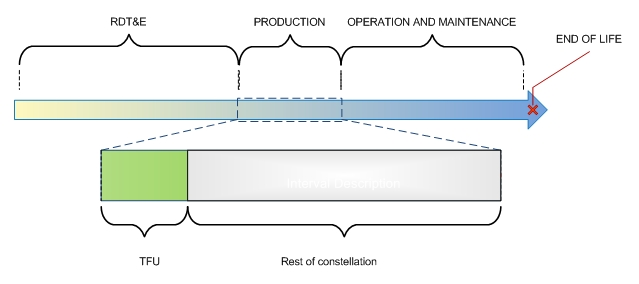
\includegraphics[scale = 0.8]{chapters/img/lifetime.jpg}
\caption{Satellite Life-Cycle}
\label{fig:lifecycle}
\end{figure}

The table \ref{tab:CB} on page \pageref{tab:CB} gives the cost breakdown of both theoretical first unit cost for either emitter or receiver satellite and also the swarm of 9 satellites including all the wraps.

\begin{table}[ht!]
\centering
\begin{tabular}{l|c|c|c|c|c|c|}
\cline{2-7}
  & \multicolumn{4}{|c|}{Unit Cost} & \multicolumn{2}{|c|}{\multirow{2}{*}{Swarm (9 satellites)}} \\\cline{2-5}
  
  & \multicolumn{2}{|c|}{Emitter satellite} & \multicolumn{2}{|c|}{receiver satellite} & \multicolumn{2}{|c|}{ } \\\hline
  
 \multicolumn{1}{|c|}{Subsystem} & Cost [k\$] & \%Subtotal & Cost [k\$] & \%Subtotal & Cost [k\$] & \%Subtotal \\\hline
                                     %  cost [k$] %Total 
 \multicolumn{1}{|l|}{Payload}       & 8215.96 & 41.5 & 4048.74 & 46.58 & 8660 & 25.3 \\\hline
 \multicolumn{7}{|l|}{Bus Total}     \\\hline
 \multicolumn{1}{|l|}{Structure}     & 1920.38 & 9.7 & 843.2 & 9.7 & 3322.33 & 9.7 \\\hline
 \multicolumn{1}{|l|}{Thermal}       & 217.776 & 1.1 & 95.62 & 1.1 & 376.76 & 1.1 \\\hline
 \multicolumn{1}{|l|}{EPS}           & 541 & 2.7 & 266 & 3.06 & 1193.694 & 3.49 \\\hline
 \multicolumn{1}{|l|}{Navigation}    & 25   & 0.13 & 25 & 0.29 & 191.235 & 0.558 \\\hline
 \multicolumn{1}{|l|}{Communication} & 2940 & 14.9 & 612.5 & 7.05 & 7141.14 & 20.85 \\\hline
 \multicolumn{1}{|l|}{\acs{ADCS}}    & 199.093 & 1 & 175.914 & 2.02 & 1405.687 & 4.1 \\\hline
 \multicolumn{1}{|l|}{Tank}          & 0.713 & 0.0036 & 0.428 & 0.0049 & 3.649 & 0.011 \\\hline
 \multicolumn{1}{|l|}{Thruster}      & 570.64  & 2.88 & 356.65  & 4.1 & 3016.9 & 8.8 \\\hline
 \multicolumn{7}{|l|}{Wraps}     \\\hline
 \multicolumn{1}{|l|}{\acs{IAT}}     & 1445.24 & 7.3 & 634.58 & 7.3 & 2500.34 & 7.3 \\\hline
 \multicolumn{1}{|l|}{Program Level} & 2395.53 & 12.1 & 1051.84 & 12.1 & 4144.36 & 12.1 \\\hline
 \multicolumn{1}{|l|}{\acs{GSE}}     & 692.92 & 3.5 & 304.25 & 3.5 & 1198.78 & 3.5 \\\hline
 \multicolumn{1}{|l|}{\acs{LOOS}}    & 633.53 & 3.2 & 278.17 & 3.2 & 1096.03 & 3.2 \\\hline
 \multicolumn{1}{|l|}{Subtotal}      & 19797.79 & 100 & 8692.92 & 100 & 34250.88 & 100 \\\hline
 \multicolumn{1}{|l|}{Launch}        & - & - & - & - & 18534.25 & - \\\hline\hline\hline
 \multicolumn{1}{|l|}{Total}         & - & - & - & - & 52785.13 & - \\\hline
 \multicolumn{1}{|l|}{Total (FY00)}  & - & - & - & - & 43089.90 & - \\\hline
 
\end{tabular}
\caption{Cost Budget Breakdown.}
\label{tab:CB}
\end{table}

%%%%%%%%%%%%%
%
%       RISK MANAGEMENT
%
%%%%%%%%%%%%%

\chapter{Risk Management}
\label{chap:risk_management}
\input{chapters/DDrisk.tex}

%%%%%%%%%%%%%
%
%       Astrodynamics
%
%%%%%%%%%%%%%
\chapter{Launch and Astrodynamic Characteristics}
\label{chap:astrodynamics}
This chapter explains the characteristics of the launch and space segments of the mission. Section \ref{frLS} describes the three main parts in bringing the swarm into the orbit: launch vehicle, launch location and orbit insertion. Section \ref{frSS} discusses all the aspects of the constellation and its configuration, and delves into estimations of $\Delta$V and needed propellant. Finally, section \ref{frSEaS} deals with the hazardous space environment and ways of protecting the satellites against it. 

\section{Launch Segment}
\label{frLS}

The launch segment of the mission includes the selection of the launch vehicle, the launch location and the procedure of inserting the satellites into their respective orbits. The following subsections discuss all of these aspects. 

\subsection{Launch Vehicle}
\label{frLSLV}

The costs of launch vary greatly between different vehicles. Table \ref{table:vehicleCosts} on page \pageref{table:vehicleCosts} lists approximate total launch costs of respective platforms. For consistency, the prices are given in Fiscal Year 2000 dollars.
\begin{table}[h]
\begin{centering}
\begin{tabular}{llr}
\toprule
Platform & Operator & Price (FY00M\$) \\
\hline \hline
Ariane V  & ESA & 97.96 \\
Soyuz   & Starsem or Arianespace&  8.16 - 22.1 \\
Vega   & European and Italian SA  & 15.1 \\
Falcon 1E  & SPACEX  & 8.89 \\
PSLV & ISRO & 13.88 - 16.33 \\
Rokot & Eurokot & 9.8 - 11.4 \\
\bottomrule
\end{tabular}
\caption{Estimated price comparison of different launch vehicles. \emph{(Source: various.)}}
\label{table:vehicleCosts}
\end{centering}
\end{table}

Based on the information  in the above table it is possible to single out a few platforms which will be affordable for the purpose of this feasibility study. The values represent the total launch segment costs. The Ariane V launcher is the most expensive option by far and would push the budget quite heavily, with an estimated cost of launch almost half of the total budget. However the payload capabilities of the Ariane V launcher far outweigh that of all other platforms, thus making it possible for a combined launch with other satellites, leading to shared costs. This however could jeopardize the mission in the sense that it becomes secondary priority. If that happens, the constellation would have higher requirements for orbit acquisition: an extra booster stage or higher onboard fuel capacity for the altitude and/or plane shift, which is not feasible. The Ariane V is therefore an unsuitable platform for this project. 

The rest of the launchers can be analyzed with respect to reliability. All of the launch vehicles have been tested, with the exception of the Vega system, which is yet to make its maiden flight. The Vega is therefore not suitable for the analysis at this time. It is for this reason that the project will no longer consider this system at all.  However, better data should be available in the near future which should allow for the Vega platform to be reevaluated.

The same goes for the Falcon 1e. The launcher is an incremental improvement on the Falcon 1, of which only the last two launches out of five were successful. This technology is not proven enough for the purpose of the mission.

Table \ref{table:LVreliability} on page \pageref{table:LVreliability} shows some reliability statistics for the remaining 3 vehicles.

\begin{table}[h]
\begin{centering}
\begin{tabular}{lcccp{5cm}}
\toprule
Platform & Total No. of Launches & Total Failures & Reliability & No. of Successful Launches Since Last Failure  \\
\hline \hline
Soyuz   & 1754  &  88 & 95\% & 57 \\
PSLV & 16 & 1 & 94\% & 15 \\
Rokot & 17& 2 & 88\% & 6 \\
\bottomrule
\end{tabular}
\caption{Reliability figures for several launch vehicles. \emph{(Source: various.)} }
\label{table:LVreliability}
\end{centering}
\end{table}

The Soyuz launch vehicle presents itself as the most reliable platform, with a track record that far surpassed all other options. This launch vehicle will be the one considered for this project. In the next section, its payload capabilities are discussed.

\subsubsection{Soyuz LV Payload Capability Analysis}
\label{frLVPCA}

There is a large selection of Soyuz vehicles available for consideration. For the purpose of this project, the newest modification - Soyuz-ST will be used. This vehicle is part of the Soyuz-2 family, which are technologically superior to the older Soyuz-U and U2 launchers. An illustration and technical parameters of the Soyuz-ST can be found in Appendix \ref{appa} on page \pageref{appa} \cite{soyuzman}.

An estimation of mass performance for the launch vehicle can be seen in figure \ref{fig:massperformance} on page \pageref{fig:massperformance}.

\begin{figure}[ht]
\centering
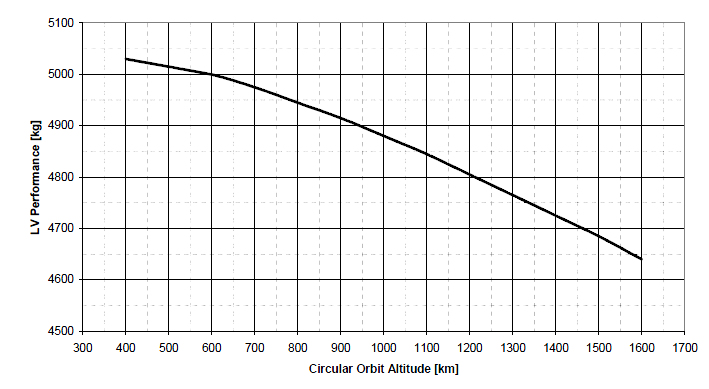
\includegraphics[width=0.6\textwidth, angle=0]{chapters/img/lvmass.png}
\caption{Mass performance of the Soyuz-ST for circular orbits. \emph{(Source: \cite{soyuzman}.})}
\label{fig:massperformance}
\end{figure}

The payload mass data provided in \cite{soyuzman} is estimated, yet is good enough to have a reasonable idea about the maximum mass. The Soyuz-ST is able to launch roughly a maximum of 5000 kg into a 500 km orbit. This is well above the design mass of the formation thus will allow for further considerations of joint launches (as long as the swarm mission is considered to be the primary payload) and thus spread launch costs. 

The available volume in the Soyuz-ST Fairing can be seen in figure \ref{fig:soyuzvol} on page \pageref{fig:soyuzvol}.

\begin{figure}[ht!]
\centering
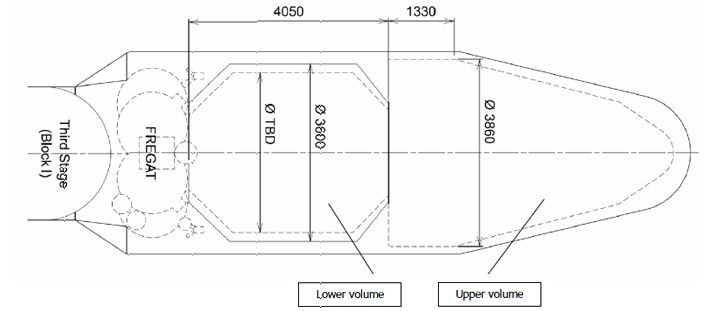
\includegraphics[width = 0.8\textwidth, angle=0]{chapters/img/soyuzvolRotated.png}
\caption{Fairing volume of the Soyuz-ST launch vehicle. Here shown in dual launch carrying configuration.\emph{ Source: \cite{soyuzman}.}}
\label{fig:soyuzvol}
\end{figure} 

The dimensions of the fairing are visibly too large and there is no possibility of using a different one, however that leaves a lot of possibilities for different designs of release adapters to adapt to the unique sequence of separation upon orbit injection. Again, the possibility of taking other small satellites along on the same launch arises. The dual launch configuration shown in the previous figure is the one being considered for the launch.

The choice of the Soyuz brings forth one more advantage: the use of a unique orbit insertion booster, the Fregat. This final stage will allow for minimization of fuel on the satellite as all orbit insertion maneuvers can be done using the Fregat. The Fregat stage has been designed to handle 20 individual burns.

\subsubsection{Vibrational Analysis}
\label{frLVCA}
The launch is a critical part of the mission for the survival of the payload. It is during this period that the payload will experience the most severe loads. In this section the origin and magnitude of these loads will be discussed, as well as their impact on the payload. The main loads are the quasi-static loads, shock loads, sinusoidal loads, random vibrations and acoustic vibrations.

Quasi-static loads are caused by the engine thrust. The acceleration will increase steadily as the amount of fuel becomes less. Peaks are reached when the engines run out of fuel and stop giving thrust. The ignition of a stage also results in a peak load. These loads are all in the longitudinal direction. There are also quasi-static loads in the lateral direction caused by ground maneuvers and wind gusts. These kind of loads are expressed as load factors. The maximum load factors for the Soyuz launcher are $+1,5/-5\ g$ in longitudinal direction and $+1,8/-1,8\ g$ in lateral direction.

Shock loads are high acceleration loads over a short period of time. They are mostly the result of separation events such as the separation of the boosters, different stages of the launcher and the payload fairing. They also occur with the deployment of appendages such as the solar panels. The shock response spectrum of some launchers is given in figure \ref{fig:SRS} on page \pageref{fig:SRS}.

\begin{figure}[ht!]
\centering
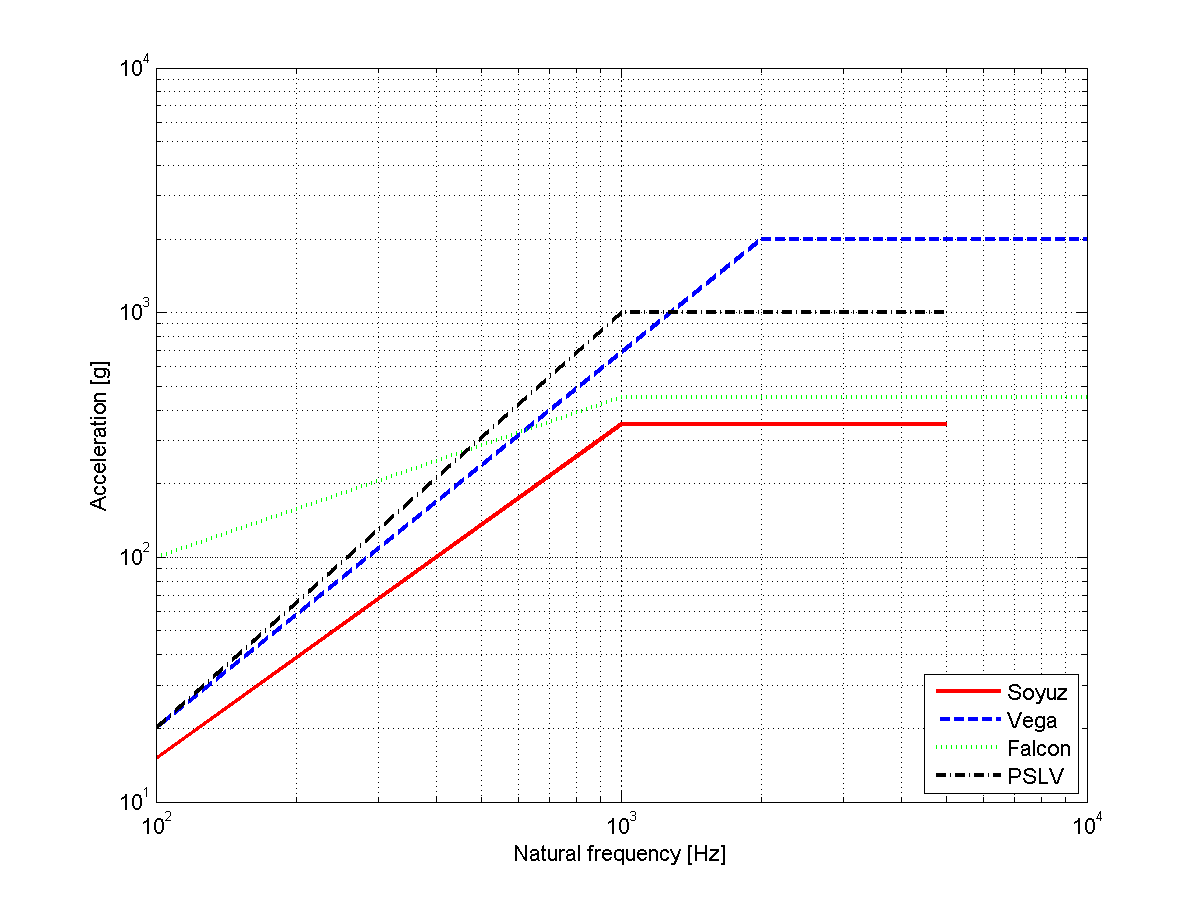
\includegraphics[width=0.5\textwidth, angle=0]{chapters/img/Shock_Loads_Acceleration.png}
\caption{Launch shock response spectrum as a function of payload natural frequency.}
\label{fig:SRS}
\end{figure}

The release of the payload from the adapter also causes a shock load, but with smaller accelerations than during launch. Ruag space has developed a low-shock release mechanism (\ac{CBOD}). The \acs{CBOD}'s shock response spectrum is shown in figure \ref{fig:CBOD_SRS} on page \pageref{fig:CBOD_SRS}.

\begin{figure}[ht!]
\centering
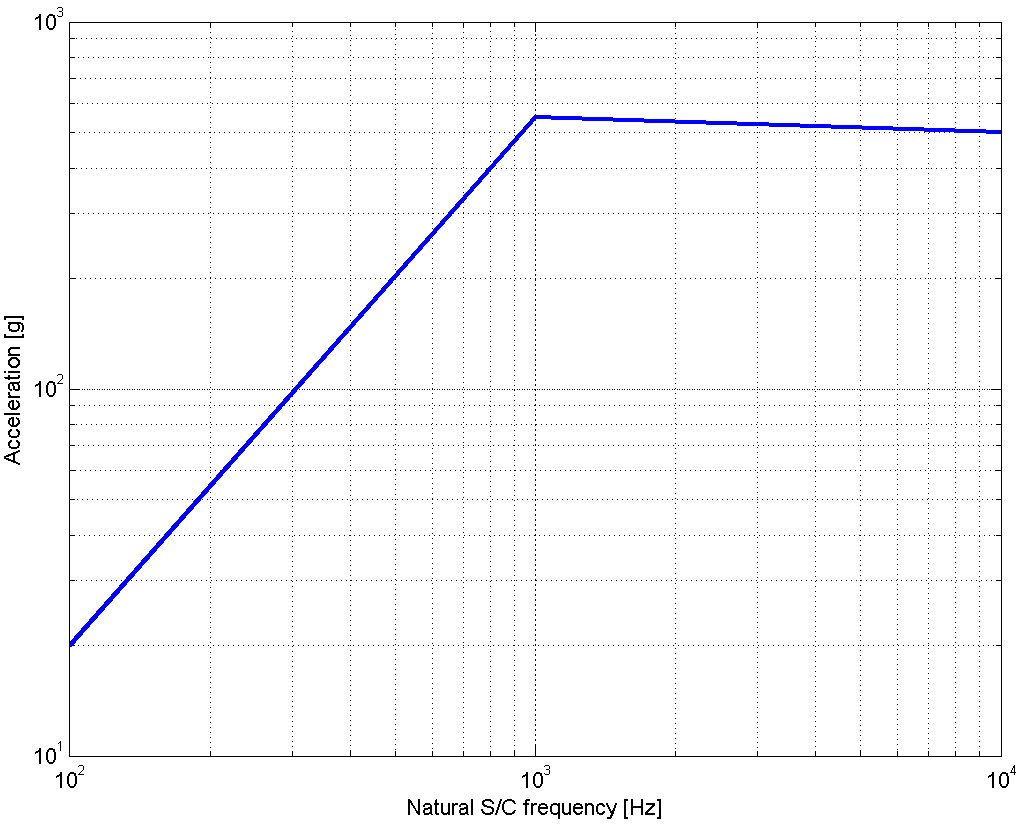
\includegraphics[width=0.5\textwidth, angle=0]{chapters/img/CBOD_release_acceleration.png}
\caption{Shock response spectrum of the \acs{CBOD} release mechanism.}
\label{fig:CBOD_SRS}
\end{figure}

Another critical load source are random vibrations. For the Soyuz launcher, only random vibrations between 20 and 100 Hz need to be taken in to account because higher frequencies are covered by acoustic vibrations. Random vibrations are caused by the propulsion system and the vibro-acoustic response of the neighboring structures. Table \ref{tab:random_vibr} on page \pageref{tab:random_vibr} gives the power spectral density, root mean square vibration and the duration of the sources for each part of the launch.

\begin{table}[H!]
\centering
\begin{tabular}{ccccc}
\toprule
 Event & \multicolumn{2}{c}{PSD $[g^2/Hz]$} & $G_{rms} [g]$ & Duration [s] \\
 \midrule
 Frequency band [Hz] & 20 - 50 & 50 - 100 & & \\
 \midrule
 First stage flight & 0.005 & 0.005 - 0.01 & 4.94 & 120 \\
 Second stage flight & 0.0025 & 0.0025 & 3.31 & 480 \\
 Third stage flight & 0.0025 & 0.005 & 3.31 & 480 \\
 Fregat flight & 0.002 & 0.002 & 1.63 & 875 \\
 \bottomrule
 \end{tabular}
 \caption{Soyuz maximum random vibrations \emph{ Source: \cite{soyuzman}.}}
\label{tab:random_vibr}
\end{table}

Acoustic vibrations are higher than random vibrations, up to 10 000 Hz. The main sources are the acoustic noise that radiates from the engines and from aerodynamic turbulence when the launcher passes through the trans-sonic part of the flight. During ground operations the venting system also produces noise. For the Soyuz launcher, this does not exceed 94 dB. Apart from the lift-off and the trans-sonic part of the flight, the acoustic vibrations are rather low. The structures that are affected the most by acoustic loads are structures with a low mass and high surface area, such as solar panels and skins sections. Table \ref{tab:acoustic_vibr} gives the acoustic noise spectrum under the fairing.

\begin{table}[H!]
\centering
\begin{tabular}{cc}
\toprule
Octave Center & Flight limit level [dB]\\
Frequency [Hz] & (reference: 0 dB = 2 X $10^{-5} Pa$ ) \\
\midrule
31.5 & 125\\
63 & 132 \\
125 & 134 \\
250 & 136 \\
500 & 134 \\
1000 & 125 \\
2000 & 121 \\
\bottomrule
 \end{tabular}
 \caption{Soyuz acoustic noise spectrum \emph{ Source: \cite{soyuzman}.}}
\label{tab:acoustic_vibr}
\end{table}

Sinusoidal loads occur mainly during the atmospheric flight. They are caused by lift off, bending of the rocket motors, aerodynamic buffeting and oscillations in the propulsion system. To avoid these kind of vibrations, the payload must be constructed in such a way that the payload's natural frequencies will not be close to those of the launcher. This will avoid resonance and thus the payload will experience much lower loads. For the Soyuz launcher it is required that the natural frequencies of the payload will be higher than 15 Hz in lateral direction and higher than 35 Hz in longitudinal direction. 

\subsection{Launch Site}
\label{frLSLS}

The selection of the launch site relies on several factors:

\begin{itemize}
	\item Availability of attainable inclinations from launch.
	\item Compatibility with the launch vehicle.
	\item Accessibility and cost.
	\item Security and political reasons. 
\end{itemize}

The first factor is crucial. It is paramount that the satellites are injected into their final inclinations at launch and do not have to perform any inclination change maneuvers, which require a substantial amount of $\Delta$V. With this in mind choosing a launch site closer to the equator is necessary. Launch sites at higher latitudes would need to sacrifice velocity and thus payload mass because of their location. Table \ref{table:launchtable} on page \pageref{table:launchtable} shows a number of possible launch sites and their locations \cite{larson}. The list contains only the sites compatible with the Soyuz-ST launch vehicle. Furthermore, in figure \ref{fig:launchsites} on page \pageref{fig:launchsites}, the same sites are indicated with their respective authorized inclination ranges.

\begin{table}[ht!]
\begin{centering}
\begin{tabular}{llp{2cm}p{2cm}}
\toprule
Launch Site & Operator & Latitude (deg min) & Longitude (deg min) \\
\hline \hline
Baikonur LC-31/6  & Russia (Starsem) & 45 54 N & 63 18 E \\
Plesetsk LC-43  & Russia (Starsem)   &  62 48 N & 40 24 E \\
Guiana Space Centre  ELS  & CNES/Arianespace  & 5 18 N & 52 50 W \\
\bottomrule
\end{tabular}
\caption{Available launch sites for the Soyuz-ST. \emph{(Source: \cite{larson}.)}}
\label{table:launchtable}
\end{centering}
\end{table}  

\begin{figure}[ht!]
\centering
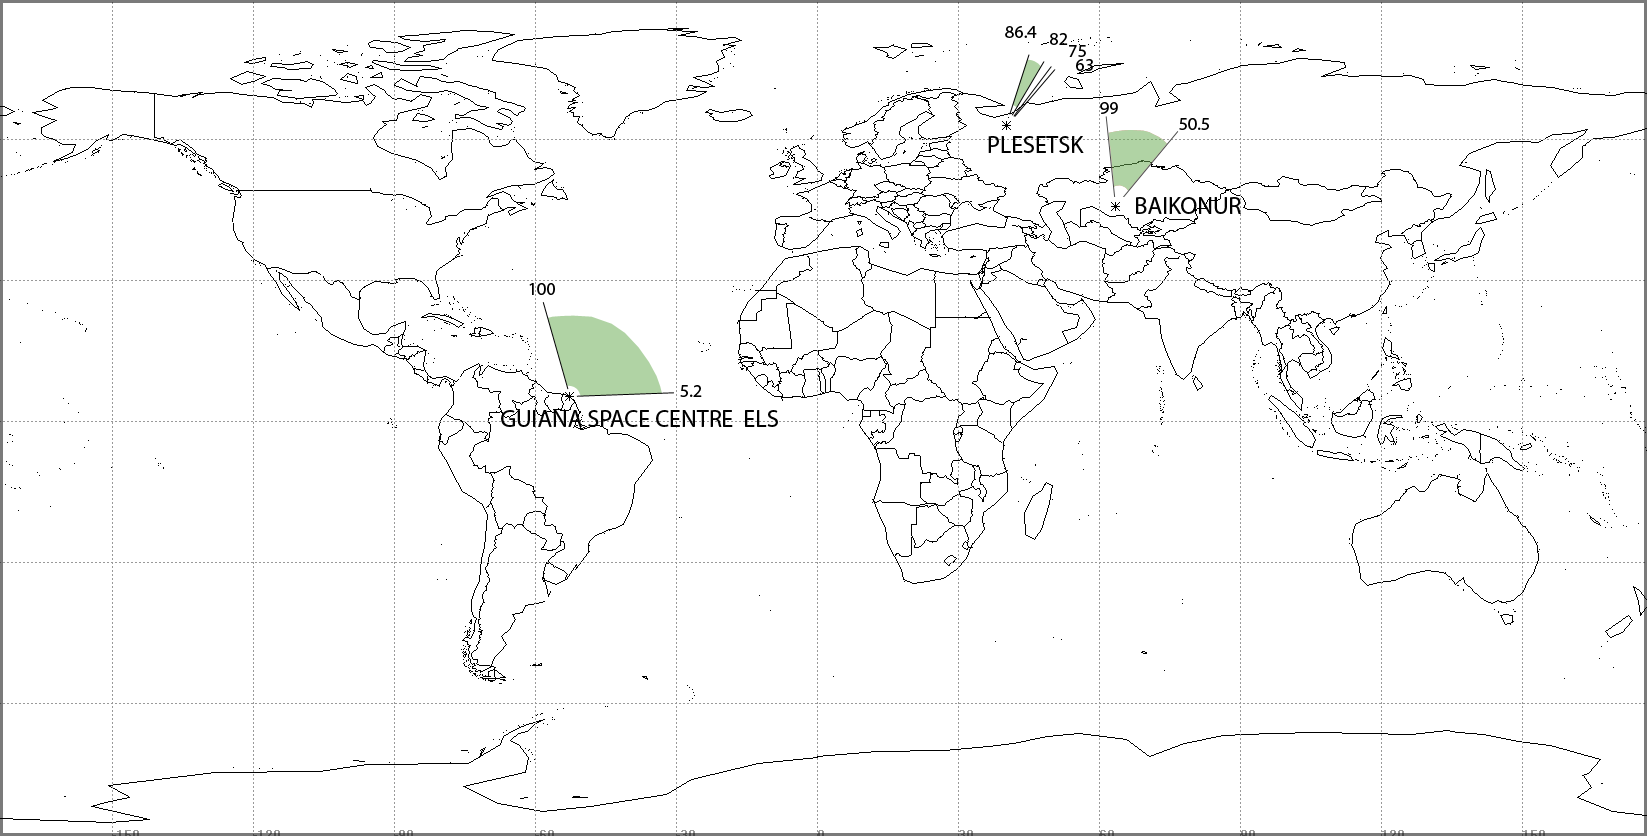
\includegraphics[width=1.0\textwidth, angle=0]{chapters/img/launchsites.png}
\caption{Launch site locations and allowable inclinations for the Soyuz-ST. \emph{(Sources: \cite{constDesign} and \cite{rockotman}.)} }
\label{fig:launchsites}
\end{figure}

Even though all the sites in table \ref{table:launchtable} allow inclinations of 85 degrees, it is still preferable to select a site closer to the equator in order to utilize the full effect of Earth's rotation and lower the launch costs. With this in mind, the Guyana Space Centre is selected to be the preferable location for launch.

The \ac{ELS} in Kourou, Guyana is currently being finalized and should accommodate its first Soyuz launch in 2010 \cite{arianesoyuz}.

A typical launch profile of the Soyuz launch vehicle from Kourou is shown in figure \ref{fig:launch} on page \pageref{fig:launch}. The first three stages of the vehicle are used to propel the payload and the Fregat booster in to a circular orbit at around 200 km. After separation (stage 6 on the figure), the Fregat initiates the first orbit injection burn to bring the satellites to the appropriate orbits.

\begin{figure}[ht]
\centering
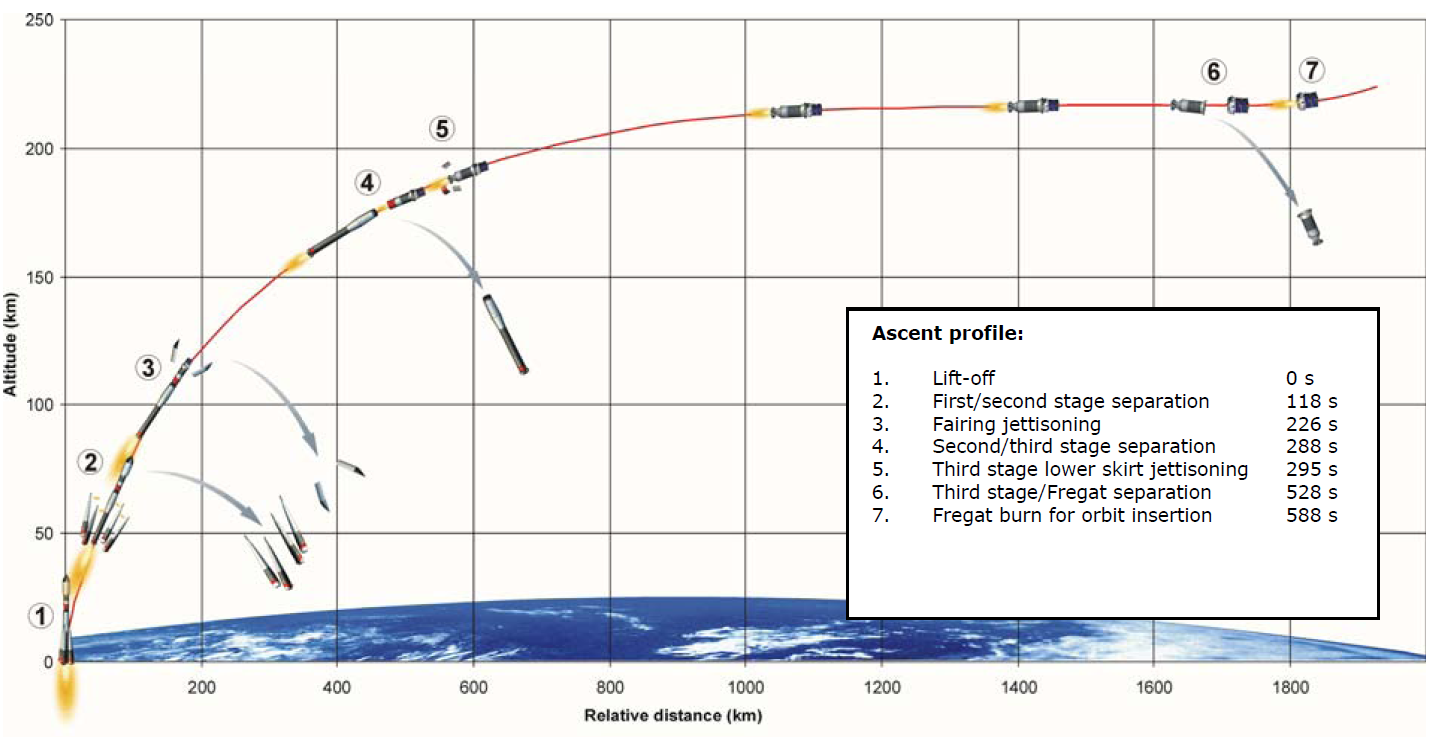
\includegraphics[width=1.0\textwidth, angle=0]{chapters/img/launchprofile.png}
\caption{Launch profile of the Soyuz LV from Kourou. \emph{(Sources: \cite{soyuzman}.)} }
\label{fig:launch}
\end{figure}

With this information it is possible to further calculate some important launch parameters:

\begin{itemize}
	\item The inertial velocity of the launch site is given by:
	
	\begin{equation} 
 		V_L = (464.5) cos L 
	\end{equation}
	
	where $L$ is the site latitude. For the case of Kourou the inertial velocity is 462.51 m/s.
	\item The launch azimuth in the inertial frame of reference is given by:
	
	\begin{equation} 
 		A_{Z_I} = arcsin(\frac{cos i}{cos L})
	\end{equation}
	
	and is equal to 5.022 degrees for this launch.
	\item The launch azimuth corrected for the Earth's rotation, is given by:
	
	\begin{equation} 
 		A_Z = arctan(\frac{V_0sinA_{Z_I}-V_{eq}cosL}{V_0cosA_{Z_I}})
	\end{equation}
	
	where $V_0$ is the orbital velocity reached by the launcher before separation and the first burn of the Fregat upper stage (see above, around 7.784 km/s), $V_{eq}$ is the velocity of the Earth's rotation at the equator - 464.5 m/s. Thus the corrected launch azimuth becomes 1.61 degrees. 
	
	\item The required launch velocity is calculated to be 7.76 km/s which means that due to Earth's rotation 26.8 m/s are saved.
\end{itemize}

Furthermore the region is politically stable and the launch site is under the protection from the French government and other security forces. All safety procedures are kept to the highest of standards and the spaceport is easily accessible by air or sea (Source: \cite{soyuzman}).

\subsection{Orbit Insertion}
\label{frLSOI}

The orbit insertion is separated into two distinct stages: primary orbits and secondary orbits. The primary orbits are located at an altitude of 500 km and contain the emitter and four initial receivers. The secondary orbits are located at a slightly different altitude of 525 km and contain the auxiliary receivers intended for replenishment.

The configuration of the primary orbits is discussed in section \ref{frSSSC} and an image of the formation can be seen in figure \ref{fig:confmax} on page \pageref{fig:confmax}. The release sequence and the important parameters are as follows (for satellite and orbit numbers please refer to figure \ref{fig:confmax}):

\begin{enumerate}
	\item The Fregat is injected in Orbit 1.
	\item The ascending intersection of Orbit 1 and Orbit 2 is reached at a latitude of 85$^{\circ}$ and a longitude offset (from the ascending node of Orbit 1) of 88.91$^{\circ}$. At this point the Fregat should be orientated in the direction of Orbit 2 and separate Rec 2. The separation $\Delta$V that the adapter should produce is calculated using:
	
	\begin{equation} 
 		\Delta V = 2 V_i sin \frac{\alpha}{2}
	\end{equation}
	
	where $V_i$ is the orbital velocity (7.612 km/s) and $\alpha$ is the relative inclination (2.17$^{\circ}$, see section \ref{frSSSC}) \cite{spacedesign}. The $\Delta$V is calculated to be 289.63 m/s.
	
	\item As the Fregat crosses the descending node and approaches the second plane intersection of the orbit, it does not need to change orientation (Orbit 3 intersects in the same direction on the descent phase as Orbit 2 does on the ascent phase). At the intersection Rec 1 is separated with a $\Delta$V of 289.63 m/s. This is a very large value thus the method of deployment should be thoroughly investigated in a further design. 
	\item After this the Fregat again aligns with the velocity vector of Orbit 1.
	\item The Frigate should inject itself into a drift orbit with a negative drift rate of no less then 9.19 deg/orbit and re-injected back to Orbit 1 after traveling $90+\Delta \phi /2 = 90.09505$ degrees. This will bring the launcher 2.3 degrees behind the final emitter position, or 0.12 degrees behind Rec 4.
	\item At this point the remaining three satellites: Rec 3, Base and Rec 4 should be put into drift orbits by the attachment mechanism in order to acquire the 2.18 degree orbital separation. The exact order and timing can be designed and adjusted accordingly.
\end{enumerate}

After this, the satellites can be considered to be in their orbits. The Fregat can start the burn to insert into the secondary orbits. Once the altitude of 525 km is reached the Fregat performs a plane shift to change its \ac{RAAN} to approximately 10 degrees behind that of the primary orbit. The exact angle has to be carefully acquired through careful modeling of differential node precessions as the satellites decay. The general idea is that the secondary satellites should have the correct \acp{RAAN} by the time they decay to arrive in the right position with respect to the emitter.  The formation in the secondary orbit is the same as in the primary orbits minus the emitter, thus similar maneuvers have to be performed.

\subsection{Launch Date}
\label{frLSLD}

The launch date is dominated by development times and lifetime considerations. The satellite orbit decay and thus the lifetime is a function of the atmospheric density. The density is, in turn, a function of the solar activity. The number of sun spots on the surface of the sun rises and falls every eleven years. The measurements are commonly represented in 10.7 cm radio flux intensities. Figure \ref{fig:f10.7} on page \pageref{fig:f10.7} presents a projection for the next 10 years.

\begin{figure}[h]
\centering
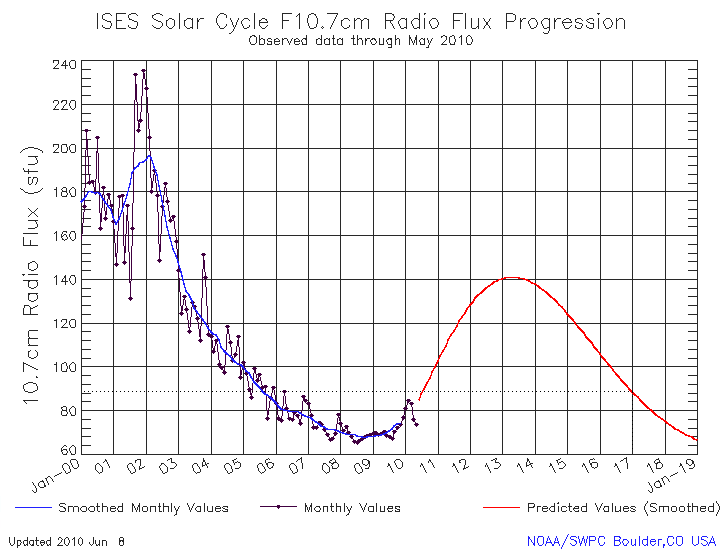
\includegraphics[width=0.6\textwidth, angle=0]{chapters/img/solarCycle.png}
\caption{Solar activity projection up to 2019. \emph{(Source: NOAA/Space Weather Prediction Center.)} }
\label{fig:f10.7}
\end{figure}

In order to provide the longest possible lifetime for the mission it is essential that the launch is timed in such a way that the satellites are in orbit most of the time during solar minimum. For this reason a launch on March 1st 2017 is planned. This also gives enough time for development and production. For further information on the timeline, please refer to section \ref{frPMgantt}.

\section{Space Segment}
\label{frSS}

This section covers the astrodynamical characteristics of the mission. The emitter orbit is covered first, then in section \ref{frSSRO}, all receiver orbits are examined. The formation and its properties are discussed in section \ref{frSSSC}. Collision avoidance is described in section \ref{frSSCA} and, finally, section \ref{frSEaS} covers the orbital environment and whether the mission is going to be heavily affected by it. 

\subsection{Emitter Orbit}
\label{frSSEOD}

\subsubsection{Orbital Parameters}
\label{frSSEODOP}

The emitter satellite is injected into a circular orbit at an altitude of 500 km. The eccentricity is frozen at 0. Inclination is chosen to be 85 degrees, as this allows access to polar areas, which are places of interest for the mission. Furthermore, the inclination provides an inherent relative phase for the crossing orbits. The \acl{RAAN} can be chosen arbitrary for the start of the mission, as no specific target is assumed for the mission. For consistency, in all following discussions it is assumed to be 0 degrees. The same goes for the Argument of Perigee and the True Anomaly. As the orbit is circular, these values are not really relevant. The emitter satellite acts as the reference for all the receiver satellites.

The orbit is non-sunsynchronous and does not have a specific repeat track. This allows for larger coverage of the Earth. 

Figure \ref{fig:confmax} on page \pageref{fig:confmax} shows the emitter satellite (labeled as Base) in Orbit 1.

A few basic properties of this orbit can be derived and are shown in table \ref{table:orb1ref} on page \pageref{table:orb1ref}. All the values were generated with the help of \cite{larson}, \cite{spacedesign} and \cite{constDesign}.

\begin{table}[!h]
\begin{centering}
\begin{tabular}{lccr}
\toprule
Parameter				&			Symbol			&			Value			&			Unit \\
\hline \hline
Altitude				&			h						&			500				&			[km]	 \\
Semi-major Axis	&			a						&			6871			&			[km]	 \\
Eccentricity		&			e						&			0				  &			[-]	 \\
\acs{RAAN}			&			$\Omega$		&			0				&			[deg]	 \\
Period (mins)		&			P						&			94.6135	&			[mins]	 \\
Revolutions per day		&									&			15.2198	&			[revs/day]	 \\
Angular Velocity		&			n						&			3.805	&			[deg/min]	 \\
Circular Velocity		&			V						&			7.6127	&			[km/s]	 \\
Max. Eclipse		&			 	$T_e$					&			35.75	&			[mins]	 \\
Node Spacing	&			 						&			23.72	&			[deg]	 \\
Node Precession	&			 $\dot{\Omega}$					&			-0.6667	&			[deg/day]	 \\
\bottomrule
\end{tabular}
\caption{Orbital properties of the emitter satellite.}
\label{table:orb1ref}
\end{centering}
\end{table}
%--------------
\subsubsection{Orbit Decay}
\label{frEmOD}
Atmospheric drag is by far the most relevant perturbation for \ac{LEO} satellites that causes loss of altitude and thus decays the orbit. It directly relates to mass as it influences the amount of fuel required to maintain the orbit, where as the mass influences the rate at which the orbit decays. Altitude selection relies heavily on estimation and analysis of drag data as for longer mission times, higher altitudes are preferred, while optical instruments prefer lower altitudes for increased accuracy.

The drag that the satellite experiences due to atmospheric density is described by the following formula:

\begin{equation}
D = -\frac{1}{2} C_D \rho V^2A
\label{drag}
\end{equation}

It follows that orbital parameter changes (semi-major axis, period and velocity respectively) per orbit are calculated using the following equations (assuming negligible eccentricity):

\begin{equation}
\Delta a = -2 \pi \left( C_D \frac{A}{m} \right) \rho a^2
\label{deltaSMA}
\end{equation}
\begin{equation}
\Delta P = -6 \pi^2 \left( C_D \frac{A}{m} \right) \rho \frac{a^2}{V}
\label{deltaP}
\end{equation}
\begin{equation}
\Delta V = \pi \left( C_D \frac{A}{m} \right) \rho aV
\label{deltaV}
\end{equation}

The fundamental problem with accurately predicting effects due to atmospheric drag is twofold: firstly it is very hard to predict the satellite's ballistic coefficient:

\begin{equation}
\frac{m}{AC_D}
\label{ball}
\end{equation}

Even with a well known mass to area ratio, the coefficient of drag can be highly variable, highly dependent on the shape of the satellite and its orientation with respect to the velocity vector. It is usually determined in laboratory conditions. For the orbit decay analysis the following equation for the coefficient of drag was used:

\begin{equation}
C_D = \alpha C_{DS} + \beta C_{DD}
\label{cd}
\end{equation}

where $C_{DS}$ is the specular coefficient of drag, $C_{DD}$ is the diffuse coefficient of drag, $\alpha$ and $\beta$ are component fractions which are determined experimentally. The specular coefficient of drag is usually predominant. In reality this drag coefficient changes. The cross-sectional area normal to the velocity vector can also vary for the swarm satellites if the whole platform is reoriented for instrument pointing. These parameters were adjusted in such a way that a final average $C_D$ of 2.22 for the emitter as well as the receiver was achieved. This is a value which is commonly used in space mission design.

The cross-sectional area of the satellite perpendicular to the velocity vector for a sample period of 6 hours can be seen in figure \ref{fig:area} on page \pageref{fig:area}. The graph was generated using the correct geometry of the satellite simulated in the Satellite Tool Kit\texttrademark software, issued by AGI, Inc. The software also computes the mean area - 1.045948 m$^2$. This will be the area used for lifetime analysis. The mass used is the final estimated satellite loaded orbit mass from section \ref{DDMBB}. It is computed to be 22.87 kg/m$^2$. This is well within the normal range for regular satellites \cite{larson}.

\begin{figure}[ht!]
\centering
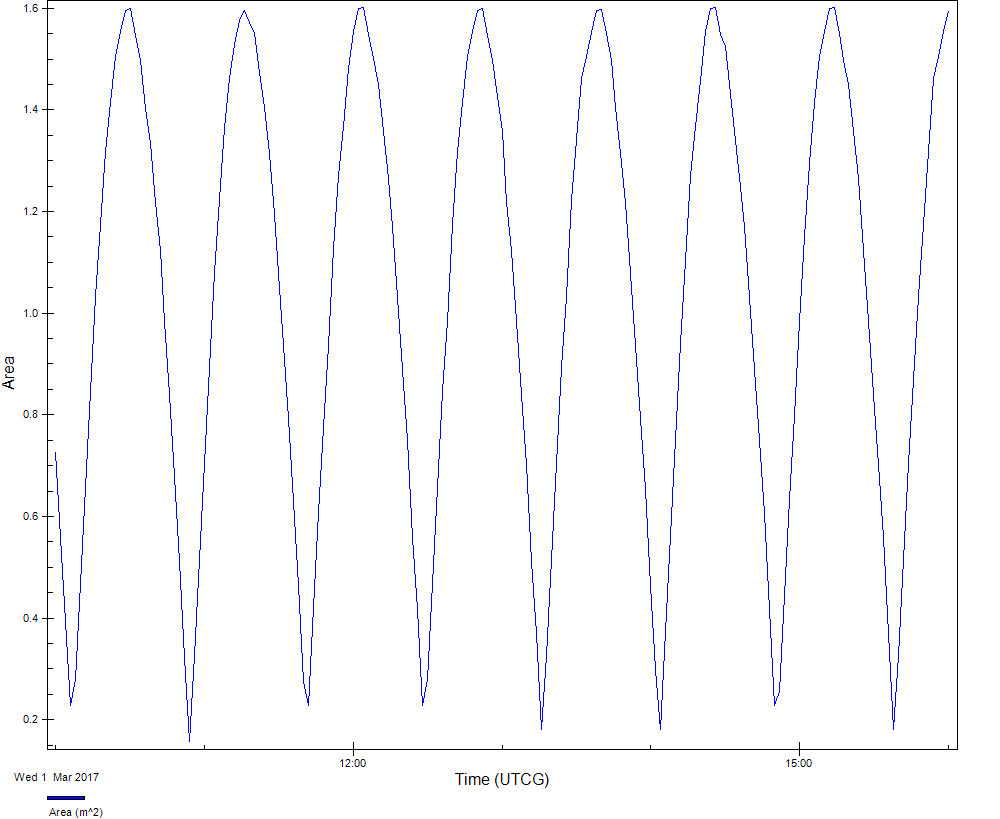
\includegraphics[width=0.4\textwidth, angle=0]{chapters/img/wetareaEmitter.png}
\caption{Simulated cross-sectional surface area of the emitter satellite perpendicular to velocity vector.}
\label{fig:area}
\end{figure}

The second reason drag calculations are so unreliable, is because air density at any altitude is highly variable. Raising air density is primarily connected with solar activity. As solar activity increases every 11 years the atmosphere heats up. Seemingly contrary to conventional gas laws that would dictate a fall in density as the gas expands, the atmosphere simply rises, increasing density at higher altitudes. This was previously discussed in section \ref{frLSLD}.

The density difference during solar maxima and minima for different altitudes is shown in figure \ref{fig:densityProfile} on page \pageref{fig:densityProfile}. Depending on the altitude, the density could vary for up to a whole order of magnitude between the minimum and maximum.

\begin{figure}[ht]
\centering
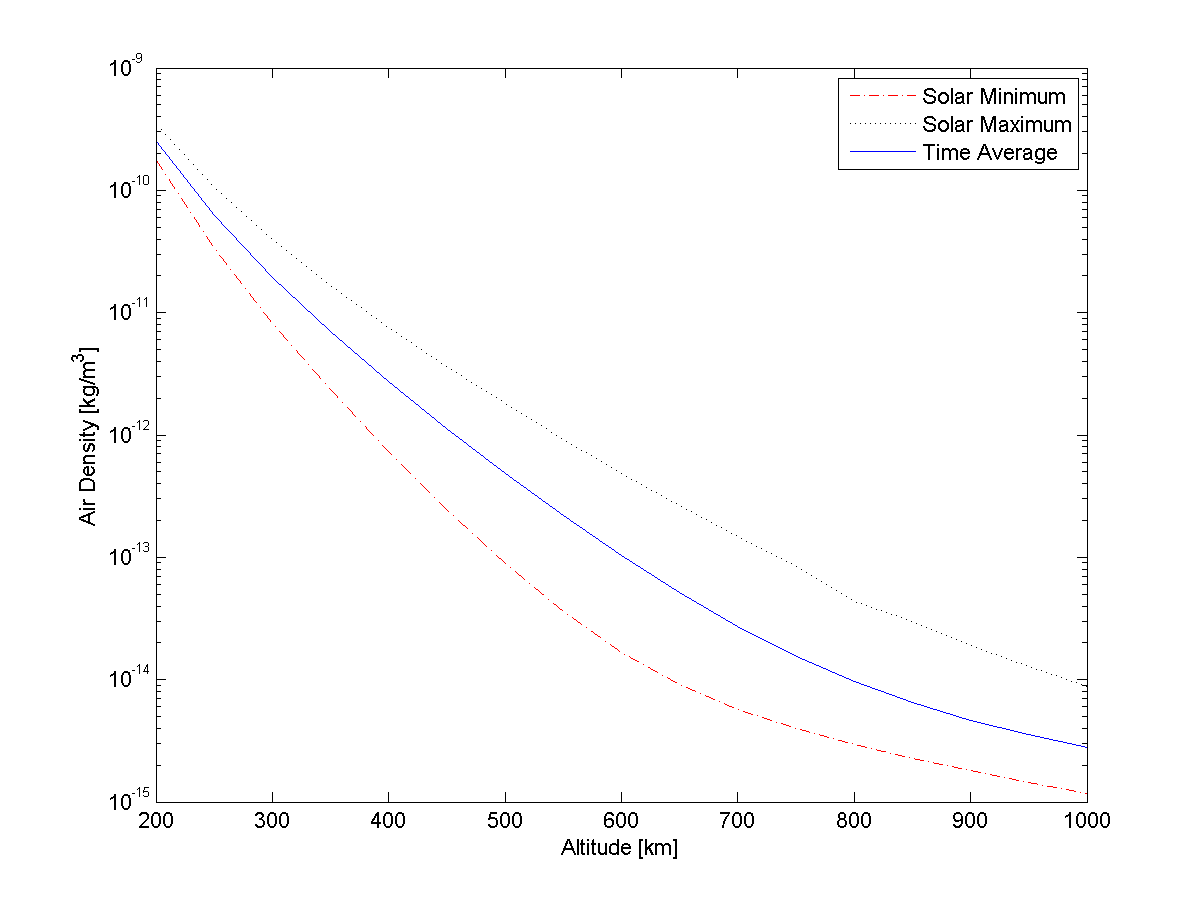
\includegraphics[width=0.5\textwidth, angle=0]{chapters/img/densityAltitude.png}
\caption{Air density vs. orbit altitude for different solar cycle stages.}
\label{fig:densityProfile}
\end{figure}

The orbit lifetime simulation was produced using the software package Satellite Tool Kit\texttrademark and can be seen in figure \ref{fig:emLife} on page \pageref{fig:emLife}.

The simulation performs orbit propagation up to the $J_4$ factor and uses the MSIS-86 Thermospheric Model for atmospheric density calculation. In addition it takes into account solar radiation pressure with an average sun exposed area of 0.84 (this area is also estimated from the satellite model simulations).

It is obvious from the previous figure that, unmaintained, the orbit would totally decay in 4.8 years. Another notable time is the point at which the emitter passes the 450 km altitude. This occurs at approximately 3.4 years after mission start. This is the altitude that will be considered as the absolute floor and will be used to approximate the altitude of the secondary satellite orbits.

\subsubsection{Estimation of $\Delta V$}
\label{frEmDV}

In order to properly estimate the mass of the propellant required for the mission all maneuvers have to be taken into account. Every maneuver requires a certain velocity change in a specified direction. During its mission, the emitter satellite will perform the following maneuvers:

\begin{itemize}
	\item A phase change slowdown. As the satellite was released from the booster vehicle, it was injected into a drift orbit in order to separate into a certain phase shift. Once this phase shift is achieved, the satellite needs to perform a boost to bring itself back into the circular orbit. This $\Delta V$ is equal and opposite to the $\Delta V$ induced by the release mechanism. This $\Delta V$ is calculated using the following equation:
	
		\begin{equation} 
 			\omega _{drift} = (1080)\frac{\Delta V}{V} 
		\end{equation}
	where $\omega _{drift}$ is the drift rate given in deg/orbit. For the emitter to return out of its drift orbit in 90 degrees, this maneuver requires a $\Delta V$ of 64.8 m/s.
	\item A boost to change the altitude from 450 km to 500 km after approximately 3.4 years in orbit. This maneuver is performed using a simple Hohmann transfer orbit and will require two burns. A simple transfer calculation is completed using the following method \cite{spacedesign}:
	\begin{equation} 
 			V_{450} = \sqrt{\frac{GM}{a_{450}}} =  7.6405\ km/s
		\end{equation}
		\begin{equation} 
 			V_{500} = \sqrt{\frac{GM}{a_{500}}} = 7.6127\ km/s
		\end{equation}
		\begin{equation}
			a_{ellipse} = \frac{a_{500}+a_{450}}{2} = 6853\ km
		\end{equation}
		\begin{equation} 
 			V_{p} = \sqrt{\frac{2GM}{a_{450}}-\frac{GM}{a_{ellipse}}} = 7.6544\ km/s
		\end{equation}
		\begin{equation} 
 			V_{a} = \sqrt{\frac{2GM}{a_{500}}-\frac{GM}{a_{ellipse}}} = 7.5988\ km/s
		\end{equation}
			\begin{equation}
			\Delta V_1 = 1000(V_p - V_{450}) = 13.9237\ m/s
		\end{equation}
		\begin{equation}
			\Delta V_2 = 1000(V_{500} - V_a) = 13.8984\ m/s
		\end{equation}
		\begin{equation}
			\Delta V = \Delta V_1 + \Delta V_2 = 27.8221\ m/s
		\end{equation}
		
		Thus the required $\Delta V$ for the Hohmann transfer is 27.8 m/s.
	\item A deorbit burn to take the satellite down to comply with sustainability requirements. This $\Delta V$ is approximated by the following equation \cite{constDesign}:
	
	\begin{equation}
			\Delta V_{deorbit} \approx V \left[ \frac{0.5(H_i - H_e)}{2R_E + H_i + H_e} \right]
		\end{equation}
	where $H_i$ is the initial altitude, $H_e$ is the reentry altitude and $R_e$ is the Earth's radius. Using the initial altitude of 500 km and a reentry altitude of 50 km, the $\Delta V$ is calculated to be 128.73 m/s. This is a very large value and in reality can be scaled down by considering a lower initial altitude (500 km is asumed in this analysis due to the consideration that a satellite might become disfunctional at the beginning at the mission and would need to be brought down) and a higher final reentry altitude (which is arbitrary). 
	
	\item The final consideration is the orbit injection accuracy of the Soyuz launch vehicle. The manufacturer states an inclination accuracy of 0.033 degrees for a 1000 km altitude orbit \cite{soyuzman}. For the purposes of this analysis, an accuracy of 0.03 degrees is used. The following equation is used to estimate the $\Delta V$ needed to correct this error:
	\begin{equation}
			\Delta V_{plane change} = 2V_i sin \frac{\alpha}{2}
		\end{equation}
	  where $V_i$ is the initial orbital velocity. The final $\Delta V$ is 3.99 m/s.
\end{itemize}

No $\Delta V$ is required for stationkeeping as the emitter will be allowed to decay naturally while the receivers will have to perform relative stationkeeping. Furthermore, the Soyuz launch vehicle can have a initial delivery altitude error. This is not considered, since it is assumed that as long as the constellation is delivered to the same altitude, no correction will be required and the lifetime of the mission will not be jeopardized. 

The total $\Delta V$ required for the emitter is calculated to be approximately 225.38 m/s.



%-------------

\subsection{Receiver Orbits}
\label{frSSRO}

\subsubsection{Orbital Parameters}
\label{frSSRODOP}

Unlike the emitter, the receiver satellites are placed in six different orbits and have to be designed to be able to handle all orbits and yet all the satellites have to have the same mass configuration at all times.

The orbits are divided into primary and secondary. The primary orbits are shown in figure \ref{fig:confmax} on page \pageref{fig:confmax}. Receiver 1 is located in Orbit 3 which has all the same orbital characteristics of Orbit 1 as described in section \ref{frSSEODOP} with the exception of its \acs{RAAN} having a value of +2.18 degrees. This is the maximum angle of separation and is derived from the requirement of a laser reflection angle of 30 degrees. Receiver 2 in Orbit 2 on the other hand has a \acs{RAAN} of -2.18 degrees. Both of these receiver satellites pass their ascending nodes at the same time as the emitter satellite. The reason for this is that the inclination of the orbits induces a relative phase between the satellites which is favorable for collision avoidance.

Receivers 3 and 4 are placed on the same orbit as the emitter. Receiver 3 travels with a positive phase offset of 2.18 degrees in front of the emitter, while the latter is trailing the emitter with the same offset. All orbital velocities and other parameters are identical to those described in section \ref{frSSEODOP}.

The secondary orbits are designated 1S, 2S and 3S, and are arranged in a similar manner while having an orbital altitude of 525 km. Receivers 1S, 2S, 3S and 4S also correspond in their arrangement to their primary counterparts.

Parameters of the secondary orbits that are different to those of the primary are shown in table \ref{table:orbsecref} on page \pageref{table:orbsecref}.

\begin{table}[ht!]
\begin{centering}
\begin{tabular}{lccr}
\toprule
Parameter				&			Symbol			&			Value			&			Unit \\
\hline \hline
Altitude				&			h						&			525			&			[km]	 \\
Semi-major Axis	&			a						&			6896			&			[km]	 \\
Period (mins)		&			P						&			95.1298	&			[mins]	 \\
Revolutions per day		&									&			15.1372	&			[revs/day]	 \\
Angular Velocity		&			n						&			3.7843	&			[deg/min]	 \\
Circular Velocity		&			V						&			7.6127	&			[km/s]	 \\
Node Spacing	&			 						&			23.85	&			[deg]	 \\
Node Precession	&			 $\dot{\Omega}$					&			-0.6584	&			[deg/day]	 \\
\bottomrule
\end{tabular}
\caption{Orbital properties of the secondary orbits (only the parameters different to those of the primary orbits are shown).}
\label{table:orbsecref}
\end{centering}
\end{table}

The initial RAANs are yet to be determined and a very complex model is required to account for differential precessions between the primary and secondary orbits. This is crucial in order for the secondary constellation to arrive in the right place with respect to the emitter. The calculations though fall out of the scope of this investigation.

\subsubsection{Orbit Decay}
\label{frRecOD}

The orbit decay analysis is done in a manner identical to that described in section \ref{frEmOD}. The final loaded mass of all the primary receiver satellites should be the same as the final orbits are established in order to decay at the same rate. The mean drag area estimated with the STK\texttrademark software is 0.3 m$^2$. The loaded mass is taken from section \ref{DDMBB}. The area exposed to the sun (for solar pressure) is calculated to be 0.25 m$^2$. The ballistic coefficient then becomes 22.40 kg/m$^2$, which is extremely close to that calculated for the emitter satellite, certainly within the margins at this point in the design. This is key to maintaining the constellation. The final design of all the satellites should ensure they decay in the closest possible manner.

The results of the decay simulation can be seen in figure \ref{fig:recLife} on page \pageref{fig:recLife}. They are virtually the same as the decay shown in figure \ref{fig:emLife}.

The decay rate of secondary satellites is shown in figure \ref{fig:recLife2} on page \pageref{fig:recLife2}. The actual altitude was iterated in order to see that the receivers would decay to 500 km in mid August 2020. In reality the secondary satellite will have to take 0.3 kg of fuel less then the primary (at the expense of less fuel available for the deorbit maneuver) as the emitter satellite would have lost 27.8 m/s worth of propellant after the Hohmann transfer back to 500 km. This will ensure the same decay rate of the secondary leg of the mission.    


\subsubsection{Estimation of $\Delta V$}
\label{frRecDV}

During the mission different receiver satellites will require different $\Delta V$. The main concern is to equalize them as the final orbits are established. The differences are only different due to different phase shifts needed and different orbital velocities.

The satellites will need to perform the following maneuvers:

\begin{itemize}
	\item A phase shift maneuver similar to the one described in section \ref{frEmDV}. For this maneuver different drift rates are required for the satellites. Receivers 1 and 2 will need a $\Delta V$ of 32.42 m/s (drift rate assumed to be half an orbit). Receiver 3 would require 31.58 m/s, but would require an entire orbit to establish its position. Receiver 4 would require a mere 0.85 m/s.
	
	The secondary orbit satellites have a different circular velocity thus also have different $\Delta V$'s. Receivers 1S and 2S require 32.37 m/s. Receiver 3S needs 31.52 m/s, and finally, Receiver 4S requires 0.84 m/s.
	\item The deorbit maneuver will require the same $\Delta V$ for all primary satellites and is also equivalent to the that of the emitter - 128.73 m/s. The secondary satellites will require 27.8 m/s less (100.93 m/s in total) as explained earlier.
	\item The correction for orbit insertion is identical for all primary satellites - 3.99 m/s (see section \ref{frEmDV}). Secondary satellites need a $\Delta V$ of 3.98 m/s. This difference is neglegible.  
\end{itemize}

The total $\Delta V$ for each receiver satellite is computed in table \ref{table:dVrec} on page \pageref{table:dVrec}.

\begin{table}[!h]
\begin{centering}
\begin{tabular}{lcccccc}
\toprule
				&			R1/R2			&			R3			&			R4		& R1S/R2S & R3S & R4S \\
\hline \hline
Phase shift				&			32.42						&			31.58		&			0.85		& 32.37 & 31.52 & 0.84	 \\
Deorbit				&			128.73						&			128.73		&			128.73		& 100.93 & 100.93 & 100.93	 \\
Inclination Correction			&			3.99						&			3.99		&			3.99		& 3.98 & 3.98 & 3.98	 \\ \hline \hline
\textbf{Total	}		&			165.14						&			164.3		&			133.57		& 137.28 & 136.43 & 105.75	 \\
\bottomrule
\end{tabular}
\caption{Total $\Delta V$ for individual receiver satellites. Values are given in m/s.}
\label{table:dVrec}
\end{centering}
\end{table}

The largest $\Delta V$ (i.e 165.14 m/s) was used for propulsion system design.

Again no numbers are specified for stationkeeping. This topic is elaborated on in section \ref{frSSStation}.

%------------------
\begin{figure}[ht!]
\centering
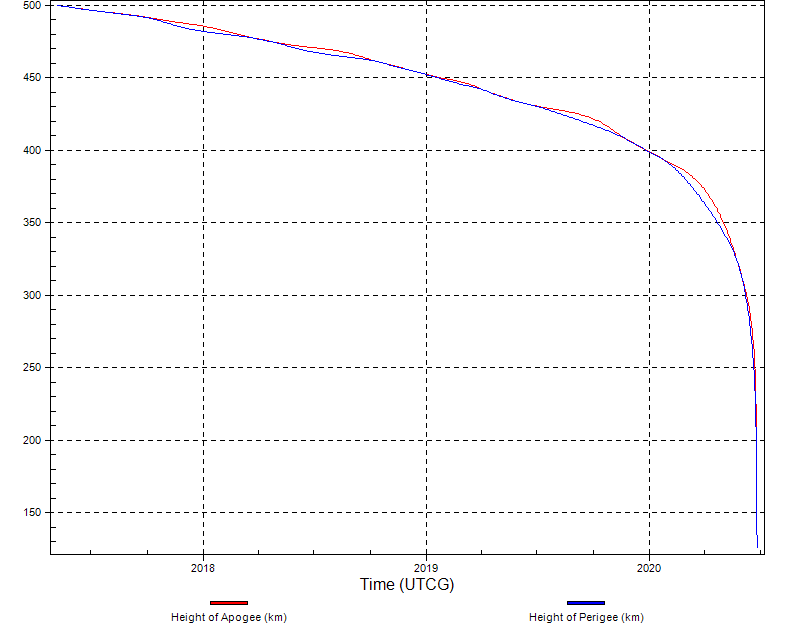
\includegraphics[width = 0.75\textwidth]{chapters/img/emitterDecay.png}
\caption{Emitter satellite orbit decay with an assumed mission start in March 2017. Values used: $C_D = 2.22$, $mass = 53.1 kg$, $area = 1.046 m^2$.}
\label{fig:emLife}
\end{figure}

\begin{figure}[ht!]
\centering
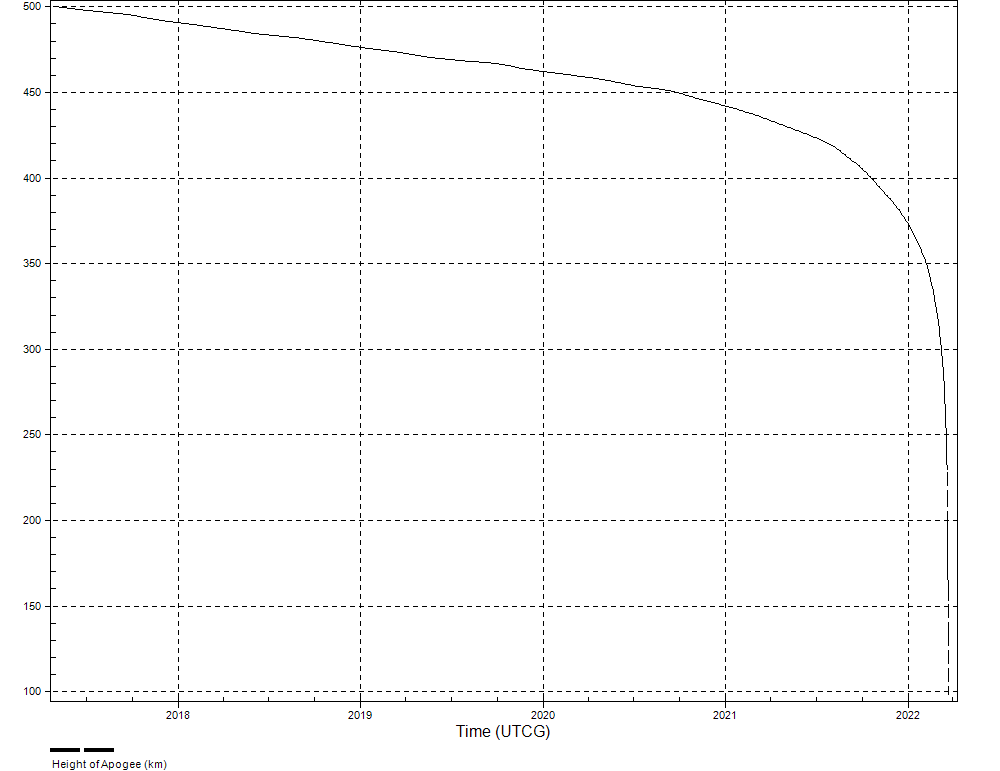
\includegraphics[width = 0.75\textwidth]{chapters/img/receiverDecay.png}
\caption{Receiver satellite orbit decay from a primary orbit with an assumed mission start in March 2017. Values used: $C_D = 2.22$, $mass = 14.92 kg$, $area = 0.3 m^2$.}
\label{fig:recLife}
\end{figure}

\begin{figure}[ht!]
\centering
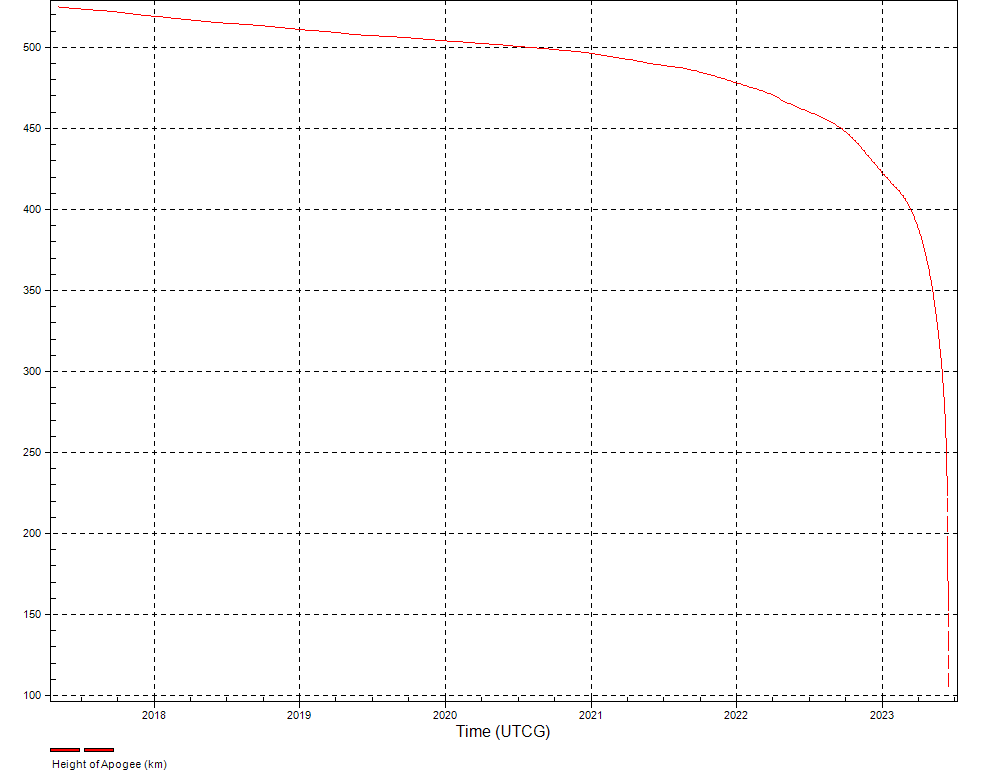
\includegraphics[width = 0.75\textwidth]{chapters/img/receiverDecay2nd.png}
\caption{Receiver satellite orbit decay from a secondary orbit with an assumed mission start in March 2017. Values used: $C_D = 2.22$, $mass = 14.92 kg$, $area = 0.3 m^2$.}
\label{fig:recLife2}
\end{figure}

\subsection{Swarm Configuration}
\label{frSSSC}

The general configuration of all the satellites has been presented in the previous section and can be reviewed in figures \ref{fig:confmax} and \ref{fig:confmin}. As explained, the general rule of separation is 2.18 degrees between the nodes of the different orbital planes and a 2.18 degree in-track phase offset for the satellites occupying the same orbit. 

\begin{figure}[!h]
\centering
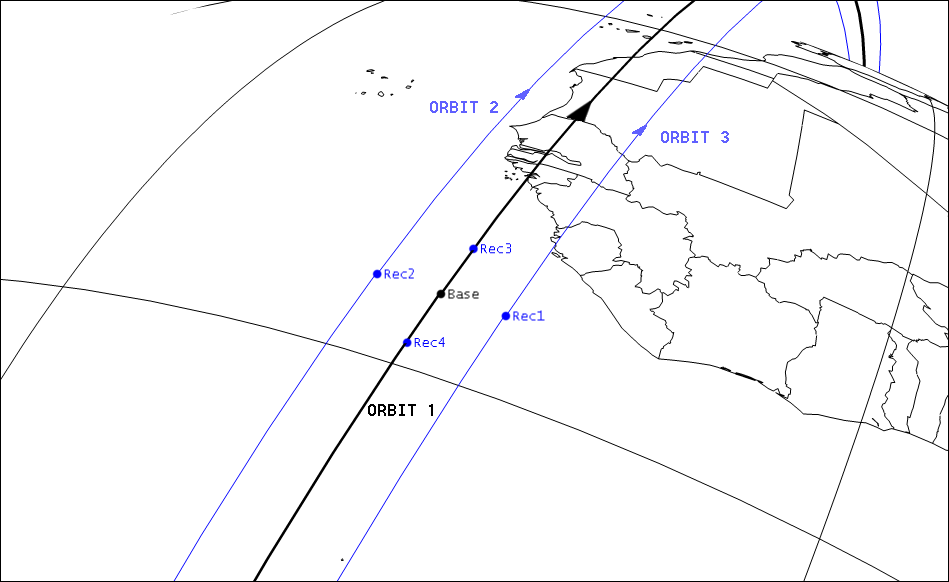
\includegraphics[width=0.8\textwidth, angle=0]{chapters/img/primaryconfmax.png}
\caption{Swarm configuration as seen when the emitter (labeled here as Base) crosses its ascending node. Orbit numbers represent the different orbital planes.}
\label{fig:confmax}
\end{figure}

\begin{figure}[!h]
\centering
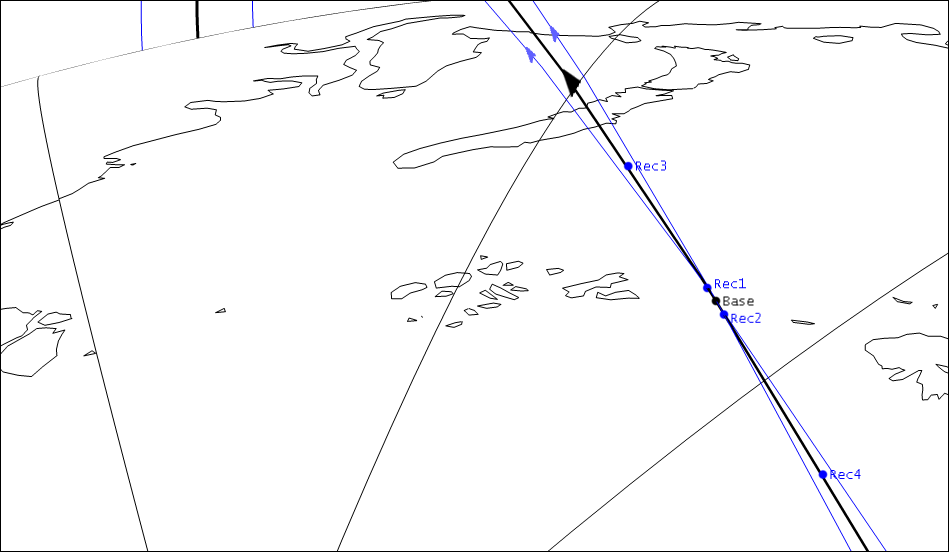
\includegraphics[width=0.8\textwidth, angle=0]{chapters/img/primaryconfmin.png}
\caption{Swarm configuration as seen when the orbit planes intersect. In this figure the intersection in ascent is pictured.}
\label{fig:confmin}
\end{figure}

A representative ground track can be seen in figure \ref{fig:ground} on page \pageref{fig:ground}.

From this general configuration several interesting parameters about the formation can be acquired. Please refer to figure \ref{fig:constgeo} for a general configuration of geometry for constellations with the same inclinations.

\begin{figure}[!h]
\centering
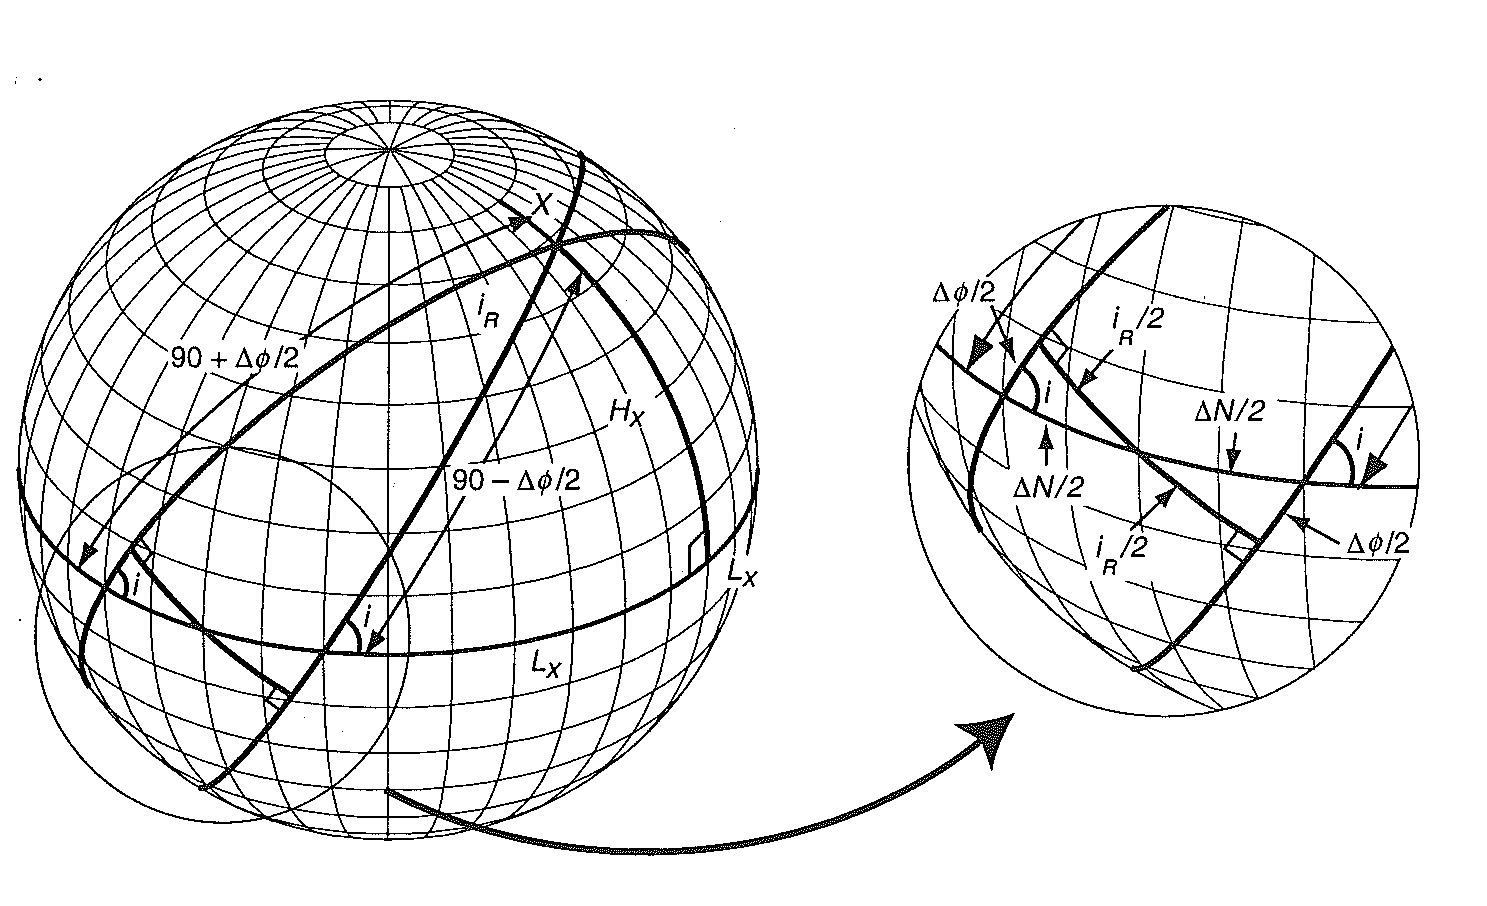
\includegraphics[width=0.8\textwidth, angle=0]{chapters/img/intersectionPhase.png}
\caption{Relative geometry between two orbital planes with the same inclination. \emph{Source: \cite{constDesign}}.}
\label{fig:constgeo}
\end{figure}

The large-scale relative motion of two satellites in different orbits is governed by only two key variables: the relative inclination, $i_R$ and relative phase, $\phi_R$. The relative inclination is the angle at which the two orbit planes intersect. The relative phase is the angle between the satellites when one intersects the other's orbit. The relative phase is the angular separation of the satellites at the time they intersect each other's orbit plane. This happens four times per orbit. The values of these angles are calculated using the following relations:

\begin{equation}
cos i_R = cos^2i+sin^2i cos \Delta N
\label{ir}
\end{equation}
\begin{equation}
\phi_R = (T_2-T_1)n+ \Delta \phi
\label{phir}
\end{equation}
where
\begin{equation}
\Delta \phi = 180 - 2 \phi
\label{deltaPhi}
\end{equation}
\begin{equation}
tan \phi = \frac{tan ( 90 - \Delta N / 2)}{cos i}
\label{tanphi}
\end{equation}

$\Delta N$ is the angular separation at the ascending nodes. Using these equations the relative inclination between Orbit 1 and 2, and 3 and 1 is 2.17 degrees; this corresponds to a separation at the nodes of 261.78 km. The relative inclination between Orbit 2 and 3 is twice this value. The relative phase between the Base and Receiver 1 is 0.1901 (or 22.82 km) as Receiver 1 always crosses Orbit 1 before the emitter satellite. Receiver 2 has the same relative phase with the emitter and trails behind on intersections. The relative phase between satellites in Orbit 2 and 3 is 0.3803 degrees or around 44.6 km.

It is also possible to calculate the maximum and minimum separation angles, $\lambda$, using the following relations:

\begin{equation}
sin ( \frac{\lambda_{min}}{2} ) = sin ( \frac{ \phi_R }{2} ) cos ( \frac{i_R}{2} )
\label{lambdamin}
\end{equation}

\begin{equation}
cos ( \frac{\lambda_{max}}{2} ) = cos ( \frac{ \phi_R }{2} ) cos ( \frac{i_R}{2} )
\label{lambdamax}
\end{equation}

The maximum and minimum angular separation between any two closest orbital planes then becomes 2.1809 and 0.1901 degrees respectively. The nadir angle can also be calculated. This is the angle between the vector pointing to any other satellite and the Earth center vector. The relations are as following:

\begin{equation}
sin (\eta_{min} ) = cos(\lambda _{max}/2) = cos(\phi _R/2)cos(i_R/2)
\end{equation}

\begin{equation}
cos(\eta_{max} ) = sin(\lambda _{min}/2) = sin(\phi _R/2)cos(i_R/2)
\end{equation}

The actual values between cross-track satellites are then 89.91 and 88.91 degrees for maximum and minimum respectively. Along-track satellites have a constant nadir angle of 88.91 degrees.

All these values are enough to simulate along and cross-track relative motion between the various satellites. Figure \ref{fig:relMotion} demonstrates the simulation of large scale relative motion between the Base, Receiver 1 and Receiver 2. Small scale motion is not simulated in this report and requires a more accurate analysis at a later point in time.

\begin{figure}
  \centering
  \subfloat[]{\label{fig:relRec1}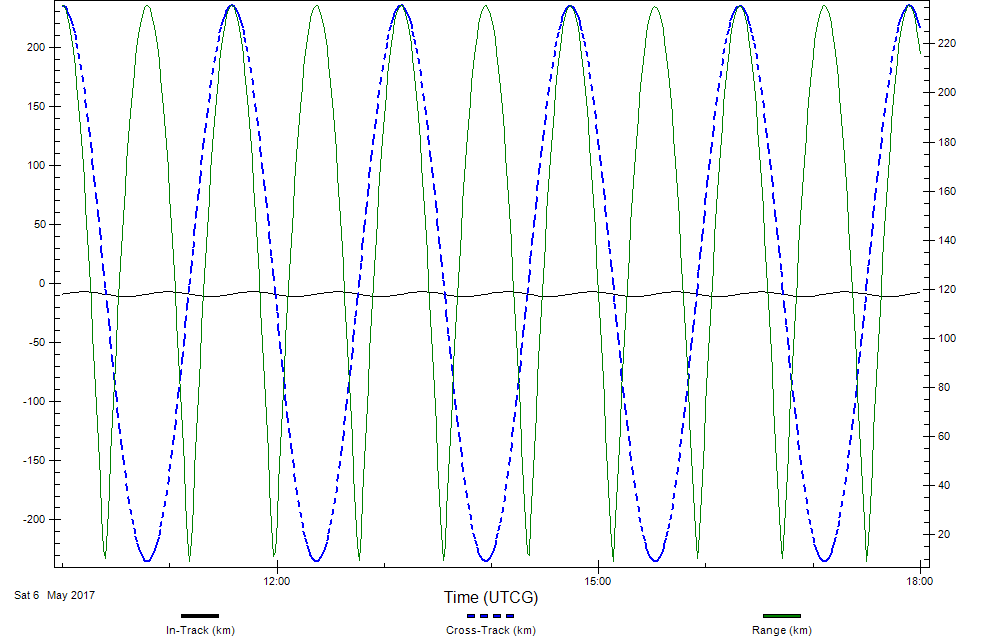
\includegraphics[width=0.9\textwidth]{chapters/img/relRec1.png}}\\                
  \subfloat[]{\label{fig:relRec2}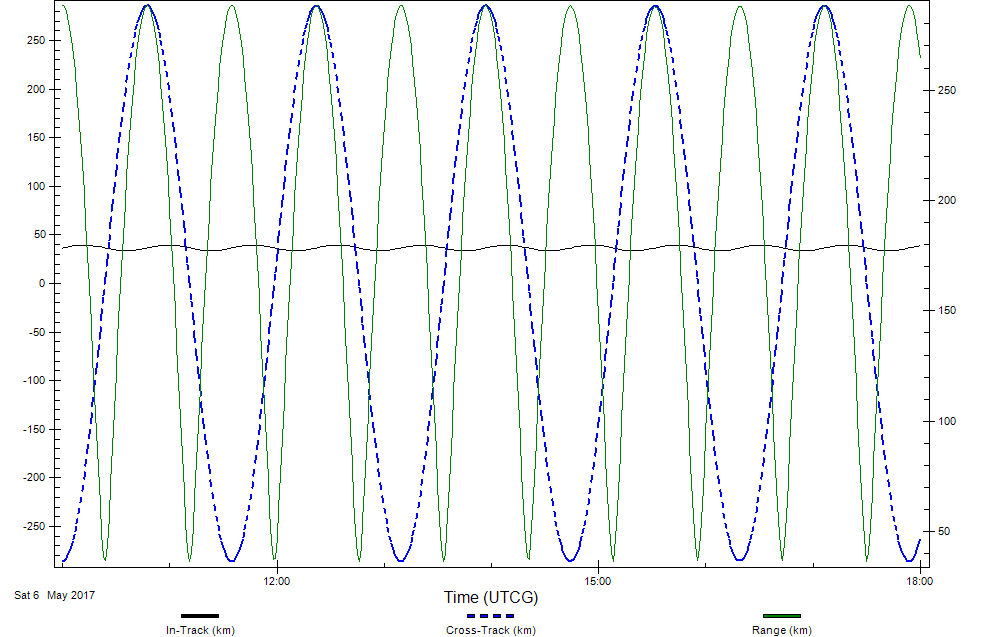
\includegraphics[width=0.9\textwidth]{chapters/img/relRec2.png}}
  \caption{Large scale relative motion (a) of Receiver 1 w.r.t. Base and (b) of Receiver 2 w.r.t. Base.}
  \label{fig:relMotion}
\end{figure}

Finally, to confirm that all orbits intersect at different points, the longitude shift $L_x$ and the latitude $H_x$ of the intersection points are computed using the following equations:

\begin{equation}
L_x = 90 - \Delta N/2
\end{equation}

\begin{equation}
tan H_x = cos\frac{\Delta N}{2}tan i
\end{equation} 

It is only interesting to see the intersections between Base, Receiver 1 and Receiver 2 as these distances are quite small (demonstrated previously to be around 22.82 km). As they all cross the ascending node at the same time the intersection of Receiver 1 will occur first at a longitude offset of 88.9096 degrees and a latitude of 85 degrees w.r.t. the node of the emitter satellite. The intersection of Receiver 2 then occurs at an offset of 91.0896 degrees w.r.t. to the emitter node. The latitude remains the same.

Since the altitude of the orbits does not affect these angles, the relations hold for orbits 1S, 2S and 3S as well.

\subsection{Stationkeeping}
\label{frSSStation}

As mentioned in section \ref{frRecDV} the satellites will not require any $\Delta V$ for stationkeeping maneuvers. This is because the concept of differential drag will be used to minimize propellant and to make the ballistic coefficients of the satellites more consistent.

The principle works in the following way: the satellites are maintained by following the slowest decaying one. This is known as relative stationkeeping. All the satellites are allowed to decay naturally in sync with that single reference. Since the orbits of every satellite are always known due to accurate navigation, it is possible to analyze decay rates. The satellites are then ordered to adjust the orientation of the solar arrays during eclipse in such a way that differential drag reinstates them into the right positions. This is further made possible due to the fact that not position acquisition but rather position knowledge (and thus correct instrument pointing) is of primary importance to data collection.

This concept has been successfully demonstrated by the ORBCOMM satellites \cite{constDesign}. It is understandable that the process of relative stationkeeping is more difficult to manage, however automated systems and prediction models can be designed to deal with this issue. Such systems however are not discussed here.  

\subsection{Collision Avoidance}
\label{frSSCA}

Collision avoidance is an integral part of formation design, yet this analysis cannot be properly performed without the detailed design of the constellation. However some design approximations can be already made to estimate the risks.

In the context of this formation, collision avoidance is important for two reasons: potential loss of two vehicles in a collision, one of them possibly being the emitter, and creation of a debris field which can jeopardize the safety of the rest of the platforms. A debris field evolution can be seen in figure \ref{fig:debris} on page \pageref{fig:debris}. This kind of debris propagation can very quickly lead to a snowball effect and destroy the whole constellation. A NASA90 debris flux model was run to simulate the propogation of a possible collision. The results can be seen in figure \ref{fig:debrisModel} on page \pageref{fig:debrisModel}. 

\begin{figure}[ht!]
  \centering
  \subfloat[]{\label{fig:elecMax}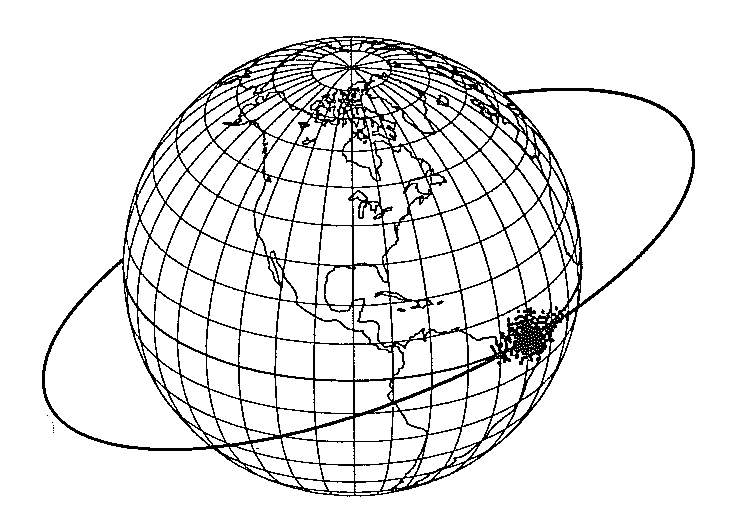
\includegraphics[width=0.4\textwidth]{chapters/img/collA.png}}                
  \subfloat[]{\label{fig:elecMin}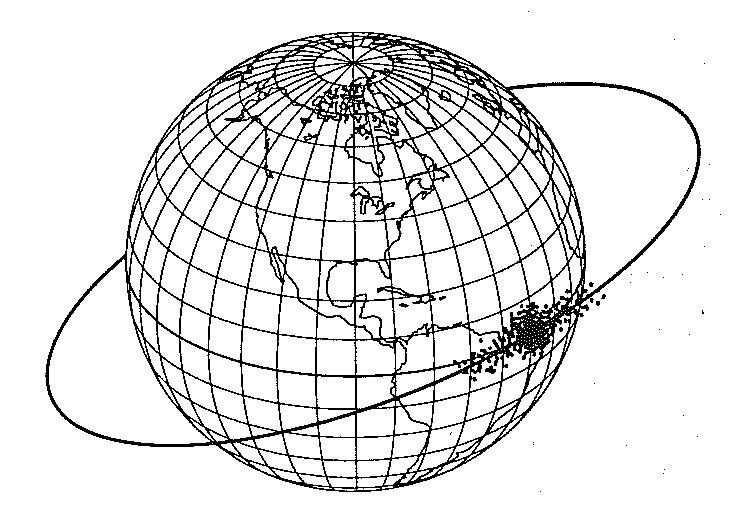
\includegraphics[width=0.4\textwidth]{chapters/img/collB.png}}\\
  \subfloat[]{\label{fig:elecMin2}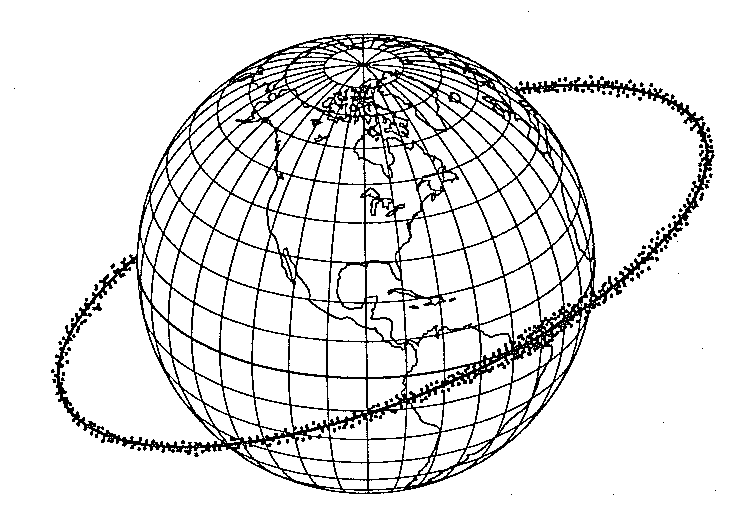
\includegraphics[width=0.4\textwidth]{chapters/img/collC.png}}
  \caption{Debris field evolution, (a) immediately after impact, (b) spreading out after some time and eventually settling into the orbit (c) and decaying. \emph{(Source: \cite{constDesign}})}
  \label{fig:debris}
\end{figure}

\begin{figure}[!h]
\centering
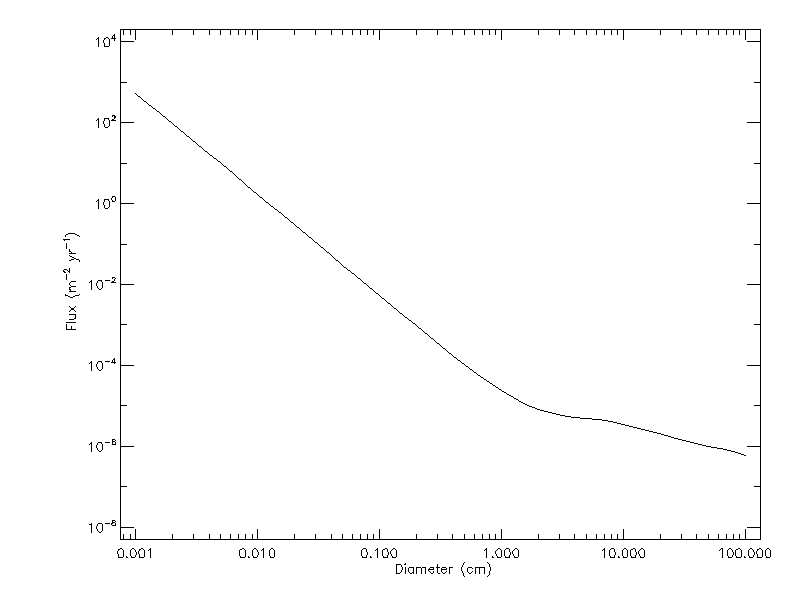
\includegraphics[width=0.5\textwidth, angle=0]{chapters/img/debris.png}
\caption{NASA90 Debris Flux simulation. Orbital altitude - 500 km, Epoch start date - May 2017. \emph{(Source: SPENVIS}.)}
\label{fig:debrisModel}
\end{figure}

Some preliminary formation collision estimates are shown in table \ref{table:coll} on page \pageref{table:coll}.

\begin{table}
	\centering
	
		\begin{tabular}{p{5cm}|p{5cm}|p{5cm}}
		\toprule
	\textbf{Parameters} & \textbf{5 Satellite Formation in 3 Planes} & \textbf{4 Satellite Formation in 3 Planes} \\
		\hline \hline
		No. of satellites & 5 & 4 \\
		No. of orbit planes & 3 & 3 \\ 
		Vertical dispersion [km] & 1 & 1 \\
		In-track dispersion [km] & 22.78 - 276 & 45.56 - 552 \\
		Potential impact area [km$^2$] & 10 & 10 \\ 
		Collision opp. per orbit & 20 & 16 \\
		Orbit period [min] & 94.62 & 95.12 \\ 
		Collision opp. per year & 1.1$*$10$^5$ & 4.0$*$10$^5$ \\
		Collision opp. in 5 years & 5.6$*$10$^5$ & 2.0$*$10$^6$ \\
		Collision prob. per opp. & 1.0$*$10$^{-7}$ & 1.0$*$10$^{-7}$ \\
		Mean number of collisions per year & 0.011 & 0.04\\
		\bottomrule
			\end{tabular}
	\caption{Inter-satellite collision estimations for a formation of 5 primary and 4 secondary satellites. Probability values based on extrapolation of values given in \cite{constDesign}.}
	\label{table:coll}
\end{table}

In order to successfully implement a safety-conscious formation design the following rules will have to be followed:
 
\begin{enumerate}
	\item Maximize spacing between platforms on orbit crossing.
	\item Remove satellites at end of life.
	\item Keep tracking the motion of "dead" satellites.
	\item Remove launcher upper stages from the orbits.
	\item Design replacement injections with collision avoidance in mind.
	\item Capture any ejected components.
	\item Avoid self-detonation.
\end{enumerate}
 
Following these rules will lead to a safer formation and eventually to an extended mission lifetime.

Another topic is collision avoidance of object that are outside the considered formation. That is with other satellites, artificial and natural bodies. Figure \ref{fig:meteor} on page \pageref{fig:meteor} demonstrates a plot of the Grun model of meteoroid flux for 500 km altitude.

\begin{figure}[ht!]
\centering
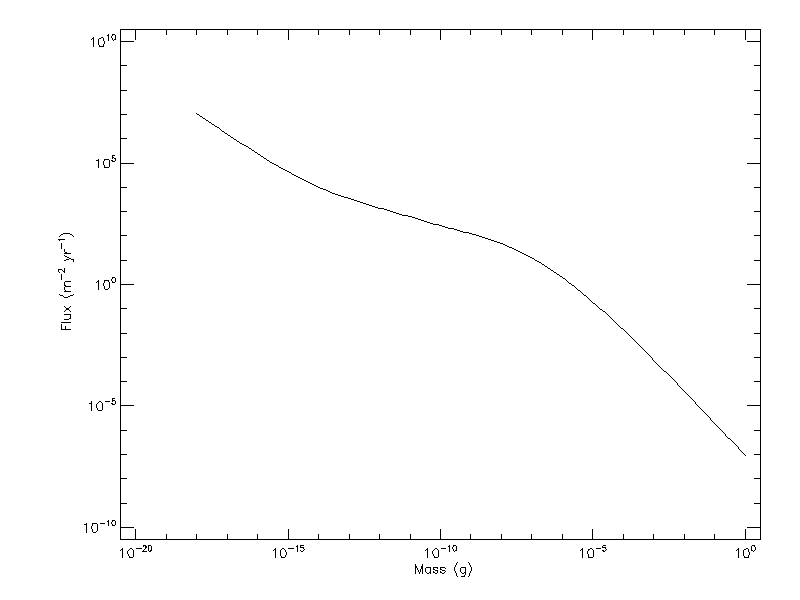
\includegraphics[width = 0.5\textwidth]{chapters/img/meteoroid.png}
\caption{Grun model meteoroid flux for an orbit of 500 km altitude. \emph{Source: SPENVIS}. }
\label{fig:meteor}
\end{figure}

It is obvious that the constellation faces quite a challenge as the low mass of the satellites makes them quite susceptible to objects with a mass of over 1 gram. It is also a problem because only pieces of about 10 cm across and more can be effectively tracked from Earth.

Pending further investigation it is not unreasonable to allow a safety margin of 5\% on the total $\Delta V$ of both satellites. This however is something better left for further investigation.

\section{Space Environment and Shielding}
\label{frSEaS}

In space, satellites are exposed to streams of highly energetic charged particles coming from the sun. Radiation from these particles can cause severe damage to satellite subsystems, including the payload. The main particle radiation source encountered by the swarm in the \ac{LEO} comes from the Van Allen Belts. These are regions around the Earth where charged particles (protons, electrons and ions) are trapped inside the magnetic field of the planet.

The total radiation dose consists of three components: proton dose, electron dose and the so-called Brehmsstrahlung X-Ray dose produced by the interaction between the electrons and the shielding material of the satellite. In \ac{LEO}, energetic protons in the inner radiation belt contribute most to the total radiation dose. This total is also strongly linked to the orbital altitude and below 1000 km will increase at approximately by the 5\textsuperscript{th} power of the altitude. Furthermore, just like with atmospheric drag, the solar activity plays a major role, thus all cases will be examined.

The number of particles trapped in the Van Allen belts in the vicinity of the orbit under question can be modeled using The Space Environment Information System (SPENVIS) that can be located at the following address: \emph{http://www.spenvis.oma.be/}. SPENVIS contains a large array of NASA and ESA (as well as other) tools and models for complex orbit analysis. For the purposes of this evaluation two models are used: AP-8 and AE-8. The first model predicts proton flux with energy levels above 100 MeV. The latter estimates the flux of electrons with energy levels of 0.5 MeV or above.

Figure \ref{fig:elecFlux} on page \pageref{fig:elecFlux} illustrates the trapped proton and electron flux as a function of distance from Earth Center. For the considered altitudes of 300 to 525 km (1.047 to 1.078 Earth radii) the satellites would encounter relatively the same order of magnitude of proton radiation. The electron radiation will decrease as the satellites decay.

It is further possible to estimate the total dose of radiation that the satellites will experience with an assumed aluminum thickness of 1mm. Another SPENVIS model, called SHIELDOSE-2, is used for this estimation. The results are presented in figure \ref{fig:dose}.

From the figure it is seen that with the standard cubesat shielding of 1 mm the total mission exposure is approximately in the order of $10^4$ rad. This is an acceptable range for all space rated instruments considered in this design (Source: \cite{larson}). However if new technologies cannot withstand this dose, an increase of thickness to 1.5 mm would bring the total dose to $10^3$ rad. 

\begin{figure}[!h]
\centering
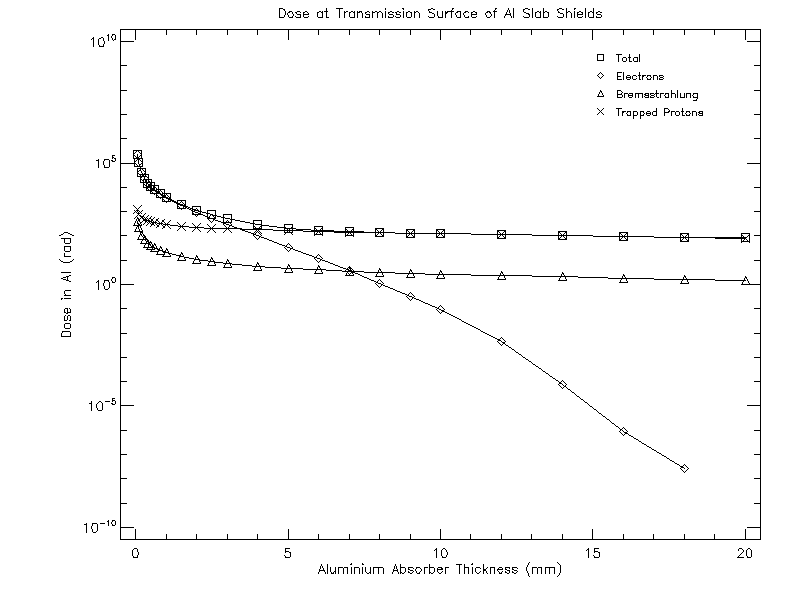
\includegraphics[width = \textwidth]{chapters/img/sd2_dose.png}
\caption{Total radiation dose based on a five year mission at a 500 km altitude. \emph{Source: SPENVIS}. }
\label{fig:dose}
\end{figure}

\begin{figure}
  \centering
  \subfloat[]{\label{fig:elecMax2}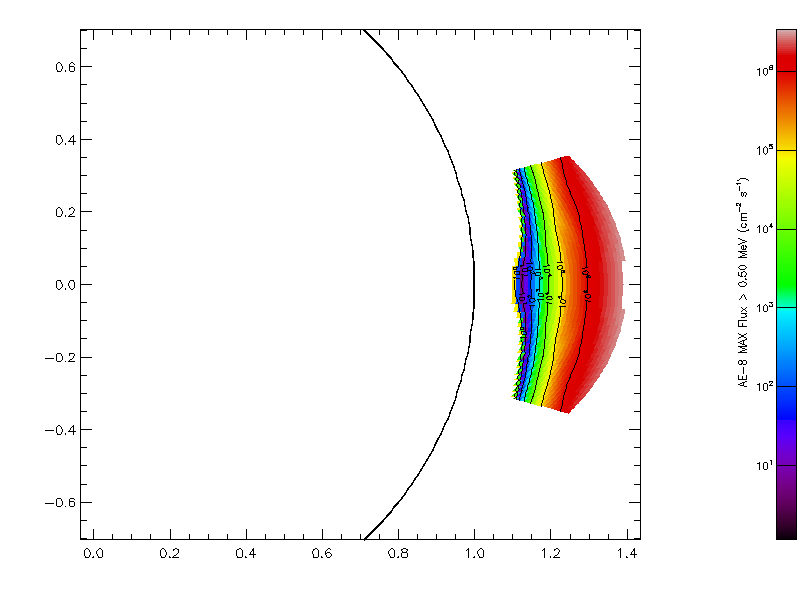
\includegraphics[width=0.7\textwidth]{chapters/img/elecFluxMax.png}}\\                
  \subfloat[]{\label{fig:elecMin3}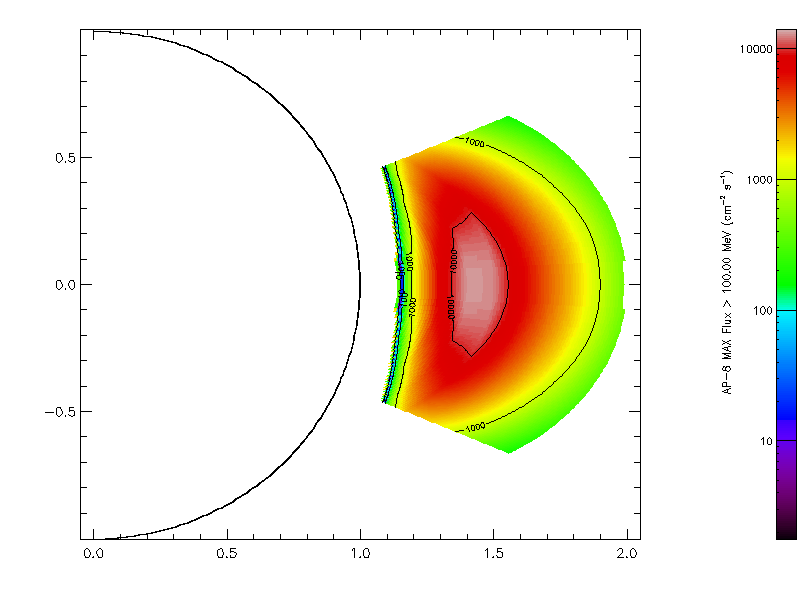
\includegraphics[width=0.7\textwidth]{chapters/img/protFluxMax.png}}
  \caption{AE-8 Electron Flux Model (energy $>$ 0.5 MeV) (a) and AP-8 Proton Flux Model (energy $>$ 100 MeV)(b).}
  \label{fig:elecFlux}
\end{figure}
 

%%%%%%%%%%%%%
%
%      EMITTER				 
%
%%%%%%%%%%%%%

\chapter{Emitter Satellite}
\label{chap:emitter}
This chapter contains the detailed design of the emitter satellite. Each section contains the final design of a different subsystem. 
\\\\
The most important subsystem is the optical emitting payload which can found in section \ref{sec:DDlaser}. The navigation and satellite position is discussed in section \ref{NaviEmitter}. Thirdly the inter-satellite and space-ground communication is explained in detail in section \ref{sec:comm_emitter}. Section \ref{emDDadcs} contains the detailed design of the \ac{ADCS}. The power generation and the corresponding power system is documented in section \ref{emitter_EPS}. The emitter satellite also has a \ac{SPAD} instrument. The details can be found in section \ref{sec:DDreceiver}.
\\\\
Figure \ref{fig:emitterSat} shows an impression of what the emitter satellite will look like.

\begin{figure}
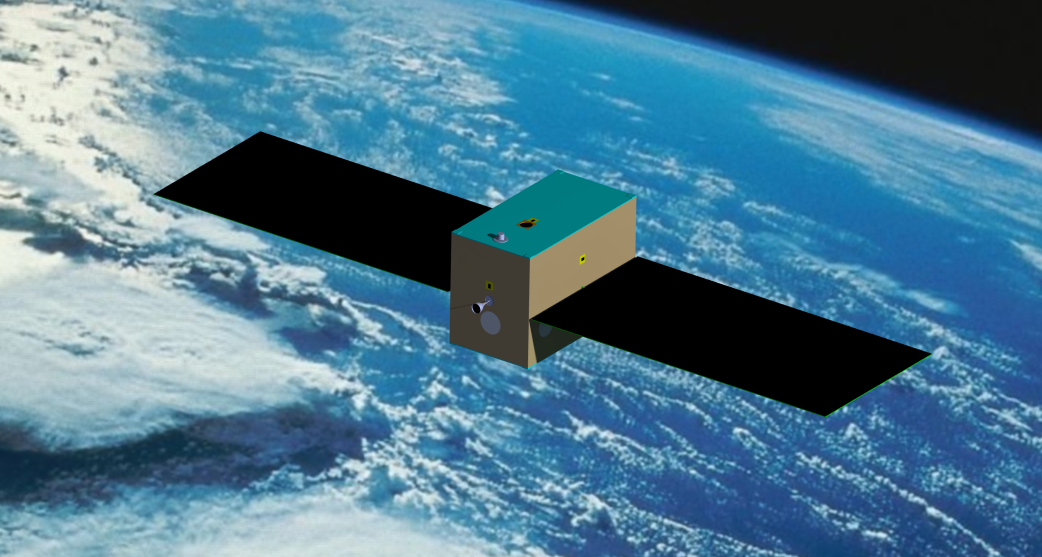
\includegraphics{chapters/img/emitter.png}
\caption{Impression of the emitter satellite}
\label{fig:emitterSat}
\end{figure}
%\section{Detailed Design Optical Emitting Payload} 
\label{sec:DDlaser}
\acs{LiDAR} is a remote sensing system comprising an optical emitting device, used to acquire topographic data, e.g. surface elevation gradients or ground composition by evaluating the \acs{BRDF}, considering multi-angular measurement are taken. For the generation of optical pulses, a highly efficient, diode-pumped, solid-state Nd-YAG \acs{laser} is considered $\left(\ac{DPSSL}\right)$. Solid-State \acp{laser} have a high \acs{TRL} with relatively good properties in terms of beam quality (Q-factor), efficiency and pulse manipulation. Data products for topographical missions require that the \ac{laser} wave form be nearly pure Gaussian (known as transverse resonator mode $TEM_{00}$, both temporally and spatially, with a uniform wave front. The digitized time of flight waveform returning provides the topographic structure \cite{nd_yag_life}.

\subsection{Principles of \textit{AlGaAs} Laser Diodes}
\label{laser_diodes}
\acs{laser} diodes are electrically pumped semiconductor \acp{laser}, in which the gain is generated by an electrical current flowing through a \textit{p-n junction} or (more frequently) a \textit{p-i-n structure}\cite{lasertech}. In such a heterostructure, excitons dynamics can occur (electrons and holes can recombine), releasing the energy portions as photons. This process can be spontaneous, but can also be stimulated by incident photons, in effect leading to optical amplification. Most higher-power \acs{laser} diodes, however, exhibit a relatively poor beam quality, combined with other non-favorable properties, such as a large beam divergence, high asymmetry of beam radius and different \textbf{k}-vector beam quality , and astigmatism (property of rays to exhibit different foci in different symmetrical planes). Especially considering the long distances used in \acs{LiDAR} missions, these properties degrade the potential data quantity, as well as quality. The basic diode \acs{laser} configuration can be found in figure \ref{diode_laser_configuration} on page \pageref{diode_laser_configuration}.

\begin{figure} [ht]
\centering
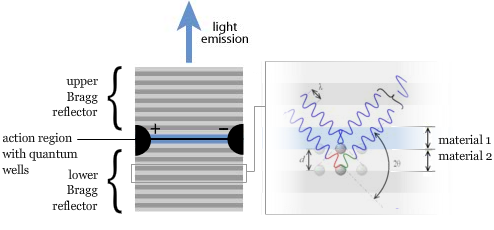
\includegraphics[scale=0.6]{chapters/img/diodelaser.png}	
\caption[Basic diode laser configuration]{Basic diode laser configuration \cite{laser_power}. Each layer boundary causes a partial reflection of an optical wave. For waves whose wavelength is close to four times the optical thickness of the layers, the many reflections combine with constructive interference, and the layers act as a high-quality reflector. The range of wavelengths that are reflected is called the \textit{photonic stopband}. Bragg's law describes the condition for constructive interference from successive crystallographic planes of the crystalline lattice according to n $\lambda  =2d\cdot sin(\theta)$.}
\label{diode_laser_configuration}
\end{figure}

A quantum well, used in diode lasers, is a thin layer which can confine (quasi-)particles (typically electrons or holes) in the dimension perpendicular to the layer surface, whereas the movement in the other dimensions is not restricted. A quantum well is often realized with a thin layer of a semiconductor medium, embedded between other semiconductor layers of wider bandgap. The thickness of such a quantum well is typically $\sim$5 - 20 nm. 

A major challenge is to reach the laser threshold, because the optical gain for the intracavity laser beam occurs only on a very small distance (in one or several quantum wells). It is therefore necessary to realize a laser resonator with very low losses, i.e., \textit{Bragg mirrors} with high reflectivity. A Bragg mirror (also called \textit{distributed Bragg reflector}) is a structure which consists of an alternating sequence of layers of two different optical materials. The principle of operation can be understood as follows. Each interface between the two materials contributes a Fresnel reflection. For the design wavelength, the optical path length difference between reflections from subsequent interfaces is half the wavelength; in addition, the reflection coefficients for the interfaces have alternating signs. Therefore, all reflected components from the interfaces interfere constructively, which results in a strong reflection. The reflectivity achieved is determined by the number of layer pairs and by the refractive index contrast between the layer materials. 

Individual \acs{laser} diodes normally generate quasi-continuous waves with powers $\sim$ 1 - 10 mW. To be able to generate higher power ($\sim$1 - 10 W) \textit{laser diodes arrays} or \textit{laser diode stacks} can be created, simply be combining multiple individual \acs{laser} diodes. High-power \acp{LDA} are used for a variety of space-based remote sensor laser programs as an energy source for \acp{DPSSL}. \acp{LDA} have been flown on NASA missions including MOLA, GLAS and MLA and have continued to be viewed as an important part of the \acs{laser}-based instrument component suite \cite{lda_main}. 

Laser diode bars have many single emitters arranged side-by-side and spaced approximately 0.5 mm apart, on a single slab of semiconductor material measuring approximately 0.5 mm x 10 mm in size. The individual emitters are connected in parallel which keeps the required voltage low at $\sim$2 V, but increases the required current to $\sim$50 A/bar to 100 A/bar. Stacking these laser diode bars 2 to 20+ slabs high yields high power \acp{LDA} capable of emitting several hundreds of Watts. Electrically, the bars are wired in series increasing the voltage by 2 V/bar while maintaining the total current at $\sim$50 A to 100 A. These arrays are one of the enabling technologies for efficient, high power solid-state lasers.

Traditionally these arrays are operated in QCW (Quasi Continuous Wave) mode with pulse widths of $\sim$50 $\mu$s to 200 $\mu$s and repetition rates of $\sim$10 - 200 Hz. In QCW mode, the wavelength and the output power of the laser reaches steady-state, but the temperature does not. The advantage is a substantially higher output power than in CW mode, where the output power would be limited by the internal heating and the heat sinking properties of the device. The disadvantage is a much higher thermally induced mechanical stress caused by the constant heating and cooling cycle of the QCW operational mode, considering non-conductive cooling configurations.

Considering the fact that Nd:YAG is considered as gain medium (\ref{nd_yag}), the existence of strong $Nd^{3+}$ absorption near 808 nm permits efficient pumping with a GaAlAs (Gallium-Aluminium-Arsenide) diode \acp{laser} for the $F_{3/2}\rightarrow I_{9/2}$ transition. The direct band gap crystal AlGaAs is often used for laser diodes with wavelengths between
750 nm and 880 nm. $Al_{x}Ga_{1-x}As$, through changing the x, the ratio of the aluminum
to gallium can be adjusted to vary the band gap and thereby control the wavelength. In the double heterostructure, stimulated emission occurs only within a thin active
layer of GaAs, which is sandwiched between p- and n- doped AlGaAs layers that have
a wider band gap. Laser diodes use hetero junctions to achieve simultaneous carrier and photon confinement in the active region. The basic AlGaAs diode \acs{laser} configuration can be found in figure \ref{algaas_laser_configuration} on page \pageref{algaas_laser_configuration}.

\begin{figure} [ht]
\centering
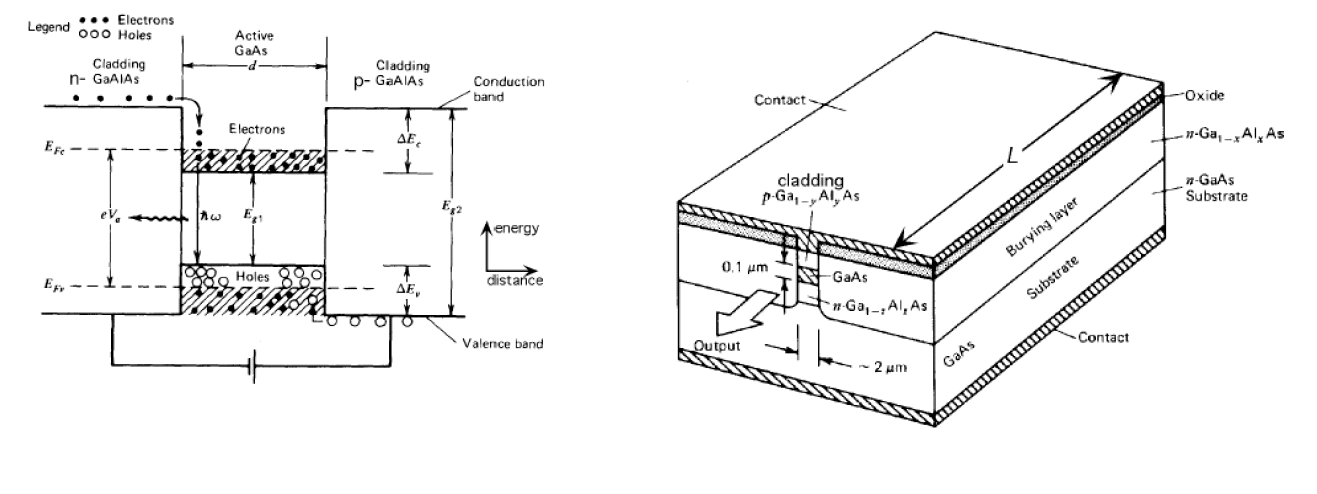
\includegraphics[scale=0.5]{chapters/img/laser_diode_algaas.png}	
\caption{Basic AlGaAs diode \acs{laser} configuration \cite{algaasdiodes}. Left: Exciton dynamics initialize after applying electrical field.}
\label{algaas_laser_configuration}
\end{figure}

A high laser efficiency demands that the light and injected charge carriers be confined as closely as possible to the same volume. The AlGaAs daser diode consists of a double heterojunction formed by an undoped (or lightly p-doped) active region surrounded by high bandgap p and n $Al_{x}Ga_{1-x}As$ cladding layers \cite{algaasdiodes}. The surrounding cladding layers provide an energy barrier to confine carriers to the active region. The actual operation wavelengths may range from 750 $\sim$ 880 nm due to the effects of dopants, the size of the active region, and the compositions of the active and cladding layers. When a certain parameter is fixed, the wavelength can vary in several (sub)nanometers due to other variables. For example, when the active layer has an energy gap $E_{g} = 1.424 eV$, the nominal emission wavelength is $\lambda = hc/E_{g}= 871 nm$. When a bias voltage is applied in the forward direction, electrons and holes are injected into the active layer. Since the band gap energy is larger in the cladding layers than in the active layer, the injected electrons and holes are prevented from diffusing across the junction by the potential barriers formed between the active layer and cladding layers. The electrons and holes confined to the active layer create a state of population inversion, allowing the amplification of light by stimulated emission. The typical diode laser characteristics can be found in figure \ref{diode_laser_char} on page \pageref{diode_laser_char}.

\begin{figure} [ht]
\centering
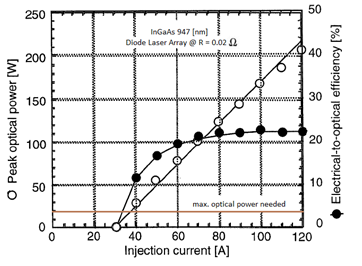
\includegraphics[scale=0.5]{chapters/img/laser_power.png}	
\caption{Typical diode \acs{laser} characteristics; power and current information at constant temperature. Parameters decrease with higher temperatures.}
\label{diode_laser_char}
\end{figure}

\subsection{Diode Pumped Solid-State Laser Configuration} 
\label{laserconfig}

The basic (simplified) configuration of the \acs{laser} with dimensions is shown in figure \ref{laser_dimension} on page \pageref{laser_dimension}. Individual components will be explained later in this section.

\begin{figure} [ht]
\centering
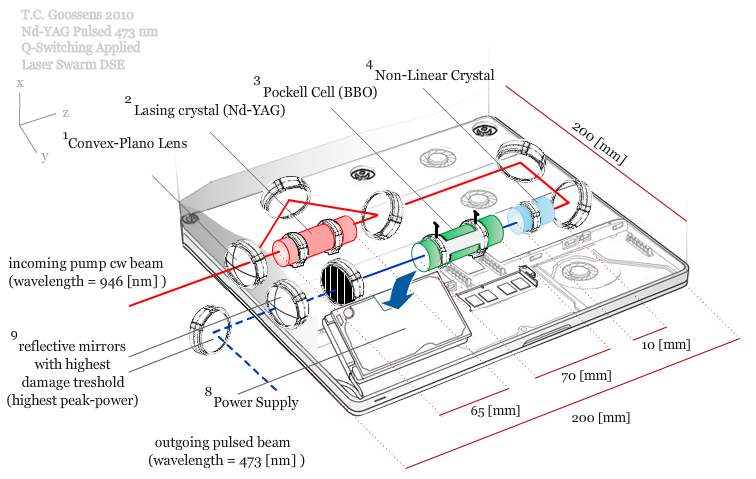
\includegraphics[scale=0.5]{chapters/img/laserconfig.png}	
\caption{Basic (simplyfied) configuration of the \acs{laser} with dimensions.}
\label{laser_dimension}
\end{figure}

\subsubsection{Nd-YAG Laser Characteristics}
\label{nd_yag}
\textit{Yttrium Aluminum Garnet} has emerged as the most widely produced laser gain host and has enjoyed recent popularity as a substrate material for optical components. The YAG host is a stable compound, mechanically robust, physically hard, optically isotropic, and transparent from below 300 to beyond 4,000 nm. YAG single crystals are able to accept trivalent laser activator ions from both the rare Earth and transition metal groups, and can be grown with very low strain. The table \ref{tab:ndyag_parameters} on page \pageref{tab:ndyag_parameters} gives the parameters of the Nd-YAG laser.

\begin{table}[ht!]
\centering
\begin{tabular}{|l|c|}
\hline
  \multicolumn{2}{|c|}{Nd-YAG (Neodymium Yttrium Aluminum Garnet $Y_3Al_5O_{12}$)}\\\hline
  Nd Concentration & 0.2 - 1.4 \% \\
  Diameter & 0.5 - 15.0 mm \\
  Length & 1.0 - 220.0 mm \\
  Damage Threshold & $> 20\ J/cm^2$  \\
  Refractive Index(n) & 1.8169 \@ 1,064 nm \\
  Thermal & 0.129 W/cm.K \\
  Conductivity & \\
  Specific Heat & 0.59 J/g.K\\
  Density & 4.55 $gm/cm^2$\\
  Tensile Strength & 280 MPa \\
  Young's Modulus & 282 GPa\\
  dn/dT & $+8.9\cdot10^{-6}\ K^{-1}$\\\hline
\end{tabular}
\caption{Solide-State laser Nd-YAG parameters}
\label{tab:ndyag_parameters}
\end{table}

For applications where $TEM_{00}$ single mode operation is required, it is necessary to reduce or eliminate the variations in the bulk material and in the absorption of the pumping radiation throughout the component. In addition, wavefront distortions due to geometric imperfections and thermal gradient effects such as thermal lensing must be minimized. In this case, Neodymium concentration in the 0.4 to 0.8\% range is typically specified.

\begin{figure} [ht]
\centering
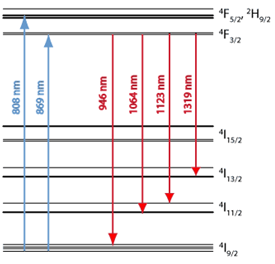
\includegraphics[scale=1.2]{chapters/img/laser_line.png}	
\caption{Quantum energy level and transitions for the Nd:YAG crystal, including the used $F_{3/2}\rightarrow I_{9/2}$ transition.}
\label{laser}
\end{figure}

\subsubsection{Second Harmonic Generation}
\label{SHG}
Since Nd-YAG has no principle absorption peak at the desired wavelength for the \acs{LiDAR} mission, the frequency should be altered from the original 946 [nm]. This can be done using \textit{second harmonic generation} or \textit{frequency doubling} in nonlinear crystals.
The physical mechanism behind frequency doubling can be understood as follows. Due to the ��(2) nonlinearity, the fundamental (pump) wave generates a nonlinear polarization wave which oscillates with twice the fundamental frequency. According to Maxwell's equations, this nonlinear polarization wave radiates an electromagnetic field with this doubled frequency. Due to phase-matching issues, the generated second-harmonic field propagates dominantly in the direction of the nonlinear polarization wave. The latter also interacts with the fundamental wave, so that the pump wave can be attenuated (pump depletion) when the second-harmonic intensity develops: energy is transferred from the pump wave to the second-harmonic wave.
$\beta-BaB_{2}O_{4}$ is used for second, third, fourth and fifth harmonic generation of Nd doping \acp{laser}. Typical dimensions of these crystal are $\sim0.05 - 10\ mm$.

\subsubsection{Pulse Generation}
\label{pockel}
The generation and manipulation of pulses can highly influent the data in \acs{LiDAR} missions. To be able to transform the quasi-continuous wave into a pulsed wave, Q-switching is applied. Q-switching is a technique for obtaining energetic short pulses from a \acs{laser} by modulating the intracavity losses and thus the Q-factor (a measure of the damping of resonator modes) of the laser resonator. The technique is mainly applied for the generation of nanosecond pulses of high energy and peak power with solid-state bulk lasers. For \textit{active Q-switching}, the losses are modulated with an active control element typically either an acousto-optic or electro-optic modulator. Both techniques rely on the fact that the optical properties within a nonlinear crystal on the occurrence of an induced sound wave (acousto-optic) or electric field (electro-optic). There are also mechanical, less viable for space missions, Q-switches such as spinning mirrors, used as end mirrors of laser resonators. In any case, the achieved pulse energy and pulse duration depends on the energy stored in the gain medium, i.e. on the pump power and the pulse repetition rate.  A Pockels cell is a device consisting of an electro-optic crystal including electrodes through which a electromagnetic beam can propagate. Dependent on the configuration, the phase delay or polarization state in the crystal (due to the \textit{Pockels effect}) can be modulated by applying a flux electric voltage (typical second harmonic generation characteristics: $\sim40,000 V / 0.1\ mA$)  Hence, for short periods (dt) the polarization state of the incoming electromagnetic radiation can be altered. If a \textit{polarizer disk} is used after the Pockel cell, the generation of pulses will begin, since the polarizer disk transmits certain polarized states only, deflecting the rest (acting like a 'polarize filter'). Pulses in the order of nanoseconds could be created this way. Care should be taken at the fact that the peak power after the Pockel cell is increased in several orders, due to the conversion from continuous to pulsed waves. Hence, the polarizer disk should be able to cope with these stresses. According to data posted after the GLAS-mission (using the same sort of \acs{laser}, an optical induced layer was formed at the non-linear crystal, probably induced by the high peak powers of the pulsed waves. In this configuration, the pulsed wave is created after the $\beta-BaB_{2}O_{4}$ - crystal, reducing the risk of the creation of critical optical damage (COD). The figure \ref{fig:pockel_cell} on page \pageref{fig:pockel_cell} is the change in polarized state of electromagnetic radiation when passed through a Pockel cell.

\begin{figure} [ht]
\centering
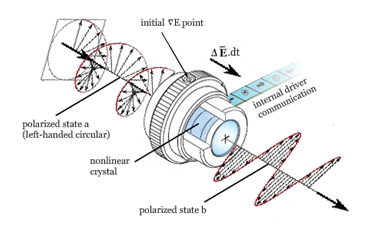
\includegraphics[scale=1.2]{chapters/img/laser_polarized.png}	
\caption[Polarized state passed through a Pockel cell]{Change in polarized state of electromagnetic radiation when passed through a Pockel cell. Communication with Pockel cell driver should be applied to determine magnitude of electric field flux and \textit{dt}. Considering the fact that the value of $f_{rep}$ could be changed in-mission (for example, if the pulse rate should be higher due to lower reflectivity on specific areas) communication with ground-station should be applied.}
\label{fig:pockel_cell}
\end{figure}

\subsection{Optical Characteristics} 
\label{opticalchar}
Considering for a moment, the radius of the beam equals 400 $\mu$m. Considering a $TEM_{00}$ transverse mode of electromagnetic radiation this results in a area equal to 
\begin{equation}
\label{area}
A_{beam} = \pi \cdot r^{2} = \pi \cdot 400^{2} = 502,654\ \mu m^{2} = 0.50265\ cm^{2}
\end{equation}

The pulse energy $E_{p}$ J (maximum optical power of a pulse) is determined using the simulator. Sufficient energy should be present within the electromagnetic radiation to ensure the optimum path from the transmitter towards the receiver. Lowering the value of $E_{p}$ below this threshold energy can lead to atmospheric and surface absorption or translational mismatching due to incorrect scattering. The value of $E_{p}$ of this particular mission is determined to be $\sim$1 mJ (see \ref{chap:sim}).
Pulse repetition rate $f_{rep}$ Hz, i.e. the number of pulses emitted per second, is an important parameter for the altimetry mission. Again, using the results from the simulator, the quantity of this parameter can be determined to be $\sim$5000 Hz ($\Delta$t = 0.0002 s with a pulse duration $t_{p}$ $\sim$10 ns). Using the value of $f_{rep}$, the spatial resolution of the pulses along-track and in the nadir-direction can be calculated, considering the orbital velocity to be fixed at the determined altitude.  
\begin{equation}
\label{alongtrackres}
d_{along} = \Delta t \cdot v = 0.0002\ s \cdot 7,617\ m/s = 1.5234\ m
\end{equation}

\begin{equation}
\label{alongtracknadir}
d_{nadir} = \Delta t \cdot c = 0.0002\ s \cdot 299,792,458\ m/s = 59,958.49\ m
\end{equation}

Considering the value of $E_{p}$ to be 1 [mJ] with a $f_{rep}$ of 5,000 [Hz], the total power that should be induced within the electromagnetic wave can be calculated.
\begin{equation}
\label{outputpower}
P_{output} = E_{p} \cdot f_{rep} = 0.001\ J \cdot 5,000\ 1/s = 5.0\ W
\end{equation}

The \textit{total} electrical-to-optical power efficiency of a laser system ($\eta_{wp}$), i.e. the \textit{wall plug efficiency}, typically is $\sim 10\ \%$, however, linear interpolations of the current data, considering the large amount of research done on this subject, shows that $\eta_{wp}$ increases with one percent point every year (on average) from 2004, giving an wall plug efficiency of $\sim16\ \%$ in 2010 and \textgreater20 \% in 2015 \cite{nd_yag_life}. A higher value of $\eta_{wp}$ reduces the electrical power consumption and also the amount of heat which has to be removed. Simulation shows a power needed for succesfull photon detection in this altimetry mission of $\sim6 W$, ending up with a total power need of 60 W ($\eta_{wp}$=0.1) or (more realistic) 30 W ($\eta_{wp}$ = 0.2). 
  
The pulse peak intensity equals $E_{p}/t_{p} = 0.001\ J / 10\cdot10^{-9} [s] = 100,000\ W$. The intensity turns out to be $\frac{E_{p}/t_{p}}{A_{beam}} = \frac{100,000\ W}{0.50265\ cm^{2}} = 198,950.6\ W/cm^{2} (0.00199\ J/cm^{2}/10ns)$. The standard damage threshold energy $E_{p,damage}$for dielectric components equals $0.5 - 10\ J/cm^{2}/10ns$. Considering the lowest value $I_{p,damage}$, hence, $0.5\ J/cm^{2}/10ns$, and converting this to the appropriate dimensions, shows the intensity created within the electromagnetic pulses should do no harm to the dielectric components. Especially the polarizer disk (with the lowest $I_{p,damage}$) is vulnerable for peak power caused by pulsed electromagnetic radiation. 

\subsection{Gaussian Beam Propagation And Diffraction}
	\label{diffraction}

Collimated plane wave propagation (uniform \textbf{k}-vector distribution) in optical systems would give rise to discrete and accurate calculations. However, due to optical distortions and modifications, the \textbf{k}-vector distribution can change, hence, altering the wave propagation. 

\textit{Gaussian Beams}
The figure \ref{gaussian_beam} on page \pageref{gaussian_beam} showsFor the analysis of the \acs{laser} beam intensity profile, a Gaussian profile (transverse resonator mode $TEM_{00}$) is considered corrected by the $M^{2}$ factor for optical distortion. The $M^{2}$ factor is a common measure of the beam quality of a laser beam.  The electric field distribution for a Gaussian beam is represented as:

\begin{equation}
	E(r,z) = E_{0}\cdot \frac{w_{0}}{w(z)} \cdot exp\left[\frac{-r^{2}}{w(z)}\right]\cdot exp\left[-i(kz-arctan\left(\frac{z}{z_{r}}\right)+\frac{kr^{2}}{2R(z)}\right]
\end{equation}

\begin{equation}
	E(x,y,z) = exp\left[\frac{-i(kz + \psi(z)}{w(z)}\right]exp\left[\frac{-(x^{2}+y^{2})}{w^{2}(z)} - ik \frac{(x^{2}+y^{2})}{2R(z)}\right]
\end{equation}

\begin{figure} [ht]
\centering
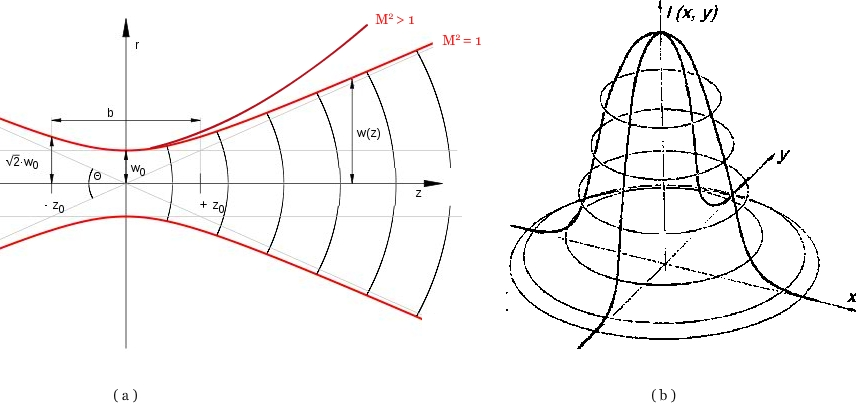
\includegraphics[scale=0.5]{chapters/img/TEM00.jpg}	
\caption{Mathematical description of the Gaussian beam/ $TEM_{00}$ transverse mode.}
\label{gaussian_beam}
\end{figure}

The main point of this section is to determine the Gaussian beam propagations dependency on diffraction phenomenon. To characterize the Gaussian beam in more details, the following equations are used to be able to describe the propagation.

\begin{equation}
\theta = \frac{\lambda}{\pi\cdot w_{0}}
\end{equation}

\begin{equation}
w_{real}(z)=w_{0,real}\sqrt{\left[1 + \left(\frac{z(\theta+\Delta \alpha) M^{2}}{w_{0,real}}\right)^{2}\right]}
\end{equation}

\begin{equation}
R_{real}(z)=z\left[1 + \left(\frac{w_{0,real}}{z\theta M^{2}}\right)^{2}\right]
\end{equation}

\begin{equation}
w_{real}(z)=w_{0,real}(z)\sqrt{\left[1 + \left(\frac{z\lambda M^{2}}{\pi w_{0,real}^{2}}\right)^{2}\right]}
\end{equation}

\begin{equation}
R_{real}(z)=z\left[1 + \left(\frac{w_{0,real}}{z(\theta+\Delta \alpha) M^{2}}\right)^{2}\right]
\end{equation}

\textit{Fraunhofer Diffraction} 
Diffraction is a fundamental characteristic of all wave fields. The effect of diffraction is typically manifested when an obstacle is placed in the path of a beam. On an observation screen some distance away from the obstacle, one observes a rather complicated modulation of the time-average intensity in the vicinity of the boundary separating the illuminated region from the geometrical shadow cast by the obstacle. With the use of high-power lasers, diffraction of radiation beams (cavity oscillating in the fundamental transverse Gaussian $TEM_{00}$ mode) with finite transverse dimensions has significant consequences. The Fresnel number $F = a^{2}/\lambda \cdot R$, where a is the characteristic size ("radius") of the aperture,  $\lambda$ is the wavelength, and R is the distance from the aperture, determines the diffraction regime that should be considered (F$\ll$ 1: Fraunhofer (far-field); F \textgreater 1, Fresnel). The far-field light field is the Fourier transform of the aperatured field. The far-field light field is the Fourier transform of the aperatured field.
	
\begin{equation} 
E(k_{x},k_{y}) = \mathcal{F}\left\{{\overbrace{t(x,y)}^{Transmission\  function}\cdot E(x,y)}\right\} = \iint(exp(-i(k_{x} x + k_{y}y))\cdot t(x,y)\cdot E(x,y)dxdy 
\end{equation} 

\begin{equation}
E(x,y,z) = \frac{exp\left[-i(kz + \psi(z))\right]}{w(z)}\cdot exp\left[\frac{-(x^{2}+y^{2})}{w^{2}(z)}-\frac{ik(x^{2}+y^{2})}{2R(z)}\right]
\end{equation}

The lens incorporates a phase delay to the outgoing electromagnetic field. For the entire derivation of the this equation, \cite{laser_power} should be evaluated. 

\begin{equation}
t_{lens} = exp\left\{-i(\left((n-1)(\frac{k}{2R}(x^{2}+y^{2})\right)\right\}
\end{equation}

Combining the above calculations, calculations for the Fraunhofer diffraction can be conducted, which shows the dependency on divergence.

\begin{equation}
\mathcal{F}\left\{\left(exp\left\{-i\left((n-1)\left(\frac{k}{2R(z)}\right)(x^{2}+y^{2})\right)\right\}\right)\otimes\left(\frac{exp\left[-i(kz + \psi(z))\right]}{w(z)}\cdot exp\left[\frac{-(x^{2}+y^{2})}{w^{2}(z)}-\frac{ik(x^{2}+y^{2})}{2R(z)}\right]\right)\right\}
\end{equation}

A different point of view, conveniently in the sense of the \acs{LiDAR} mission, considers the use of focal lengths to change the Gaussian beam diffraction, giving the same result as the above Fourier transform, i.e. the divergences influence the intensity profile. 

\begin{equation} 
E(x_{1},y_{1})=\iint\left[exp\left( ik\left(\frac{-2x x_{1}-2y y_{1}}{2z} + \frac{x^{2}+y^{2}}{2z}\cdot t_{lens}(x,y)\cdot E(x,y)\right)\right)\right]dx dy
\end{equation} 

Avoiding the quadratic terms and using the following relationship, the Fraunhofer diffraction pattern can be conducted.

\begin{equation} 
\frac{k}{2z}=(n-1)\frac{k}{2R_{1}}
\end{equation} 

Adjusting the lens formula gives:

\begin{equation} 
\frac{1}{f}=\left(n-1\right)\left[\frac{1}{R_{1}}-\frac{1}{R_{2}}\right]
\end{equation} 

The final result shows the dependency of focus length to the Fourier transform of the aperature field. 

\begin{equation} 
E(x_{1},y_{1})=\iint exp\left[-i\frac{k}{f}\left(xx_{1}+yy_{1}\right)\cdot t(x,y)\cdot E(x,y)\right] dx dy
\end{equation}
 
\subsection{Thermal Control} 
\label{opticalthermal}
Basically, there are three critical parts (\acs{LDA}, Nd:YAG \acs{laser} crystal and optical components after polarizer disk) of the \acs{laser} configuration in terms of thermal control. All of these components shall be considered in this subsection.

\textit{\acs{LDA}}.
The constituent parts and materials of a typical \acs{LDA} are the diode die (laser bar) and the mechanical structure. The packaging design and materials enable the array of laser bars to stay together in a stack, to be energized electrically (with a relatively high drive current), to pass the heat generated out of the unit to the mounting surface (thermal path, heat sinking), to be sufficiently rugged against mechanical insults, to provide a standard mounting interface (screws or clamps) and to be as small as possible. The active region of the \acs{LDA}, where heat is generated, is only about 1 micron wide, located about 3 microns from the P-side of the bar. The bars are about 0.1 mm wide and typically spaced about 0.5 mm from each other. Waste energy in the form of heat must be conductively transferred into the solder material and from there into the heat sink material (typically BeO or CuW) as rapidly as possible. The solder material of choice is a soft Indium alloy for its ductile property allowing the bar and the heat sink to expand or contract at different rate with temperature. The \acs{LDA} manufacturers try to use materials which possess higher thermal conductivity and a relatively comparable coefficient of thermal expansion (CTE) in order to minimize the thermal resistance of the device and the induced mechanical stresses. Additionally important to reducing mechanical stress is consideration of the use of soft solders which are highly pliable with a relatively low melting point (\~ 160 $C^{\circ}$). Post life test analysis indicates that solder deformation caused solder roll-over, in turn creating voids, which increase thermal resistance. When coupled with built-in stress due to fabrication, such roll over, in time often obstructs emitters, leading to increased heating, or extends across the bar from anode to cathode causing bar shorts which eventually result in contaminations to the emitter face and localized hot spots, further degrading performance. Excessive heating and thermal cycling of the \acs{LDA} active regions plays a key role in limiting the reliability and lifetime of \acp{LDA} operated in the QCW mode, particularly where pulse widths are long. To improve the assembles heat extraction performance, advanced materials are being considered for packaging \acp{LDA}, which have high thermal conductivity and a CTE (Coefficient of Thermal Expansion) that matches that of the laser bars to compensate inhomogeneous thermal strain. The figure \ref{thermal_control} on page \pageref{thermal_control} shows a decrease of diode lifetime as function of junction temperature.

\begin{figure}[ht!]
\centering
\includegraphics[scale=0.5]{chapters/img/diode_thermal.png} 
\caption{Thermal simulation of diode laser producing quasi-continuous waves (40 W, $f_{rep}$ 2,500 Hz). Graph shows a decrease of diode lifetime as function of junction temperature.\cite{thermaldiode}}
\label{thermal_control}
\end{figure}

\textit{\acs{Nd-YAG} slab}. 
The \acs{Nd-YAG} slab plays a central role in the \acs{laser} configuration. To be able to cope with thermal stresses induced by the wave formation, the slab is thermally bonded to a molybdenum copper block in order to match the CTE.

\textit{Dilectrical Component Temperature Dependency}
Optical misalignment is a serious issue  with the \acs{laser} configuration, both in the manufacturing phase, as well during the actual mission. Refractive indices of dielectric components alter the beam translation and should be considered. Given the fact that the refractive index is a material parameter with a direct dependency of temperature (temperature-dependent Sellmeier equation), beam propagation can change unwillingly during mission. 


\subsection{ Laser Lifetime Expectance} 
\label{opticallifetime}
Multiple aspects influence the expected lifetime of the optical emitter device, such as power, temperature interval, repetition rate and intracavity properties. Since most \acp{laser} have a non-continuous mode of operation (i.e. the duty factor is lower then 100 \%), reliability data for long-term cycles are not abundant available.  

For damage-free operation in a harsh, hands-off, environment such as space, a major form of damage risk reduction is the creation of a large single intracavity mode to reduce peak fluence. Since resonator efficiency depends strongly on the inversion density of the gain medium, it is advantageous to confine the desired cavity mode as close as possible. To accomplish this, the 808 nm light from the diode arrays should be collimated by a single plano-convex cylindrical lens (for maximal efficiency, made of undoped YAG). By doing this, the probability of the existence of thermal lensing is reduced, increasing the beam quality and the lifetime. 

Considering a constant value of $f_{rep}$ of 5,000 Hz, the total number of pulses equals $788.4\cdot10^{9}$ pulses/5 years. All optical components should be able to cope with the large amount of pulses and the peak power implied by these pulses, i.e. the energy damage threshold of the dielectric components should be higher than the incoming energy of the electromagnetic radiation. Since $I_{p,damage}$) is given with a temporal resolution in the order of a single pulse width ($\sim$10 ns), individual pulses can be analyzed. Stationary calculations can be conducted with the information based on the electromagnetic radiation energy and hence, the proper optical elements could be chosen ($I_{p,damage} > I_{p}$).

\cite{nd_yag_life} shows an experimental set-up, where the lifetime of a \acs{DPSSL} is investigated, using approximately the same \acs{laser} configuration with $f_{rep}$ = 242 Hz and $E_{p}$ = 0.0150 J. The pulse energy is much larger then the value of $E_{p}$ in the case of the \acs{LiDAR} mission described in this report ($\sim$0.001 J). \ref{fig:ndyag_reliability} shows the results. After $2.4\cdot10^{9}$ shots, there was no damage found in any of the cavity optics, but inspection of the diodes revealed that a single bas was lost on one array. After the first year, the pump pulse length was increased from 89 $\mu$m to 105 $\mu$m to restore the output energy to 15 mJ. This roughly simulated the procedure that would be performed in space in order to maintain an altimetry link. The final result was that after more than $4.8\cdot10^{9}$ 10 - 15 mJ laser pulses, there was no optical damage present in the system \cite{nd_yag_life}. This clearly indicates that the \acp{LDA} lifetime considerations are important for the entire \acs{laser} system. AlGaAs lasers can suffer from catastrophic optical damage (COD), rapid degradation, and gradual degradation. These phenomena are due to darkline defect propagation and a high surface recombination rate \cite{algaas}.

\begin{figure}[ht!]
\centering
\includegraphics[scale=0.5]{chapters/img/Nd-YAG_reliability.jpg} 
\caption[Results of the conducted experiments]{Results of the conducted experiments. Results shows a steady decay in output power. After one year without any modifications, the system was reintegrated and inspected. The pulse length decrease are used to compensate for the loss in pulse power. After two years and multiple quasi-continuous shots, no optical failure occured}, except single diode on the \acs{LDA} failure.
\label{fig:ndyag_reliability}
\end{figure}

\begin{figure}[ht!]
\centering
\includegraphics[scale=0.4]{chapters/img/diode_lifetime.png} 
\caption{Space-graded conductively cooled expected diode lifetime in terms of output pulses and lifetime hours (100 \% duty cycle)}.
\label{fig:diode_life_time}
\end{figure}

The figure \ref{fig:diode_life_time} on page \pageref{fig:diode_life_time} shows the space graded expected diode lifetime of the diode. Taken into account the fact that the total number of shots in five years exceed the number of total shots delivered by a single \acs{LDA} without considerable loss in power and beam quality, the obvious consequence is that multiple \acp{LDA} should be implemented within the structure. Given the fact that individual \acs{laser} diode has dimensions $\sim0.01 m$, multiple diodes could be added to form a \acs{LDA} matrix. The figure \ref{fig:laser_design_option} on page \pageref{fig:laser_design_option} gives two design options for the \acs{LDA} matrix. 

\begin{figure}[ht!]
\centering
\includegraphics[scale=0.4]{chapters/img/Diode_laser.png} 
\caption[Two possible design options for the \acs{LDA} matrix]{Two possible design options for the \acs{LDA} matrix. For both cases, the individual \acp{LDA} should have communication within the subsystem, to be able to react on the failure of a single \acs{LDA}. Left: Rotating mechanism (downside: extra translation, hard to produce accurately, increased power budget), right: using optical waveguides to translate the electromagnetic radiation towards the Nd:YAG \acs{laser}}.
\label{fig:laser_design_option}
\end{figure}


\subsection{\acs{laser} Focus Calculation}
\label{focus}
The figure \ref{fig:EmitterOptics} on page \pageref{fig:EmitterOptics} gives a overview of the emitter optics. In order to diverge or focus the laser beam, it is possible to move the parabolic mirror up or down from the exact focus position. In this case, the divergent angle $\gamma$ needs to be calculated, which can be verified or optimized later on to obtain the desired footprint size. The calculation drawing is shown in figure \ref{fig:focus} on page \pageref{fig:focus}.

\begin{figure}[ht!]
\centering
\includegraphics[scale = 0.7]{chapters/img/EmitterOptics.png}
\caption{Emitter optics drawing}
\label{fig:EmitterOptics}
\end{figure}

\begin{figure}[ht!]
\centering
\includegraphics[scale = 1.1]{chapters/img/focus.png}
\caption{Focus calculation draft}
\label{fig:focus}
\end{figure}

In the figure \ref{fig:focus}, $p_{1}$ is the parabolic mirror positioned at the exact focus point f, and p is the distance between f and origin. $p_{2}$ is the parabolic mirror with the exact same shape but which is moved away from focus point with distance $\xi$. $L_{in}$ indicates the incoming light. $L_{out1}$ is the outcoming light due to $p_{1}$ and $L_{out2}$ is the outcoming light due to $p_{2}$. Meanwhile, $r_{1}(x_{1}, y_{1})$, $r_{2}(x_{2}, y_{2})$ are the reflected points due to $p_{1}$ and $p_{2}$. The purpose of this focusing calculation is to find the divergent angle $\gamma$ with respect to the design parameters p, $\xi$ and reflection point $r_{1}(x_{1}, y_{1})$. \cite{parabolic_wiki}Parabolic mirror $p_{1}$ has the equation \ref{p1}, and $p_{2}$ has the equation \ref{p2}. 
\begin{equation}
\label{p1}
y = -\frac{1}{4p}x^{2}
\end {equation}
\begin{equation}
\label{p2}
y = -\frac{1}{4p}x^{2}+\xi
\end {equation}
The equation \ref{Lin} for incoming light line $L_{in}$ can be obtained since $r_{1}(x_{1}, y_{1})$ is known in this case. 
\begin{equation}
\label{Lin}
y = \frac{y_{1}+p}{x_{1}}x-p
\end {equation}
Insert equation \ref{p2} into equation \ref{Lin}, $x_{2}$ of $r_{2}(x_{2}, y_{2})$ can be obtained as:
\begin{equation}
\label{x2}
x_{2} = \frac{-\frac{y_{1}+p}{x_{1}}+\sqrt{{\frac{y_{1}+p}{x_{1}}}^2-\frac{\xi-p}{p}}}{\frac{1}{2p}}
\end {equation}
Next step is to find the tangent line of $p_{2}$ at r2:
\begin{equation}
\label{miu3}
(\frac{dy}{dx})_{x_{2}} = -\frac{1}{2p}x_{2} = tan(\mu_{3}) \Rightarrow \mu_{3} = atan(-\frac{1}{2p}x_{2})
\end {equation}
In the figure, 't' is the tangent line at point $r_{2}$, and 'N' is the normal line perpendicular to the tangent line. The normal line 'N' is also the angle bisect, and $\mu_{2}$ is a half of the reflecting angle. From the drawing, these relations can be found:
\begin{equation}
\label{gamma}
\mu_{1}+\mu_{2}+\mu_{3} = 90^{\circ} = \mu_{1}+\mu_{2}+\mu_{4}
\Longrightarrow \gamma = \mu_{2} - \mu_{4} = \mu_{2} - \mu_{3} 
\end {equation}
To find $\mu_{2}$, $\mu_{1}$ need to be calculated. $\mu_{1}$ is the tangent angle of $L_{in}$ at $r_{1}$ or $r_{2}$:
\begin{equation}
\label{miu2}
(\frac{dy}{dx})_{x_{1},y_{1}} = \frac{y_{1}+p}{x_{1}} = tan(\mu{1})\Rightarrow \mu_{1} = atan(\frac{y_{1}+p}{x_{1}}) \Rightarrow \mu_{2} = 90deg - \mu_{1} - \mu_{3}
\end {equation}
Insert value of $\mu_{2}$ and $\mu_{3}$ to equation \ref{gamma}, so the divergent angle $\gamma = f(p, \xi, r_{1}(x_{1}, y_{1}))$ is obtained. Put these equations into Excel, and it is much easier to see how is $\gamma$ verified. For instance, give values for p = 350 mm, $\xi$ = 5 mm and $x_{1}$ = 5 mm, $\gamma$ = 0.01169 deg, which will give the footprint size of 102 meters. By adjusting the $\xi$, the mirror has a divergence of 20.4 m/mm for the same p and $x_{1}$.


\section{Detailed Design Optical Emitting Payload} 
\label{sec:DDlaser}
A \acs{LiDAR} is a remote sensing system comprised of an optical emitting device, used to acquire topographic data, e.g. surface elevation gradients or ground composition by evaluating the \acs{BRDF}, considering multi-angular measurement are taken. For the generation of optical pulses, a highly efficient Nd:YAG (Neodymium-doped Yttrium Aluminum Garnet) hosted \ac{DPSSL}  is considered. Solid-State \acp{laser} have a high \acf{TRL} with relatively good properties in terms of beam quality (Q-factor), efficiency and pulse manipulation. Data products for topographical missions require that the \ac{laser} wave form be nearly pure Gaussian (known as transverse resonator mode $TEM_{00}$ (see figure \ref{gaussian_beam})), both temporally and spatially, with a uniform wave front. The digitized time of flight waveform returning provides the topographic structure \cite{nd_yag_life}. This section describes the detailed design of the optical emitting device; an excessive and interesting introduction of the physical basics behind \acs{laser} technology can be found in \cite{laserfundamentals}. 

\subsection{Principles of \textit{AlGaAs} Laser Diodes}
\label{laser_diodes}
Laser diodes are electrically pumped semiconductor \acp{laser}, in which the photon gain is generated by an electrical current flowing through a \textit{p-n junction} or a \textit{p-i-n structure}; see \cite{lasertech}. The basic diode \acs{laser} configuration can be found in figure \ref{diode_laser_configuration} on page \pageref{diode_laser_configuration}.

\begin{figure} [ht]
\centering
\includegraphics[scale=0.6]{chapters/img/diodelaser.png}	
\caption[Basic diode laser configuration]{Basic diode laser configuration. Each layer boundary causes a partial reflection of an optical wave. For waves whose wavelength is close to four times the optical thickness of the layers, the many reflections combine with constructive interference, and the layers act as a high-quality reflector. The range of wavelengths that are reflected is called the \textit{photonic stopband}. Bragg's law describes the condition for constructive interference from successive crystallographic planes of the crystalline lattice according to $n\cdot\lambda  =2d\cdot sin(\theta)$. \emph{(Source: \cite{laser_power})}} 
\label{diode_laser_configuration}
\end{figure}

The diode \ac{laser} uses quantum wells, which confine particles in the dimension perpendicular to the layer surface, sandwiched between Bragg mirrors. A Bragg mirror is an alternating sequence of two optical materials, which is highly reflectant within a specific photonic stopband.

A single \ac{laser} diode normally generates quasi-continuous waves with powers of about 1 - 10 mW. High-power \acp{LDA} are simply made of many such diodes in stacks or arrays. \acp{LDA} have been flown on NASA missions including MOLA, GLAS and MLA and have continued to be viewed as an important part of the \acs{laser}-based instrument component suite \cite{lda_main}. However, unfavorable beam characteristics such as a large beam divergence, high asymmetry of beam radius, non-homogeneous \textbf{k}-vector distribution and astigmatism (a property of rays to exhibit different foci in different symmetrical planes) (see \cite{lasertech}), make them inviable for the main laser choice.

Considering the fact that Nd:YAG is considered as gain medium (\ref{nd_yag}), the existence of strong $Nd^{3+}$ absorption near 808 nm (see figure \ref{laser}) permits efficient pumping with a GaAlAs (Gallium-Aluminium-Arsenide) diode \acp{laser} for the $F_{3/2}\rightarrow I_{9/2}$ transition. The direct band gap crystal AlGaAs is often used for laser diodes with wavelengths between 750 nm and 880 nm. By varying the aluminum to gallium ratio the band gap can be varied and thereby the wavelength controlled.

As for efficiency and power in- and output, typical diode laser characteristics can be found in figure \ref{diode_laser_char} on page \pageref{diode_laser_char}.

In the final design, the Nd:YAG cavity is pumped by small \acp{LDA}. More about the pumping will be discussed later on.

\begin{figure} [ht]
\centering
\includegraphics[scale=0.5]{chapters/img/laser_power.png}	
\caption{Typical diode \acs{laser} characteristics (P-I, $\eta-I$ and I-U graphs). Power and current information at constant temperature. Parameters decrease with higher temperatures. Properties at desired power output (16 W): 16 A, 0.3 V, 47 \% efficiency.}
\label{diode_laser_char}
\end{figure}

\subsection{Diode Pumped Solid-State Laser Configuration} 
\label{laserconfig}

The simplified configuration of the \acs{laser} with dimensions is shown in figure \ref{laser_dimension} on page \pageref{laser_dimension}. Individual components will be explained later in this section.

\begin{figure} [ht]
\centering
\includegraphics[scale=0.5]{chapters/img/laserconfig.png}	
\caption{Basic (simplyfied) configuration of the \acs{laser} with dimensions.}
\label{laser_dimension}
\end{figure}

\subsubsection{Nd:YAG Laser Characteristics}
\label{nd_yag}
\textit{Yttrium Aluminum Garnet} is a stable compound, mechanically robust, physically hard, optically isotropic, and transparent from below 300 to beyond 4,000 nm. YAG single crystals are able to accept trivalent laser activator ions from both the rare Earth and transition metal groups, and can be grown with very low strain. Table \ref{tab:ndyag_parameters} on page \pageref{tab:ndyag_parameters} gives the parameters of the Nd-YAG laser.

\begin{table}[ht!]
\centering
\begin{tabular}{|l|c|}
\hline
  \multicolumn{2}{|c|}{Nd-YAG (Neodymium Yttrium Aluminum Garnet $Y_3Al_5O_{12}$)}\\\hline
  Nd Concentration & 0.2 - 1.4 \% \\
  Diameter & 0.5 - 15.0 mm \\
  Length & 1.0 - 220.0 mm \\
  Damage Threshold & $> 20\ J/cm^2$  \\
  Refractive Index(n) & 1.8169 \@ 1,064 nm \\
  Thermal & 0.129 W/cm.K \\
  Conductivity & \\
  Specific Heat & 0.59 J/g.K\\
  Density & 4.55 $gm/cm^2$\\
  Tensile Strength & 280 MPa \\
  Young's Modulus & 282 GPa\\
  dn/dT & $+8.9\cdot10^{-6}\ K^{-1}$\\\hline
\end{tabular}
\caption{Solid-State laser Nd:YAG parameters.}
\label{tab:ndyag_parameters}
\end{table}

For applications where $TEM_{00}$ single mode operation is required, it is necessary to reduce or eliminate the variations in the bulk material and in the absorption of the pumping radiation throughout the component. In addition, wavefront distortions due to geometric imperfections and thermal gradient effects such as thermal lensing must be minimized. In this case, Neodymium concentrations in the 0.4 to 0.8\% range are typically specified.

\begin{figure} [ht]
\centering
\includegraphics[scale=0.7]{chapters/img/laser_line.png}	
\caption{Left: Nd ion spectral absorption. Right: Quantum energy level and transitions for the Nd:YAG crystal, including the used $F_{3/2}\rightarrow I_{9/2}$ transition. }
\label{laser}
\end{figure}

\subsubsection{Second Harmonic Generation}
\label{SHG}
Since Nd-YAG has no principle absorption peak at the desired wavelength for the \acs{LiDAR} mission, the frequency should be altered from the original 946 nm. This can be done using \textit{second harmonic generation} or \textit{frequency doubling} in nonlinear $\beta-BaB_{2}O_{4}$ crystals. The physical mechanism behind frequency doubling can be understood using nonlinear optics \cite{lasertech}. Due to the first order nonlinearity, the fundamental (pump) wave generates a nonlinear polarization wave which oscillates with twice the fundamental frequency. According to Maxwell's equations, this nonlinear polarization wave radiates an electromagnetic field with this doubled frequency. Due to non-homogeneous phase-matching, the generated second-harmonic field propagates dominantly in the direction of the nonlinear polarization wave \cite{algaasdiodes}; energy is transferred from the pump wave to the second-harmonic wave. $\beta-BaB_{2}O_{4}$ is used for second, third, fourth and fifth harmonic generation of Nd doping \acp{laser}. Typical dimensions of these crystal are $\sim0.05 - 10\ mm$.

\subsubsection{Pulse Generation}
\label{pockel}
The generation and manipulation of pulses can seriously influence the data in \acs{LiDAR} missions. To be able to transform the quasi-continuous wave into a pulsed wave, Q-switching is applied. Q-switching is a technique for obtaining energetic short pulses from a \acs{laser} by modulating the intracavity losses and thus the Q-factor (a measure of the damping of resonator modes) of the laser resonator. The achieved pulse energy and pulse duration depend on the energy stored in the gain medium, i.e. on the pump power and the pulse repetition rate.

In this design, Q-switching is done using a Pockels cell. A Pockels cell is a device consisting of an electro-optic crystal including electrodes through which an electromagnetic beam can propagate. Dependent on the configuration, the phase delay or polarization state in the crystal (due to the \textit{Pockels effect}) can be modulated by applying a flux electric voltage; typical second harmonic generation characteristics are: $\sim40,000\ V / 0.1\ mA$.  Hence, for short periods (dt) the polarization state of the incoming electromagnetic radiation can be altered. If a \textit{polarizer disk} is used after the Pockel cell, the generation of pulses will begin, since the polarizer disk transmits certain polarized states only, deflecting the rest. Pulses in the order of nanoseconds can be created this way.

Care should be taken because the peak power after the Pockel cell has increased several orders, due to the conversion from continuous to pulsed waves. Hence, the polarizer disk should be able to cope with these stresses. According to data posted after the GLAS-mission (using the same sort of \acs{laser}), an optically induced layer was formed at the non-linear crystal, probably induced by the high peak powers of the pulsed waves. In this configuration, the pulsed wave is created after the $\beta-BaB_{2}O_{4}$ -- crystal, reducing the risk of the creation of critical optical damage (COD). Figure \ref{fig:pockel_cell} on page \pageref{fig:pockel_cell} shows the change in polarized state of electromagnetic radiation when passed through a Pockel cell.

\begin{figure} [ht]
\centering
\includegraphics[scale=1.2]{chapters/img/laser_polarized.png}	
\caption[Polarized state passed through a Pockel cell]{The change in polarized state of electromagnetic radiation when passing through a Pockel cell. Communication with the Pockel cell driver should be used to determine the magnitude of the electric field flux and \textit{dt}. Considering the fact that the value of $f_{rep}$ could be changed in-mission (for example, if the pulse rate should be higher due to lower reflectivity on specific areas) communication with the ground-station also comes into play.}
\label{fig:pockel_cell}
\end{figure}

\subsection{Optical Characteristics} 
\label{opticalchar}
Considering for a moment that the radius of the beam equals 4,000 $\mu$m due to diffraction limits, (see section \ref{diffraction}). Assuming a $TEM_{00}$ transverse mode of electromagnetic radiation this results in an area equal to 
\begin{equation}
\label{area}
A_{beam} = \pi \cdot r^{2} = \pi \cdot 4,000^{2} = 5,026,548\ \mu m^{2} = 0.50265\ cm^{2}
\end{equation}

The pulse energy $E_{p}$ is determined using the simulator. Sufficient energy should be present within the electromagnetic radiation to ensure the optimum path from the transmitter towards the receiver. Lowering the value of $E_{p}$ below this threshold energy can lead to atmospheric and surface absorption or translational mismatching due to incorrect scattering. The value of $E_{p}$ of this particular mission is determined to be $\sim$1 mJ (see chapter \ref{chap:sim}).
The pulse repetition rate $f_{rep}$ [Hz], i.e. the number of pulses emitted per second, is an important parameter for the altimetry mission. Again, using the results from the simulator, the quantity of this parameter was determined to be $\sim$5000 Hz ($\Delta$t = 0.0002 s with a pulse duration $t_{p}$ $\sim$10 ns). Using the value of $f_{rep}$, the spatial resolution of the pulses along-track and in the nadir-direction can be calculated, considering the orbital velocity to be fixed at the determined altitude.  
\begin{equation}
\label{alongtrackres}
d_{along} = \Delta t \cdot v = 0.0002\ s \cdot 7,617\ m/s = 1.5234\ m
\end{equation}

\begin{equation}
\label{alongtracknadir}
d_{nadir} = \Delta t \cdot c = 0.0002\ s \cdot 299,792,458\ m/s = 59,958.49\ m
\end{equation}

Considering the value of $E_{p}$ to be 1 [mJ] with a $f_{rep}$ of 5,000 [Hz], the total power that should be induced within the electromagnetic wave can be calculated.
\begin{equation}
\label{outputpower}
P_{output} = E_{p} \cdot f_{rep} = 0.001\ J \cdot 5,000\ 1/s = 5.0\ W
\end{equation}

The \textit{total} electrical-to-optical power efficiency of a laser system ($\eta_{wp}$), i.e. the \textit{wall plug efficiency}, typically is $\sim 10\ \%$, however, linear interpolation of the current data, considering the large amount of research done on this subject, shows that $\eta_{wp}$ increases with one percent point every year (on average) from 2004, giving an wall plug efficiency of $\sim16\ \%$ in 2010 and \textgreater20 \% in 2015 \cite{nd_yag_life}. A higher value of $\eta_{wp}$ reduces the electrical power consumption and also the amount of heat which has to be removed. Simulation shows a power needed for succesfull photon detection in this altimetry mission of $\sim5 W$, ending up with a total power requirement of 50 W ($\eta_{wp}$=0.1) or (more realistic when considering launch in 2017) 25 W ($\eta_{wp}$ = 0.2). 
  
The pulse peak intensity equals $E_{p}/t_{p} = 0.001\ J / 10\cdot10^{-9}\ s = 100,000\ W$. The intensity turns out to be $\frac{E_{p}/t_{p}}{A_{beam}} = \frac{100,000\ W}{0.50265\ cm^{2}} = 198,950.6\ W/cm^{2} (0.00199\ J/cm^{2}/10ns)$. The standard damage threshold energy $E_{p,damage}$ for dielectric components equals $0.5 - 10\ J/cm^{2}/10ns$. Considering the lowest value $I_{p,damage}$, hence, $0.5\ J/cm^{2}/10ns$, and converting this to the appropriate dimensions, shows that the intensity created within the electromagnetic pulses should do no harm to the dielectric components. Especially the polarizer disk (with the lowest $I_{p,damage}$) is vulnerable for peak power caused by pulsed electromagnetic radiation. 

\subsection{Gaussian Beam Propagation and Diffraction}
	\label{diffraction}

Collimated plane wave propagation (uniform \textbf{k}-vector distribution) in optical systems would give rise to discrete and accurate calculations. However, due to optical distortions and modifications, the \textbf{k}-vector distribution can change, hence, altering the wave propagation. This section is based on \cite{fourieroptics} and \cite{fourieroptics1}. 

\subsubsection{Gaussian Beams}
Figure \ref{gaussian_beam} on page \pageref{gaussian_beam} shows the mathematical desription of the Gaussian beam. For the analysis of the \acs{laser} beam intensity profile, a Gaussian profile (transverse resonator mode $TEM_{00}$) is considered corrected by the $M^{2}$ factor for optical distortion. The $M^{2}$ factor is a common measure of the beam quality of a laser beam.  The electric field distribution for a Gaussian beam is represented as:

\begin{equation}
	E(r,z) = E_{0}\cdot \frac{w_{0}}{w(z)} \cdot exp\left[\frac{-r^{2}}{w(z)}\right]\cdot exp\left[-i(kz-arctan\left(\frac{z}{z_{r}}\right)+\frac{kr^{2}}{2R(z)}\right]
\end{equation}

\begin{equation}
	E(x,y,z) = exp\left[\frac{-i(kz + \psi(z)}{w(z)}\right]exp\left[\frac{-(x^{2}+y^{2})}{w^{2}(z)} - ik \frac{(x^{2}+y^{2})}{2R(z)}\right]
\end{equation}

\begin{figure} [ht]
\centering
\includegraphics[scale=0.5]{chapters/img/TEM00.jpg}	
\caption{Mathematical description of the Gaussian beam/ $TEM_{00}$ transverse mode. M squared factor (negatively) influences optimum Gaussian distribution.}
\label{gaussian_beam}
\end{figure}

The main point of this section is to determine the Gaussian beam propagations dependency on diffraction phenomenon. To characterize the Gaussian beam in more details, the following equations are used to be able to describe the propagation, where $\theta$ denotes the natural optical Gaussian beam divergence,$\alpha$ the induced divergence (due to optical distortion and focus misalignment) and $w_{0}$ is the beam waist. 

\begin{equation}
\theta = \frac{\lambda}{\pi\cdot w_{0}}
\end{equation}

\begin{equation}
w_{real}(z)=w_{0,real}\sqrt{\left[1 + \left(\frac{z(\theta+\Delta \alpha) M^{2}}{w_{0,real}}\right)^{2}\right]}
\end{equation}

\begin{equation}
R_{real}(z)=z\left[1 + \left(\frac{w_{0,real}}{z\theta M^{2}}\right)^{2}\right]
\end{equation}

\begin{equation}
w_{real}(z)=w_{0,real}(z)\sqrt{\left[1 + \left(\frac{z\lambda M^{2}}{\pi w_{0,real}^{2}}\right)^{2}\right]}
\end{equation}

\begin{equation}
R_{real}(z)=z\left[1 + \left(\frac{w_{0,real}}{z(\theta+\Delta \alpha) M^{2}}\right)^{2}\right]
\end{equation}

\subsubsection{Fraunhofer Diffraction} 
Diffraction is a fundamental characteristic of all wave fields. The effect of diffraction is typically manifested when an obstacle is placed (in the \acs{laser} configuration, the numerical aperture (NA) in the set-up, considering the diameter of this component equals or exceeds the \acs{laser} beam diameter) in the path of a beam.  On an observation screen some distance away from the obstacle, one observes a rather complicated modulation of the time-average intensity in the vicinity of the boundary separating the illuminated region from the geometrical shadow cast by the obstacle. With the use of high-power lasers, diffraction of radiation beams (cavity oscillating in the fundamental transverse Gaussian $TEM_{00}$ mode) with finite transverse dimensions has significant consequences. The Fresnel number $F = a^{2}/(\lambda \cdot R)$, where a is the characteristic size ("radius") of the aperture,  $\lambda$ is the wavelength, and R is the distance from the aperture, determines the diffraction regime that should be considered (F$\ll$ 1: Fraunhofer (far-field); F \textgreater 1, Fresnel). In the case of the \acs{LiDAR} mission, without actually numerically calculating the aperture, but assuming it to be $\sim$1 mm, the Fresnel number equals $\frac{0.001^{2}}{(473\cdot10^{-9})\cdot500000}=4.6\cdot10^{-6}$, clearly $\ll$ 1. The far-field light field is the Fourier transform of the apertured field.
	
\begin{equation} 
E(k_{x},k_{y}) = \mathcal{F}\left\{{\overbrace{t(x,y)}^{Transmission\  function}\cdot E(x,y)}\right\} = \iint(exp(-i(k_{x} x + k_{y}y))\cdot t(x,y)\cdot E(x,y)dxdy 
\end{equation}\cite{fourieroptics1} 

\begin{equation}
E(x,y,z) = \frac{exp\left[-i(kz + \psi(z))\right]}{w(z)}\cdot exp\left[\frac{-(x^{2}+y^{2})}{w^{2}(z)}-\frac{ik(x^{2}+y^{2})}{2R(z)}\right]
\end{equation}

The lens incorporates a phase delay to the outgoing electromagnetic field. For the entire derivation of this equation, \cite{laser_power} should be evaluated (in this case, R is the curvature of the lens). 

\begin{equation}
t_{lens} = exp\left\{-i(\left((n-1)(\frac{k}{2R}(x^{2}+y^{2})\right)\right\}
\end{equation}

Combining the above calculations and using the characteristic equations for Gaussian beam properties, calculations for the Fraunhofer diffraction can be conducted, which shows the dependency on divergence.

\begin{equation}
\mathcal{F}\left\{\left(exp\left\{-i\left((n-1)\left(\frac{k}{2R(z)}\right)(x^{2}+y^{2})\right)\right\}\right)\otimes\left(\frac{exp\left[-i(kz + \psi(z))\right]}{w(z)}\cdot exp\left[\frac{-(x^{2}+y^{2})}{w^{2}(z)}-\frac{ik(x^{2}+y^{2})}{2R(z)}\right]\right)\right\}
\end{equation}\cite{fourieroptics1} 

A different point of view, conveniently in the sense of the \acs{LiDAR} mission, considers the use of focal lengths to change the Gaussian beam diffraction, giving the same result as the above Fourier transform, i.e. the divergences influence the intensity profile. The main goal of changing the divergence is influencing the footprint. Obviously, the footprints minimum size is  diffraction-limited. 

\begin{equation} 
E(x_{1},y_{1})=\iint\left[exp\left( ik\left(\frac{-2x x_{1}-2y y_{1}}{2z} + \frac{x^{2}+y^{2}}{2z}\cdot t_{lens}(x,y)\cdot E(x,y)\right)\right)\right]dx dy
\end{equation} 

Avoiding the quadratic terms and using the following relationship, the Fraunhofer diffraction pattern can be conducted \cite{fourieroptics}.

\begin{equation} 
\frac{k}{2z}=(n-1)\frac{k}{2R_{1}}
\end{equation} 

Adjusting the lens formula gives, where subscript one denotes the front radius of the lens and two the aft radius of the lens:

\begin{equation} 
\frac{1}{f}=\left(n-1\right)\left[\frac{1}{R_{1}}-\frac{1}{R_{2}}\right]
\end{equation} 

The final result shows the dependency of focus length to the Fourier transform of the aperture field. 

\begin{equation} 
E(x_{1},y_{1})=\iint exp\left[-i\frac{k}{f}\left(xx_{1}+yy_{1}\right)\right]\cdot t(x,y)\cdot E(x,y) dx dy
\end{equation}


\begin{figure} [ht]
\centering
\includegraphics[scale=0.4]{chapters/img/optic_focus.png}	
\caption{Normal aligned parabolic mirror shows infinite inverse focus. Diffraction-limited case. Red lines shows induces divergence, resulting in an increase of footprint.}
\label{diff_div}
\end{figure}

Assuming infinite inverse focal length, the footprint will be diffraction limited, resulting in a footprint according to $H\cdot tan(sin^{-1}(\frac{1.22\cdot \lambda}{a}))$ \cite{fourieroptics}. With an effective aperture of 0.4 cm, the footprint due to diffraction equals 72.1325 m (96.1767 m with 0.3 cm aperture). Hence, 0.4 cm shows a considerately smaller footprint then the desired 100 m set as requirement. By altering the divergence, the footprint size can be altered (see figure \ref{diff_div}).

For the signal to noise ratio and data analysis, a smaller footprint is in principle better. Therefore an effective aperture of 0.4 cm and a footprint of 72 meters are selected for the final design.
 
\subsection{Thermal Control} 
\label{opticalthermal}
Basically, there are three critical parts for thermal control: the \acs{LDA}, the Nd:YAG \acs{laser} crystal and the optical components after polarizer disk of the \acs{laser} configuration. All of these components shall be considered in this subsection.

\subsubsection{\acs{LDA}}.
The constituent parts and materials of a typical \acs{LDA} are the diode die and the mechanical structure. The packaging design and materials enable the array of laser bars to stay together in a stack, to be energized electrically (with a relatively high drive current), to pass the heat generated out of the unit to the mounting surface (thermal path, heat sinking), to be sufficiently rugged against mechanical insults, to provide a standard mounting interface (screws or clamps) and to be as small as possible.

The active region of the \acs{LDA}, where heat is generated, is only about 1 micron wide, located about 3 microns from the P-side of the bar. The bars are about 0.1 mm wide and typically spaced about 0.5 mm from each other. Waste energy in the form of heat must be conductively transferred into the solder material and from there into the heat sink material (typically BeO or CuW) as rapidly as possible. The solder material of choice is a soft Indium alloy for its ductile property allowing the bar and the heat sink to expand or contract at different rate with temperature. The \acs{LDA} manufacturers try to use materials which possess higher thermal conductivity and a relatively comparable coefficient of thermal expansion (CTE) in order to minimize the thermal resistance of the device and the induced mechanical stresses.

Excessive heating and thermal cycling of the \acs{LDA} active regions plays a key role in limiting the reliability and lifetime of \acp{LDA} operated in the QCW mode, particularly where pulse widths are long. Figure \ref{thermal_control} on page \pageref{thermal_control} shows a decrease of diode lifetime as function of junction temperature.

As convective cooling is non-viable, or at least, non-preferable, in in-situ space applications, conductive cooling is applied. High powers mean high temperature gradients and hence, more conductive material. Although the configuration of the \acs{laser} differs from the HELT (\cite{nd_yag_life}), the same mass of conductive materials is considered, resulting in a total optical emitting payload mass of 15 kg. 

\begin{figure}[ht!]
\centering
\includegraphics[scale=0.5]{chapters/img/diode_thermal.png} 
\caption{Thermal simulation of diode laser producing quasi-continuous waves (40 W, $f_{rep}$ 2,500 Hz). Graph shows a decrease of diode lifetime as function of junction temperature. \emph{(Source: \cite{thermaldiode})}}
\label{thermal_control}
\end{figure}

\subsubsection{\acs{Nd-YAG} slab}. 
The \acs{Nd-YAG} slab plays a central role in the \acs{laser} configuration. To be able to cope with thermal stresses induced by the wave formation, the slab is thermally bonded to a molybdenum copper block in order to match the CTE.

\subsubsection{Dielectrical Component Temperature Dependency}
Optical misalignment is a serious issue  with the \acs{laser} configuration, both in the manufacturing phase, as well during the actual mission. Refractive indices of dielectric components alter the beam translation and should be considered. Given the fact that the refractive index is a material parameter with a direct dependency on temperature, beam propagation can change without notice during the mission. 

\subsection{Laser Lifetime Expectancy} 
\label{opticallifetime}
Multiple aspects influence the expected lifetime of the optical emitting device, such as power, temperature interval, repetition rate and intracavity properties. Since most \acp{laser} have a non-continuous mode of operation (i.e. the duty factor is lower then 100 \%), reliable data for long-term cycles are not abundantly available.  

For damage-free operation in a harsh, hands-off, environment such as space, a major form of damage risk reduction is the creation of a large single intracavity mode to reduce peak fluence. Since resonator efficiency depends strongly on the inversion density of the gain medium, it is advantageous to confine the desired cavity mode as close as possible. To accomplish this, the 808 nm light from the diode arrays should be collimated by a single plano-convex cylindrical lens (made of undoped YAG for maximal efficiency). By doing this, the probability of the existence of thermal lensing is reduced, increasing the beam quality and the lifetime. 

Considering a constant value of $f_{rep}$ of 5,000 Hz, the total number of pulses equals $788.4\cdot10^{9}$ pulses/5 years. All optical components should be able to cope with the large amount of pulses and the peak power implied by these pulses, i.e. the energy damage threshold of the dielectric components should be higher than the incoming energy of the electromagnetic radiation. Since $I_{p,damage}$ is given with a temporal resolution in the order of a single pulse width ($\sim$10 ns), individual pulses can be analyzed. Stationary calculations can be conducted with the information based on the electromagnetic radiation energy and hence the proper optical elements can be chosen ($I_{p,damage} > I_{p}$).

\cite{nd_yag_life} shows an experimental set-up, where the lifetime of a \acs{DPSSL} is investigated, using approximately the same \acs{laser} configuration with $f_{rep}$ = 242 Hz and $E_{p}$ = 0.0150 J. The pulse energy is much larger then the value of $E_{p}$ in the case of the \acs{LiDAR} mission described in this report ($\sim$0.001 J). Figure \ref{fig:ndyag_reliability} on page \pageref{fig:ndyag_reliability} shows the results. After $2.4\cdot10^{9}$ shots, there was no damage found in any of the cavity optics, but inspection of the diodes revealed that a single bar was lost on one array. After the first year, the pump pulse length was increased from 89 $\mu$m to 105 $\mu$m to restore the output energy to 15 mJ. This roughly simulated the procedure that would be performed in space in order to maintain an altimetry link. The final result was that after more than $4.8\cdot10^{9}$ 10 - 15 mJ laser pulses, there was no optical damage present in the system \cite{nd_yag_life}. This clearly indicates that the \acp{LDA} lifetime considerations are important for the entire \acs{laser} system. AlGaAs lasers can suffer from catastrophic optical damage (COD), rapid degradation, and gradual degradation \cite{algaas}.

\begin{figure}[ht!]
\centering
\includegraphics[scale=0.5]{chapters/img/Nd-YAG_reliability.jpg} 
\caption[Results of the conducted experiments]{Results of the conducted experiments. The results shows a steady decay in output power. After one year without any modifications, the system was reintegrated and inspected. The pulse length decreases are used to compensate for the loss in pulse power. After two years and multiple quasi-continuous shots, no optical failure occured, except for a single diode on the \acs{LDA} failure. (Source: \cite{nd_yag_life})}
\label{fig:ndyag_reliability}
\end{figure}

\begin{figure}[ht!]
\centering
\includegraphics[scale=0.4]{chapters/img/diode_lifetime.png} 
\caption{Space-graded conductively cooled expected diode lifetime in terms of output pulses and lifetime hours (100 \% duty cycle)}.
\label{fig:diode_life_time}
\end{figure}

Figure \ref{fig:diode_life_time} on page \pageref{fig:diode_life_time} shows the space graded expected diode lifetime of the diode. Taking into account the fact that the total number of shots in five years exceed the number of total shots delivered by a single \acs{LDA} without considerable loss in power and beam quality, the obvious consequence is that multiple \acp{LDA} should be implemented within the structure. Given the fact that individual \acs{laser} diode has dimensions of $\sim0.01 m$, multiple diodes could be added to form an \acs{LDA} matrix. Figure \ref{fig:laser_design_option} on page \pageref{fig:laser_design_option} gives two design options for the \acs{LDA} matrix. 

\begin{figure}[ht!]
\centering
\includegraphics[scale=0.4]{chapters/img/Diode_laser.png} 
\caption[Two possible design options for the \acs{LDA} matrix]{Two possible design options for the \acs{LDA} matrix. For both cases, the individual \acp{LDA} should have communication within the subsystem, to be able to react on the failure of a single \acs{LDA}. Left: Rotating mechanism (downside: extra translation, hard to produce accurately, increased power budget). Right: using optical waveguides to translate the electromagnetic radiation towards the Nd:YAG \acs{laser}.}.
\label{fig:laser_design_option}
\end{figure}

The option that will fly on the emitter satellite is the optical waveguides system, because it the risk of failure and complexity of production is less than for the carousel option.

\subsection{Laser Focus Calculation}
\label{focus}
Figure \ref{fig:EmitterOptics} on page \pageref{fig:EmitterOptics} gives an overview of the emitter optics. In order to diverge or focus the laser beam, it is possible to move the parabolic mirror up or down from the exact focus position. In this case, the divergent angle $\gamma$ needs to be calculated, which can be verified or optimized later on to obtain the desired footprint size. The calculation drawing is shown in figure \ref{fig:focus} on page \pageref{fig:focus}.

\begin{figure}[ht!]
\centering
\includegraphics[scale = 0.7]{chapters/img/EmitterOptics.png}
\caption{Emitter optics drawing}
\label{fig:EmitterOptics}
\end{figure}

\begin{figure}[ht!]
\centering
\includegraphics[scale = 1.1]{chapters/img/focus.png}
\caption{Focus calculation draft}
\label{fig:focus}
\end{figure}

In figure \ref{fig:focus}, $p_{1}$ is the parabolic mirror positioned at the exact focus point $f$, and $p$ is the distance between $f$ and the origin. $p_{2}$ is the parabolic mirror with the exact same shape but which is moved away from the focus point with distance $\xi$. $L_{in}$ indicates the incoming light. $L_{out1}$ is the outcoming light reflected from mirror $p_{1}$ and $L_{out2}$ is the outcoming light reflected off mirror $p_{2}$. Meanwhile, $r_{1}(x_{1}, y_{1})$, $r_{2}(x_{2}, y_{2})$ are the reflected points due to $p_{1}$ and $p_{2}$. The purpose of this focusing calculation is to find the divergent angle $\gamma$ with respect to the design parameters $p$, $\xi$ and reflection point $r_{1}(x_{1}, y_{1}) $\cite{parabolic_wiki}. Equation \ref{p1} corresponds to parabolic mirror $p_{1}$ and equation \ref{p2} corresponds to mirror $p_{2}$. 

\begin{equation}
\label{p1}
y = -\frac{1}{4p}x^{2}
\end {equation}
\begin{equation}
\label{p2}
y = -\frac{1}{4p}x^{2}+\xi
\end {equation}
Equation \ref{Lin} for the incoming light line $L_{in}$ can be obtained since $r_{1}(x_{1}, y_{1})$ is known in this case. 
\begin{equation}
\label{Lin}
y = \frac{y_{1}+p}{x_{1}}x-p
\end {equation}
After inserting equation \ref{p2} into equation \ref{Lin}, $x_{2}$ of $r_{2}(x_{2}, y_{2})$ can be obtained as:
\begin{equation}
\label{x2}
x_{2} = \frac{-\frac{y_{1}+p}{x_{1}}+\sqrt{{\frac{y_{1}+p}{x_{1}}}^2-\frac{\xi-p}{p}}}{\frac{1}{2p}}
\end {equation}
The next step is to find the tangent line of $p_{2}$ at $r_{2}$:
\begin{equation}
\label{miu3}
(\frac{dy}{dx})_{x_{2}} = -\frac{1}{2p}x_{2} = tan(\mu_{3}) \Rightarrow \mu_{3} = atan(-\frac{1}{2p}x_{2})
\end {equation}
In the figure \ref{fig:focus} on page \pageref{fig:focus}, $t$ is the tangent line at point $r_{2}$, and $N$ is the normal line perpendicular to the tangent line. The normal line $N$ is also the angle bisect, and $\mu_{2}$ is half the reflecting angle. From the drawing, these relations can be found:
\begin{equation}
\label{gamma}
\mu_{1}+\mu_{2}+\mu_{3} = 90^{\circ} = \mu_{1}+\mu_{2}+\mu_{4}
\Longrightarrow \gamma = \mu_{2} - \mu_{4} = \mu_{2} - \mu_{3} 
\end {equation}
To find $\mu_{2}$, $\mu_{1}$ need to be calculated. $\mu_{1}$ is the tangent angle of $L_{in}$ at $r_{1}$ or $r_{2}$:
\begin{equation}
\label{miu2}
(\frac{dy}{dx})_{x_{1},y_{1}} = \frac{y_{1}+p}{x_{1}} = tan(\mu{1})\Rightarrow \mu_{1} = atan(\frac{y_{1}+p}{x_{1}}) \Rightarrow \mu_{2} = 90deg - \mu_{1} - \mu_{3}
\end {equation}
Inserting the value of $\mu_{2}$ and $\mu_{3}$ into equation \ref{gamma} and the divergent angle $\gamma = f(p, \xi, r_{1}(x_{1}, y_{1}))$ can be obtained. Put these equations into Excel, and it is much easier to see how $\gamma$ verified. For instance, given the values for $p = 350$ mm, $\xi = 5 mm$ and $x_{1} = 5 mm$, $\gamma = 0.01169^{\circ}$, which will give a footprint size of 102 meters. By adjusting $\xi$, the mirror has a divergence of 20.4 m/mm for the same $p$ and $x_{1}$.


\section{Navigation}
\label{NaviEmitter}

For navigation the receiver satellites are considered first to find the smallest required size of the \acs{GPS} receiver. However the system chosen there has an accuracy that is high enough to warrant its usage onboard the emitter satellite as well.

For convenience the chosen system is repeated here. The chosen system is a \acs{GPS} receiver developed by SpaceQuest called the GPS-12-V1, it has a real-time accuracy of at least ten meters and a post-processing accuracy up to several millimeters. The \acs{GPS} antenna used is one developed by \ac{SSTL} and is a SGR Patch Antenna ASY-00741-04. For further reference please go to \ref{NaviReceiver} on page \pageref{NaviReceiver}.

\section{Communication Subsystems}
\label{sec:comm_emitter}
This section will discuss the  three different communication links to which the emitter satellite is connected:
\begin{itemize}
\item Crosslink for scientific and housekeeping data
\item Ground-space link for scientific data
\item Ground-space link for command and housekeeping data
\end{itemize}

These links are illustrated in figure \ref{fig:allesZW} on page \pageref{fig:allesZW}. For each link the link budget and the selected communications hardware will be presented.

\begin{figure}[ht!]
\centering    \includegraphics[width=0.8\textwidth]{chapters/img/allesZW.png}
\caption{Communications architecture}
\label{fig:allesZW}
\end{figure}

The end of this section contains a piece on the data storage, where the required amount of data storage is found, along with the storage medium to be used and it is checked whether the downlink rate is large enough.


\subsection{Crosslink for Scientific Data and Housekeeping Data}
\label{Crossem}
This link transmits the scientific data gathered by the receiver satellites to the emitter satellite. To keep the receiver satellites as small as possible and to have efficient data storage, the receiver satellites will transmit their scientific data continuously so that the emitter satellite can store all data in one data bank before it is transmitted to the ground. In addition to scientific data, command and housekeeping data is also transmitted in this link.

The link budget has the following input parameters: the frequency selected was 2 GHz, the data rate required is 1.31 Mbit/s, the maximum distance between the satellites is 261 km, the modulation used is \acs{QPSK}. Atmospheric losses were not considered for obvious reasons.

In the mid-term report a frequency in the Ku-band was selected, however it turned out that the data rate was low enough to use S-band or more specifically 2 GHz, which requires far less power consuming hardware.

The maximum distance between two satellites is 261 km, which is longest distance that occurs between the emitter satellite and any of the receiver satellites. Distance between receiver satellites can be twice as long but were not considered after the relative tracking with these crosslinks was abandoned.

The QPSK was selected for its good balance between required E$_{b}$/N$_{0}$ and spectrum utilization. Also a lot of transceivers are available for this modulation.

Another important parameter is the data rate, 1.31 Mbit/s, which was calculated in appendix \ref{scirate}. The position of the satellite is registered 20 times per second (2880 bits), satellite attitude  2 times per second (210 bits) while for each received photon the coordinates on the array, time, and instrument attitude are registered (238 bits), with 5000 photons expected per second (1190000 bits). Adding an extra 10 \% for overhead gives the final data rate between a single receiver satellite and the emitter satellite.

\subsubsection{Transceiver}

\begin{figure}
\centering

  \subfloat[S-band tranceiver for micro satellite platforms. \emph{(Source:\cite{RDLabs})}]{\label{Strans}\includegraphics[width=0.24\textwidth]{chapters/img/Strans.png}}
 \ \ \ \ \ \ \ \ 
 \subfloat[S-band patch antenna. \emph{(Source:\cite{SurrPatch})}]{\label{Spatch}\includegraphics[width=0.24\textwidth]{chapters/img/spatch.png}} 
  
  \subfloat[X-band transceiver XTRA-6. \emph{(Source:\cite{TESATxtra})}]{\label{Xtrans}\includegraphics[width=0.24\textwidth]{chapters/img/Xtrans.png}}
 \ \ \ \ \ \ \ \
  \subfloat[X-band phased array XPAA. \emph{(Source:\cite{XPAA})}]{\label{XPAA}\includegraphics[width=0.24\textwidth]{chapters/img/XPAA.png}}

\caption{Communication hardware pictures.}
\label{fig:com_hardware}
\end{figure}

Since the data rate is quite high for an S-band, nanosatellite S-band transceivers did not satisfy the requirements, which only allow 9.6 kbps at maximum \cite{cubeshopcomm}. However microsatellite sized transceivers turned out to be sufficient. The transceiver selected was an SBTRcvr of RDLabs, which has a maximum data rate of 10 Mbps for QPSK modulation, an input power of 12 Watt and an output power of 1 to 5 Watt \cite{RDLabs}.


\subsubsection{Antenna}
For low gain applications and frequencies below 4 GHz three antennas were considered: a dipole antenna, a helix antenna and a patch antenna. The dipole antenna was not an option since its gain is too low (theoretical gain of a half wave antenna is only 2.15 dBi). A helix antenna would be too large and would decrease the ballistic coefficient too much, for example the S-Band quadrifilar helix antenna of Surrey Satellite technology \cite{SurrHelix} is 0.5 m long with a base of 100mm by 100mm, while the S Band patch antenna \cite{SurrPatch} from the same company is only 20mm thick and 82mm on 82mm large. 
This S Band patch antenna, which was eventually selected, has a mass of only 80 grams, a 120$^{\circ}$ beamwidth and a gain of 4 dBi.
Five antennas will be placed on the emitter satellite: 1 one nadir pointing and four facing the receiver satellites.

\subsubsection{Link Budget}
Because the selected modulation is QPSK and the maximum allowable bit error rate is 10$^{-5}$, the required E$_{b}$/N$_{0}$ is equal to 9.6 dB. With the output power of the transceiver at maximum (5 Watt or 7 dBW) it is possible to have a E$_{b}$/N$_{0}$ of 10.35 dB, which leaves a margin of 1.76 dB. For detailed link budget see Appendix \ref{linkbudgets}.

\subsection{Ground-Space Link for Scientific Data}
As mentioned the past subsection, all scientific data is collected on the emitter satellite which is then transmitted to the ground when it passes its ground station.

The link budget has the following input parameters: the frequency selected was 8.2 GHz, the data rate allowed is 150 Mbit/s, the maximum distance between the ground station and the satellite is 1000 km, the modulation used is QPSK.

The frequency selected is of the X-band as was mentioned in the mid-term review, since it allows a high data rate and is commonly used for Earth observation satellites and thus a lot of ground stations have the right equipment for this frequency band.

The data rate depends on the link time between ground station and satellite, the time between the passes and the storage capacity. The exact required data rate was determined in section \ref{DSEmitter} on data storage and resulted in 111 Mbps, nevertheless the 150 Mbps figure was used in the calculations for the linkbudget to allow for more margin.

The distance between the station and the satellite follows from the maximum beam angle of antenna on the satellite (45$^{\circ}$).

The QPSK modulation was chosen since it also allows a good balance between required E$_{b}$/N$_{0}$ and spectrum utilization and also allows a high data rate of up to 500 Mbps.

\subsubsection{Transmitter}
The transmitters considered were the XTRA-6 from TESAT Spacecom \cite{TESATxtra} and the HRT150 from General Dynamics and \cite{GD150}. Since the XTRA-6 is lighter, smaller and requires less power and allows a higher data rate than the HRT150, the choice was quickly made.
The XTRA-6 weighs 1.1 kg, measures 197x89x74 mm, consumes 30 Watts of power and has an output power of 6 Watts.

\subsubsection{Antenna}
As was chosen in the mid term review, the antenna for the ground space link is a phased array. The phased array selected was the XPAA from Boeing's Phantom works in Seattle \cite{XPAA}. It has a mass of 5.5 kg, measures 330x305x74mm, has a gain of 23.03 dBi and a beamwidth of 15$^{\circ}$.
\subsubsection{Ground station}
The ground station selected was ESRANGE, Kiruna, which allows up to 12 passes a day as it is located above the pole circle. The ground station is operated by ESA and the SSE and is commonly used by Earth observation satellites. For X-band the base has a 13m parabolic receiver dish which has a very high gain, 58 dBi and a beamwidth of 0.18$^{circ}$ \cite{esrange}.

\subsubsection{Link Budget}

Similar to the link budget of the crosslinks, the selected modulation is QPSK and the maximum allowable bit error rate is 10$^{-5}$, meaning the required E$_{b}$/N$_{0}$ is equal to 9.6 dB. With the output power of the transceiver at 5 Watt or 7 dBW, it is possible to have a E$_{b}$/N$_{0}$ of 10.35 dB, which leaves a margin of 29.3 dB. For detailed link budget see Appendix \ref{linkbudgets}.

\subsection{Ground-Space Link for Command and Housekeeping Data}
\label{emitter_GSL}
Aside from the one way space to ground link for scientific data there is also a separate two way link for commands and housekeeping data. 

The link budget has the following input parameters: the frequency selected was 2 GHz, the data rate allowed is 20 kbps, the maximum distance between the ground station and the satellite is 1000 km, the modulation used is QPSK.

The frequency selected is 2 GHz since only a very low data rate is required, and since most ground station over the world are equipped with hardware for S-band links this allows for many contact opportunities to send commands or receive housekeeping data in addition to its main ground station at ESRANGE.

The data rate required is 20 kbps, normally a housekeeping data is never more than a few kbps \cite{satcom} but since the housekeeping data of 5 satellites has to go through the link, it was estimated that 20 kbps should suffice.

The maximum distance is the same as for the space to ground link for scientific data.

The modulation is again QPSK for its balance between required E$_{b}$/N$_{0}$ and spectrum utilization.

\subsubsection{Transceiver}
The transceiver selected was the same as the one used for the crosslinks, the SBTRcvr of RDLabs, as the data required is still too high for nanosatellite transceivers.
\subsubsection{Antenna}
Also the S-band patch antenna from Surrey Satellite technologies was again selected for it small size and sufficient gain.
\subsubsection{Ground Station}
The ground station selected was again ESRANGE, Kiruna, for the reasons as the ground-space link for scientific data. For S-band the base has several receiver antennas from 2.4 m to 13 m, but the linkbudget showed a 2.4 m parabolic reflector dish is already more than sufficient. The gain of this antenna is 53 dBi and has a beamwidth of 30$^{circ}$ \cite{esrange}.

\subsubsection{Link Budget}
For this last link budget, the selected modulation is QPSK and the maximum allowable bit error rate is 10$^{-5}$, meaning the required E$_{b}$/N$_{0}$ is equal to 9.6 dB. With the output power of the transceiver at 1 Watt or 0 dBW, it is possible to have a E$_{b}$/N$_{0}$ of 39.25 dB, which leaves a margin of 27.65 dB. For detailed link budget see Appendix \ref{linkbudgets}.

\subsection{Data Storage for the Emitter}
\label{DSEmitter}

In order to find an appropriate storage device it is important to known how much data will have to be stored. In order to find this number a ground station is chosen and it is determined when the satellite is in view. Many European polar orbit Earth observation missions use the Kiruna station located close to the North Pole, so the laser swarm will use this station as well. Simulating a period of three weeks will give an indication of when the emitter is in view, the amount of time the satellite is in view and the time in between two passes. The first three entries in table \ref{DSEmitterTable} show the results for these calculations.

Next the total generated bit rate is determined, which is 8.13 [Mbit/s] as indicated in table \ref{DSEmitterTable}. Using this number and the maximum time between two passes over Kiruna the maximum amount of storage required can be determined. The result is indicated in table \ref{DSEmitterTable}, note that a 10\% margin is included to take into account possible anomalies and housekeeping data. 

Now that the required amount of storage is known, a suitable storage device can be chosen. The 64 [Gbit] flash memory module from 3D-Plus \cite{DataStorage} is the best choice due its ability to store a large amount of data in a small, space qualified, package. One module requires about 1 Watt of power and has a weight of 6.10 grams, also it's dimensions are 20.4 x 13.84 x 12.13 mm. Because 244 [Gbit] is required the emitter will be equipped with 5 of these modules. The reason 5 modules are used when 4 would do is to allow for a redundancy in data storage, because it allows more data to be stored should it be required or if one of the other modules malfunctions.

\begin{table}
\centering
\begin{tabular}{c|c}
\textbf{Parameter}  & \textbf{Emitter} \\\hline\hline
	Max. time without contact to ground station & 7:35:33 \\
	Average time without contact to ground station & 1:39:00  \\
	Average duration of contact to ground station & 0:08:30 \\
	Total bit rate [Mbit/s] & 8.13 \\
	Max. amount of data to be stored [Gbit] & 244 \\
	Required downlink rate [Mbit/s] & 111 \\
	Maximum available downlink rate [Mbit/s] & 150 \\
\end{tabular}
\caption{Important values used to determine the required memory for the emitter.}
\label{DSEmitterTable}
\end{table}

Now a suitable storage medium is chosen it is checked whether the stored data can be sent to Earth without running out of storage capacity for new measurements. For the simulated data it is observed that while most of the intervals between contact are about 1,7 hours, and every 13 or more orbits the ground station is not visible for 6 or 7 hours. Taking into account the new data received during these overpasses and the average time the emitter is visible, the resulting required downlink rate is calculated to be 111 [Mbit/s] as indicated in table \ref{DSEmitterTable}. Comparing this with the maximum possible downlink rate it is revealed that the 3D-Plus 64 [Gbit] memory is a viable option. So the emitter will carry 5 x 64 [Gbit] flash memory modules from 3D-Plus for data storage.
%Emitter
\section{\acl{AODCS}}
\label{emDDadcs}
To be able to perform its mission the attitude and orbit of the emitter satellite needs to be be determined and controlled. The \ac{AODCS} of the satellite can be split up into a number of components, which are described in this section. Section \ref{ss:emDDads} covers the attitude determination, section \ref{ss:emDDacs} describes the attitude control, the orbit determination is threaded in section \ref{ss:emDDods} and section \ref{ss:emDDocs} concerns the orbit control. Furthermore section \ref{ss:emDDpoint} is about the pointing mechanism for the emitter. Section \ref{ss:emDDoverview} gives an overview of the masses and costs for the complete \ac{AODCS}.

%%%%%%%%%%%%%%%%%%%%%%%%%%%%%%%%%%%%%%%%%%%%%%%%%%%%%%%%%%%%%%%%%%%%%
\subsection{Attitude Determination}
\label{ss:emDDads}
In the Midterm Report \cite{midterm} a combination of sun sensors, for the day (Sunlit) phase, and a star tracker, for the night (eclipse) phase, was chosen for the attitude determination of the satellites. A total of five sun sensors is used, one on the top of the satellite and one on each of the side walls. Since the satellite is nadir pointing no sun sensor on the bottom of the satellite is required. The star tracker is located on the top of the satellite, so it will always be pointed towards space.

The sun sensors used are the \ac{CoSS} from TNO \cite{tnoweb}, the left image in figure \ref{fig:sunstar} on page \pageref{fig:sunstar} shows the instrument. The mass of the instrument is 24 grams and it has a volume of 30 x 30 x 14.5 $mm^3$. It has a full cone view angle of 160${}^o$ and an accuracy of about 3 arcsec. The cost of one of these sun sensors is 11000 EUR, including all documentation and cables. Since the sensors are passive no external power is needed. It has to be noted for the processing of the data that analogue sun sensors in \ac{LEO} are sensitive to the influence of Earth albedo.

There are currently still few star trackers available for micro-satellites, because of their complexity and consequential size. Aeroastro has developed a star tracker with a mass of the instrument is 375 grams and dimensions of 60 x 76.2 x 76.2 $mm^3$ (excluding a baffle) shown in the right image in figure \ref{fig:sunstar} on page \pageref{fig:sunstar}. The instrument has a field of view of 24 x 30 degrees. It uses less than 2 Watts (1 Watt nominal) of power. The attitude determination accuracy is about 90 arcsec. Up to 9 stars can be tracked at a time. \ac{ISIS} \cite{cubesatshop} is working on a similar star tracker. Their dimensions are 50 x 50 x 100 $mm^3$. The instrument is planned to be ready for flight mid 2011 and will cost about 75000 EUR. 

\begin{figure} [h]
\centering
\begin{tabular}{c c}
%\includegraphics[width = 0.4\textwidth]{chapters/img/CoSS.jpg} & \includegraphics[width = 0.4\textwidth]{chapters/img/MSTracker.png}
\includegraphics[width = 0.4\textwidth, bb=0 0 240px 180px]{chapters/img/CoSS.jpg} & \includegraphics[width = 0.4\textwidth, bb=0 0 219px 215px]{chapters/img/MSTracker.png}
\end{tabular}
\caption[Sun sensor and star tracker]{The TNO Cosine Sun Sensor \cite{tnoweb} and the Aeroastro Miniature Star Tracker \cite{aeromst}}
\label{fig:sunstar}
\end{figure}

%%%%%%%%%%%%%%%%%%%%%%%%%%%%%%%%%%%%%%%%%%%%%%%%%%%%%%%%%%%%%%%%%%%%%
\subsection{Attitude Control}
\label{ss:emDDacs}
The attitude control of the satellites in the Laser Swarm is done by reaction wheels for manoeuvring and magneto torquers for desaturation (spinning down) of the wheels. 

The sizing of the reaction wheels is done in such a way that the system is able to counter all disturbance torques that work on the satellite. The main disturbance torques are caused by the Earth's gravity gradient $T_g$(equation \ref{distgg}), Solar radiation $T_{sp}$ (equation \ref{distsr}), the Earth magnetic field $T_m$ (equation \ref{distmf}) and aerodynamics $T_a$ (equation \ref{distae}) \cite{larson}.

\begin{eqnarray}
T_g \,&=& \frac{3\mu}{2R^3} \left|I_z - I_y \right| \sin{2\theta} \label{distgg} \\
T_{sp} &=& \frac{F_s}{c}A_s\left(1+q\right)\cos{i}\left(c_{ps}-cg\right) \label{distsr} \\
T_m \,&=& DB \label{distmf} \label{distmf} \\
T_a \,&=& \dfrac{1}{2}\rho C_dAV^2 \left(c_{pa} -cg\right) \label{distae}
\end{eqnarray}
where $\mu$ is the Earth's gravitational constant 398600.4418 $km^3/s^2$, $R$ is the radius of the orbit, $I$ is the satellite inertia tensor, $\theta$ is the deviation from nadir, $F_s$ is the Solar constant 1367 $W/m^2$, $c$ is the speed of light 299792458 $m/s$, $q$ is the reflectance factor (0-1, typically 0.6), $i$ is the angle of incidence of the Sun, $c_{ps}$ is the center of solar pressure, $cg$ is the center of gravity, $D$ is the residual dipole of the satellite in $A\cdot m^2$, $B$ can be approximated as $2M/R^3$ in Tesla, where $M$ is the magnetic moment of the Earth 7.96 $T\cdot 10^{15} m^3$, $\rho$ is the local density in $kg/m^3$, $C_d$ is the drag coefficient of the satellite, $A$ is the surface area in $m^2$, $V$ is the satellite velocity and $c_{pa}$ is the center of aerodynamic pressure.

Filling out equations \ref{distgg} to \ref{distae} for the emitter satellite results in

\begin{eqnarray*}
T_g \,=& \frac{3\cdot 398600.4\cdot 10^9}{2\cdot 6878000^3} \left| 6.542 - 2.407 \right| \sin{\left(2\cdot 1^\circ \right)} &= 2.652\cdot 10^{-7}\,Nm\\
T_{sp} =& \frac{1367}{3\cdot 10^8}1.58\left(1+0.6\right)\cos{0^\circ}\left(0.2\right) &= 2.304 \cdot 10^{-6}\,Nm\\
T_m \,=& 4.893\cdot 10^{-5} \cdot 1  &= 4.893\cdot 10^{-5}\,Nm\\
T_a \,=& \dfrac{1}{2} 1.80 \cdot 10^{-12}\cdot 2.2\cdot 1.58 \cdot 7613^2 \left(0.2\right) &= 3.626 \cdot 10^{-5}\,Nm
\end{eqnarray*}

Using the values from the model and from SMAD \cite{larson}. The moments or inertia of the satellite are $I_x = 2.407\,kgm^2$,  $I_y = 5.582\,kgm^2$ and $I_z = 6.542\,kgm^2$ The maximum total disturbance torque expected on the satellite is the sum of all the above torques, i.e. $8.776 \cdot 10^{-5}\,Nm$. For redundancy a margin of 2 is standard, so the torque the reaction wheels have to be able to produce is $1.755\cdot10^{-4}\,Nm$.

The motors chosen for the reaction wheels are the Faulhauber 2209 Brushless DC-micromotors. The mass of the motor is 8.5 grams, the dimensions 22 x 22 x 17,5 $mm^3$ and the maximal rotation speed is 10000 rpm \cite{faulhaber}. They cost 176 EUR a piece. The maximum angular acceleration $\dot{\omega}_{max}$ they can perform is $1.03\cdot 10^3\,rad/s^2$. 

Figure \ref{fig:wheel} on page \pageref{fig:wheel} shows the general layout of a general reaction wheel suitable for the motor. Wheel basically consists of two integrated parts, a top ring and a side skirt. The top ring has a standard thickness of 1, the height $h$ and width $b$ of the skirt can be adapted to fit the requirements. 

\begin{figure}
\centering
%\includegraphics[width=0.3\textwidth]{chapters/img/reactionwheel.png}
\includegraphics[width=0.3\textwidth, bb=0 0 216px 190px]{chapters/img/reactionwheel.png}
\caption[Basic reaction wheel]{The general layout of a one of the reaction wheels. The motor is depicted in grey, the wheel in white.}
\label{fig:wheel}
\end{figure}

The torque a reaction wheel can produce is determined by

\begin{equation}
T_w = I_w \dot{\omega}_w
\label{wheeltorque}
\end{equation}

where $I_w$ is the inertia tensor of the wheel and $\dot{\omega}_w$ the angular acceleration. The inertia of the wheel depends on the dimensions.  The basic build-up of the wheels is a disk with a skirt around the motor giving the mass at a distance from the rotation axis as shown in figure \ref{fig:wheel} on page \pageref{fig:wheel}. The thickness $b$ of the skirt is 8 mm for the yaw wheel and 5 mm for the other two, since the yaw wheel is also used for the instrument pointing increasing the torque requirements. Since the wheel is spinning it is required that the material of the wheel does not produce a magnetic field while rotating, therefore aluminium is chosen for the material. It has a density of $2850 kg/m^3$. The mass of the wheel is 

\begin{equation}
m_w = m_{wd} + m_{ws} = \rho \pi \left(11\cdot 10^{-3}+b\right)^2 1\cdot 10^{-3} + \rho \pi \left(\left(11\cdot 10^{-3}+h\right)^2 - \left(11\cdot 10^{-3}\right)^2\right)\left(b-1\cdot 10^{-3}\right)^2
\end{equation}

where $m_{wd}$ is the mass, the disk and $m_{ws}$ is the mass of the skirt and $h$ is the height. The moment of inertia of the wheel can then be calculated as

\begin{equation}
I_w =  m_{wd} \cdot \left(\frac{11\cdot 10^{-3}+b}{2}\right)^2  + m_{ws} \cdot \left(11\cdot 10^{-3}+\frac{b}{2}\right)^2
\end{equation}

By taking an angular acceleration of 100 rad/s and taking a wheel heigh $h$ of 1 cm the wheel skirt thickness 36 mm is required. The mass is 212 grams per wheel.

The magnetic torquer chosen for the emitter is the MT2-1, it can deliver a dipole moment of 2.0 $Am^2$, a mass of 0.2 kg a length of 157.5 mm and a diameter of 15 mm \cite{zarm}. They use a linear power of 0.5 Watt. Three are needed in orthogonal planes to be able to desaturate all wheels.

%%%%%%%%%%%%%%%%%%%%%%%%%%%%%%%%%%%%%%%%%%%%%%%%%%%%%%%%%%%%%%%%%%%%%
\subsection{Orbit Determination}
\label{ss:emDDods}
The orbit determination will be done using the navigation subsystem, which is described in section \ref{NaviReceiver}.

%%%%%%%%%%%%%%%%%%%%%%%%%%%%%%%%%%%%%%%%%%%%%%%%%%%%%%%%%%%%%%%%%%%%%
\subsection{Orbit Control}
\label{ss:emDDocs}
In section \ref{} the $\Delta V$ required for the emitter satellite is 221 m/s. Because the main manoeuvre of the satellite is the boost to a higher orbit a bipropellent thruster, an EADS' 10 N Bipropellant Thruster Model S10 - 23 is chosen \cite{10Nthruster}. This kind of thruster has already flown on over 90 satellites. The specific impulse $I_{sp}$ delivered by the thruster is 291s. The mass of the dual seat valve model is 650 grams, the general dimensions are 90.3x37.4x178.5 $mm^3$. The troat diameter is 2.85 mm and the exit is 35 mm. By filling out the equation for the fuel mass over dry mass ratio

\begin{equation}
\frac{m_p}{m_0} = 1 - e^{-\Delta V/(I_{sp}g)}
\label{fuelratio}
\end{equation}

the amount of fuel needed is 7.5\% of the dry mass of the satellite needs to be fuel. For the 50.4 kg satellite the fuel mass is therefore 3.8 kg. The thruster works on a 1:1.5 mixture dinitrogen tetroxide $N_2O_4$ and monomethylhydrazine $MMH$. This leads to fuel masses of 1.5 kg of $N_2O_2$ and 2.3 kg of $MMH$, with the densities noted in \cite{larson} this leads to volumes of 1.32 and 2.88 litres respectively.

%%%%%%%%%%%%%%%%%%%%%%%%%%%%%%%%%%%%%%%%%%%%%%%%%%%%%%%%%%%%%%%%%%%%%
\subsection{Pointing Mechanism}
\label{ss:emDDpoint}
The pointing of the laser will be done by rotating the entire satellite so it is nadir pointing.
Since the \acs{laser} and satellite will both always be nadir pointing no additional pointing mechanism for the \acs{laser} is not needed. The receiver on the emitter satellite also does not require a pointing mechanism since the ground target will always be on same horizontal point under the satellite. Because the satellite is moving in its orbit during the travel time of the signal the receiver instrument possibly could have to look at a small angle slightly behind the satellite to receive a reflected signal from the ground. The pulse travels two times 500 $km$, from orbit to ground and vice versa, in 3.34 $ms$. In that time the satellite covers 25.4 meters. Therefore the instrument needs to point back 0.003 degrees to always have the optimal signal in the middle of the receiver. Since the pointing accuracy required is only 0.1 degree there is no need for a back looking receiver instrument.

%%%%%%%%%%%%%%%%%%%%%%%%%%%%%%%%%%%%%%%%%%%%%%%%%%%%%%%%%%%%%%%%%%%%%
\subsection{Overview}
\label{ss:emDDoverview}
In table \ref{tab:adcspointbudgetemitter} on page \pageref{tab:adcspointbudgetemitter} an overview is given of all masses, costs and power requirements of the \ac{ADCS}, \ac{ODCS} and the pointing mechanism. Since the basic structure of the satellite will not be able to carry all loads of the subsystems some extra mass is added for supporting the components ensuring that correct pointing of sensors, instruments and actuators.

\begin{table}[h]
\begin{tabular}{l | c | c c | c c | c }
Subsystem component    & Number & Mass & Cost & Total mass & Total cost & Power (max)\\ 
                       &   & [g] & [EUR]& [g]  &[EUR] & [W]         \\ \hline \hline
Sun sensors            & 5 & 24  & 11000& 120   & 55000&  0 (0)      \\
Star trackers          & 1 & 375 & 75000& 375  & 75000&  1 (2)      \\ \hline
Reaction wheel motors  & 3 & 8.5 & 176  & 25.5 & 528  &  0.15 (1.5) \\
Reaction wheel disk    & 3 & 36  & 10*  & 108   & 30*  &  0 (0)      \\
Magneto torquers       & 3 & 200 & 3000 & 600  & 9000 &  1.5 (3)      \\ \hline
Thruster			   & 1 & 650 & 400k & 650  & 400k &  1 (2)			\\
Fuel tanks, pumps	   & 2 & 500 & 250* & 1000 & 500* & 0 (0)          \\ \hline
Support structures     & - &  -  & -	& 770  & 300*     & 0 (0)			\\ \hline
Total & & &                             & 3650 & 540k & 3.65 (4.4 rms) \\
&&&&& 310k FY00\$ &
\end{tabular}
\caption[Mass, cost and power budget of AODCS and pointing mechanism emitter]{Dry mass, cost and power budget of different parts of the \ac{ADCS} and pointing mechanism. Starred prices are estimations based on material and machining cost.}
\label{tab:adcspointbudgetemitter}
\end{table}
\section{Emitter EPS}
\label{emitter_EPS}

The following section will give the final design of the emitter EPS and the reasoning behind it.
Each part of the subsystem will be dealt with seperately. The first part are the solar panels.
\\\\
In the mid term report the conclusion of the trade-off was that thin sheet solar panels made with CIGS-cells would be the best option. However, ultimately triple junction GaAs cells were chosen. This was because of two reasons. First, the triple-junction cells have a much higher efficiency than the CIGS cells which means that the solar panels will have a much smaller area. Our low orbit has the consequence that the drag due to the atmosphere will be quite high. Therefore, anything that will decrease drag will be a good design option. The second reason for choosing the triple junction cells is also because of the lower solar panel area. A lower area will be beneficial for out ballistic drag coefficient. This helps us in keeping our constellation of satellites in the correct position with respect to each other.
\\\\
Power is transferred from the solar panels to the bus using a direct-energy-transfer shunt regulator. This system extracts the necessary amount of power from the solar panels and shunts away any excess power. The power is then sent towards a DC-DC convertor. This device converts an input direct current coltage to another, higher or lower, direct current voltage. The converted power is then sent to the individual loads or to the battery for charging. The chosen convertor was developed by Clyde Space Ltd. It has one input that is converted in to 7 different outputs at different voltages. This implies a regulated bus. An unregulated bus, with converters at each subsystem that requires power, is also possible but because there are more parts required the simpler, one convertor option was chosen.
\\\\
The solar panels well be continously turned so that the cosine loss is at a minimum at all times. This will help to keep the panel area as low as possible. The result is that the weight, area and cost will also be kept as low as possible. A custom made driver was designed using a stepper motor, a gearhead and a controller unit, all from Faulhaber GMBH $\&$ CO. But the driver can only rotate the solar panels about one axis. Therefore the panels wilt still not be fully illuminated at all times. During initial design, an average value for the cosine loss was assumed. To verify this value, the satellite was modeled using the STK software program. During preliminary design, the required power was about 117W for the receiver. This required a solar panel area of about 1.4 square meters. The STK program calculated that solar panels of that size would yield an average value of 147W. This is more than the required power, so the assumed value for the cosine loss was good, considering that at this stage all margins should still be quite large.  Figure \ref{fig:powersim} shows the simulated power generation for one typical day. As can be seen, there are 15 orbits every day with eclipse periods in betweeen where there is no power generations.

\begin{figure}[H!]
\centering
\includegraphics{img/powerSim.png}
\caption{Simulated power generation of emitter satellite solar panels}
\label{fig:powersim}
\end{figure}

During launch, the solar panels are held down by Dyneema wire bundles. These cables are cut by the DutchSpace thermal knife concept. The 'cutting' of the cables works as follows: electrical power is dissipated through a resistor on a ceramic plate (the blade of the knife). The resulting heat dissolves the links between the molecules in the aramid material of the cable. After about thirty seconds, the cables have been cut through. This system offers some advantages over deployment mechanisms that use pyrotechnic shocks. Because the tension in the cables lessens gradually, there are no high shocks during the release of the solar panels. Also, the thermal knife can be used multiple times, so it can be tested on the ground before it is used on a satellite. Thirdly, because there are no moving components, the system is less complex and has a higher reliability.
\\\\
For the deployment of the panels from their stowed position during launch to their fully deployed position when in orbit the smart memory alloy technique is used. In this concept, the SMA strips are heat treated in the deployed (hot) configuration and joined at the ends by metallic structural fittings. In the martensitic (cold) state, the hinge is manually buckled and folded into the stowed configuration. Application of heat via internally bonded, flexible nichrome heaters transforms the SMA into the austenitic (hot) state and causes the hinge deploy. Once deployed power is turned off and the SMA is allowed to cool back to the low temperature martensitic phase. Although the martensite phase is softer than the high temperature austenite phase, the very efficient section geometry in the deployed configuration allows the martensitic SMA hinge to support the lightweight solar array sections.
\\\\
An important part of the EPS are the batteries. Recently, lithium-ion batteries have been developed and tested with the result that they are space qualified for LEO missions. There are three batteries, each one made up of two modules connected in parallel which each consist of 7 lithium-ion cells connected in series. This gives an output voltage of 28V at a capacity of six ampere-hours per battery.
The amount of wiring was determined from SMAD and was based on the dry mass of the satellite.
\\ \\
Table \ref{tab:EPS_details} shows the dimensions, weight and power usage of each part of the emitter satellite's electrical power system.


\begin{table}[H!]
\centering
\begin{tabular}{cccccc}
\toprule
Part & \multicolumn{3}{c}{Dimensions [mm]} & Weight [g] & Power usage [W]\\ 
\midrule
 & Length & Width & Height & & \\ 
 Drivers (2) & 30 & 6 & 60 & 21.4 & 1 \\ 
 SMA Deployment (2) & 120 & 50 & 10 & 120 & 4* \\ 
 Battery (3) & 168 & 102 & 10 & 1000 & 0 \\ 
 Convertor & 95 & 60 & 17 & 80 & 1.5 \\ 
 Shunt regulator (2) & 2.8 & 2.6 & 1.05 & 0.1 & 0.5 \\ 
 Thermal knife (2) & 60 & 50 & 38 & 280 & 15**  \\
 Wiring & - & - & - & 1219 & 1.7 \\ 
 Solar panels (2) & 1200 & 600 & 0.75 & 600 & 0 \\
 \midrule
 TOTAL & - & - & - & 2593.5 & 3.28***  \\ 
\bottomrule
 \multicolumn{6}{l}{* for 4 minutes} \\
 \multicolumn{6}{l}{** for 60 seconds} \\
 \multicolumn{6}{l}{*** continuous power usage only} \\
\end{tabular}
\caption{EPS subpart details for receiver satellites}
\label{tab:EPS_details}
\end{table}

The architecture of the power system is show in figure \ref{fig:emitter_block}. The power from the solar panels is transferred to the dc-dc convertor. There part of it is sent to charge the batteries and part is sent to power the payload. During eclipse periods, the power is sent from the batteries to the payload via the convertor.

\begin{figure}[H!]
\centering
\includegraphics{img/EPS emitter block diagram.png}
\caption{Electrical block diagram of the emitter}
\label{fig:emitter_block}
\end{figure}


%%%%%%%%%%%%%
%
%       RECEIVER
%
%%%%%%%%%%%%%
	
\chapter{Receiver Satellite}
\label{chap:receiver}
This chapter contains the detailed design of the receiver satellites. Each section contains the final design of a different subsystem. 
\\\\
The most important subsystem is the optical receivind payload found in section \ref{sec:DDreceiver}. The navigation and satellite position is discussed in section \ref{NaviReceiver}. Thirdly the inter-satellite and space-ground communication is explained in detail in section \ref{sec:comm_receiver}. Section \ref{recDDadcs} contains the detailed design of the \ac{ADCS}. The power generation and the corresponding power system is documented in section \ref{receiver_EPS}. 
\section{Detailed Design of the Optical Receiving Payload}
\label{sec:DDreceiver}
The figure \ref{fig:receiver_overview} on page \pageref{fig:receiver_overview} gives an overview diagram of the receiver optics.  First the design concept will be shortly demonstrated, though in this detailed design, the wavelength filter system and the \acl{SPAD} research will be the pivot. Finally the receiver payload summary and budget will be drawn up.

\begin{figure}[ht!]
\centering
\includegraphics[scale = 0.5]{chapters/img/DiagramReceiverGeneral.png}
\caption{Receiver optics overview}
\label{fig:receiver_overview}
\end{figure} 

\subsection{Introduction}
\subsubsection{Design Concept}
The design concept for the optical receiving payload is demonstrated in figure \ref{fig:receiver_overview}, page \pageref{fig:receiver_overview}. Before going into this drawing, one first has to realize that a parabolic mirror takes parallel lightbeams and focuses them on a single focal point, or vice versa. Good examples of parabolic mirrors are solar collectors and satellite dishes.

Now in the left of figure \ref{fig:receiver_overview}, one can see the incident photons coming from the top. They are collected by the first parabolic reflector, which is the size of the receiver aperture, and sent through the focal point into the second parabolic mirror, top left. The second parabolic mirror has about the same focal point as the first parabolic mirror, and it is adjusted so that the light incident on it is transformed into a very tight parallel beam. The width of this focused beam is one millimeter.

The tight beam passes into the receiver assembly, the box shown to the utmost left of the figure. This assembly is enlarged in the top right of the drawing. The light beam passes through the prism which diffracts and filters out the light that is not in the required bandwidth. The exact working of this filter will be explained in section \ref{prism} After passing through the hole in the barrier, the filtered light is ready to be received by the \acp{SPAD}.

This part is enlarged on the right bottom of the drawing. The challenge here is to take the single coherent beam of light and spread it correctly over 32 by 32 widely spaced micron-scale detectors. This problem is solved by spreading the light out by a lens (not shown in the drawing), and then letting it fall on a 32 by 32 faceted array of elliptical mirrors.

Elliptical mirrors have a very interesting property: they take light coming from one focal point and focus it on the other focal point. The faceted mirror consists of elliptical mirrors, each of them having a commong focal point, which is the imaginary focal point behind the concave lens. Now whereas all 1024 elliptic facets have the first focal point in common, their second focal point is aligned, for every one of them, with their own detector in the 32 by 32 detector array. This allows subsampling of the beam onto the \ac{SPAD} array.

As the receiver orbit will drop over time, the focusing of the optical receiving payload has to be changed periodically. For this end, a linear actuator is put behind the secondary mirror, which refocuses it to keep the beam parallel when necessary. The design for this linear actuator is the same as for the laser focusing, so the reader is referred to section \ref{focus}, page \pageref{focus} for more detail.

\subsubsection{Performance Considerations}
The optical receiving payload has to perform well enough for the mission to deliver what its customers expect from it. This section explores what the impact of the payload design is on performance.

Firstly, the worst case resolution for the detector array is 97 picoseconds. This corresponds to a height of less than 3 centimeters, which is very good. This means that, once noise is filtered out, topology can be determined very accurately.

Secondly, the fact that the system uses an array of a 1024 detectors brings some interesting benefits to the platform. Not only does it allow the pointing requirements to be less stringent, but it also allows one to look within the footprint. The pointing accuracy is one tenth of a degree, which is about 870 meters on the Earth radius. There are 32 by 32 detectors, which means that a single detector will look at a 27 by 27 meter area. The laser dictating a footprint of 72 meters, this means that in total 9 to 16 detectors will be looking at the footprint at any time. This seems little - at most 16 out of 1024 detectors looking at the footprint. But as the number of photons per satellite per pulse is around, this is justificable.

The footprint subsampling allows the payload to not alone determine the terrain slope along the groundtrack of the emitter, but also cross-track. This allows determination of the (averaged) surface normal. In turn, this terrain surface normal allows much more precise determination of the \ac{BRDF}.

Another help here is the oversampling done by the constellation. At a forward speed of 8 km/s, and a sampling rate of 5 kHz, one finds that a footprint of 72 meters is imaged 45 times. This allows sophisticated averaging techniques, leading to precise terrain topology reconstruction, surface reflection characteristics determination, and \ac{BRDF} computation.

\subsection{\ac{SPAD}}
\label{SPAD}
A \acl{SPAD} identifies a class of solid-state photon detectors based on a reverse biased \textit{p-n junction} in which a photon-generated carrier can trigger an avalanche current due to the impact ionization mechanism. This device is able to detect low intensity signals (down to a single photon) and to signal the arrival times of the photons with a jitter of a few tens of picoseconds. However, these devices are typically based on complex circuits, whose area occupation and power consumption makes their integration impossible at the pixel level. In this case, 32 \acp{TDC} have been implemented on chip serving an array of 128x128 SPAD based pixels, while reports show an example of an in-pixel implementation, in a linear array, of a \ac{TAC} (\cite{SPAD3}). Figure \ref{fig:spad_overview} on page \pageref{fig:spad_overview} shows what the \acs{SPAD} chip looks like.

\begin{figure}[ht!]
\centering
\includegraphics[scale = 0.8]{chapters/img/32by32array.png}
\caption{\acs{SPAD} chip photon-micrograph}
\label{fig:spad_overview}
\end{figure} 

\subsubsection{Avalanche Diodes}
\label{diodes}	
\aclp{SPAD} consist of avalanche diode. An avalanche diode is a \textit{p-n junction}, which has a voltage applied so that a single photon striking the depletion layer is amplified to a sustained avalanche. The start of the avalanche marks the arrival time of the photon. The avalanche is sustained until the diode is quenched.

Quenching is done by reversing the voltage to normal bias, which effectively wipes the diode, so that there is no avalanche any more and the device is light sensitive again. Quenching in our array is active. This reduces the dead time to values well below the 100 picosecond mark.

An avalanche may also be caused thermally. This is called \textit{dark noise}. As it increases with temperature, this means that for the receiver the lowest operable temperature is favoured. In space, this is not hard to achieve for such a low power chip. Additional dark noise is generated by stored charges, caused by quenching and avalanches.

A lot more can be said about avalanche diodes, but this report is not the place to do so. For more information, the reader can refer to the excellent work by those who built the chip we use: \cite{SPAD}, \cite{SPAD2} and \cite{SPAD3}.

\subsubsection{Space Qualification}
\label{SQ}
As the photon detection device will be operated in space, a big advantage of the 32$\times$32 pixel array \ac{SPAD} is that it was tested according to the \acsp{ESA} space qualification test. According to professor Charbon (\ac{SPAD} developer), the \ac{SPAD} chip itself survived during the test but not the motherboard connected to it, which means that a separate space application motherboard for the \ac{SPAD} chip needs to be designed.

\subsection{Prism Design}
\label{prism}
Before the prism is taking into consideration, the optical filter is also considered as an option, which is more simple than a prism and barrier system. The optical filter bandwidth accuracies are in terms of several tenths of nanometers, with a minimum of 10 nm (\cite{optical_filter}), which is not acceptable since the objective is to filter out all noise except for a 1 nm wavelength band around 473 nm both ways. Meanwhile, the transmission is another problem for normal optical filters, which have much lower values (of around 50\%) for smaller bandwidth accuracies (10 nm to 20 nm) and higher values (of around 90\%) for larger bandwidth accuracy (more than 30 nm), but prism can have transmissions as high as 97\% for the specified glass material.

Figure \ref{fig:prism} on page \pageref{fig:prism} gives an overview of the receiver optics after the second parabolic mirror. the prism is used to filter out all the noise light except those between 472 nm and 474 nm. The prism system needs to be accurate enough to perform the filtering within limited distance. The design contains the type of prism glass material, the incident angle $\alpha$, the prism apex angle $A$ and the distance between prism and barriers. They will be treated one by one.

\begin{figure}[ht!]
\centering
\includegraphics[scale = 0.6]{chapters/img/Prism.png}
\caption{Receiver prism filter overview}
\label{fig:prism}
\end{figure} 


\begin{figure}[ht!]
\centering
\includegraphics[scale = 0.6]{chapters/img/Prism2D.png}
\caption{Prism angles defined in 2D}
\label{fig:prism2D}
\end{figure} 
In figure \ref{fig:prism2D} on page \pageref{fig:prism2D}, the deviation angle $\epsilon$ can be calculated using the formula \cite{prism_angle_calculation}:
\begin{equation}
\label{epsilon}
\epsilon = \alpha - A + sin^{-1}(sin(A)\sqrt{n^2 - (sin(\alpha))^2} - cos(A)sin(\alpha))
\end {equation}
The key requirement to design the prism is to maximize the $\frac{d\epsilon}{d\lambda}$, because for a wavelength of 473 nm larger $\frac{d\epsilon}{d\lambda}$ leads to a smaller distance between prism and barriers. Equation \ref{epsilon} indicates that the deviation angle($\epsilon$) is a function of $A$, $\alpha$ and $n$. From Sellmeier's formula (see \cite{prism_book}), the index of refraction $n$ can be calculated to be:
\begin{equation}
\label{index_refraction}
n^2 - 1 = \frac{a_{1}\lambda^2}{\lambda^2-b_{1}} + \frac{a_{2}\lambda^2}{\lambda^2-b_{2}} + \frac{a_{3}\lambda^2}{\lambda^2-b_{3}}
\end {equation}
In the equation \ref{index_refraction}, $a_{1}, a_{2}, a_{3}$ and $b_{1}, b_{2}, b_{3}$ are the dispersion coefficients, which have different values for different glasses. In this case, the 17 most common prism glasses from the Schott company (see \cite{prism_material} and \cite{prism_book}) are analyzed. Since it is difficult to calculate $\frac{d\epsilon}{d\lambda}$ analytically, $\Delta\epsilon$ is calculated for the wavelengths of 472 nm, 473 nm and 474 nm can be obtained by inserting arbitrary A and $\alpha$, which is actually the $\frac{d\epsilon}{d\lambda}$ because the wavelength difference is only 1 nm of each. During the calculation, no matter what values are given for $A$ and $\alpha$, the SF11 glass always has the maximum value of $\Delta\epsilon$ which means it is the optimal choice of glass. Meanwhile, SF11 glass also has an internal transmittance of 97\% for wavelengths around 473 nm, which is acceptable.

The next step is to determine the prism apex angle $A$ and the incident angle $\alpha$. The prism apex angle is defined as 60 degrees because this gives the best average value for $\Delta\epsilon$. Meanwhile, this kind of equilateral prisms are also often used as dispersing prisms for wavelength separation applications(see figure \ref{fig:prism_equilateral} on page \pageref{fig:prism_equilateral}). 

\begin{figure}[ht!]
\centering
\includegraphics[scale = 0.8]{chapters/img/prism_equilateral.png}
\caption{Equilateral prism for wavelength separating applications. \emph{(Source: \cite{prism_material})}}
\label{fig:prism_equilateral}
\end{figure}

To select the correct incident angle, figure \ref{fig:prism_alpha} on page \pageref{fig:prism_alpha} is used. In the figure, the blue line is the asymptote about $\alpha = 54^\circ$. To avoid the asymptote, $\alpha = 55^\circ$ is selected as the incident angle, which leads to $\epsilon = 76^\circ$ and $\Delta\epsilon = 2.1432\ mrad$. Figure \ref{tab:SF11} on page \pageref{tab:SF11} is a part of the calculation in the excel sheet. There are two $\Delta\epsilon$s in the calculation; $\Delta\epsilon1 = \epsilon(472\ nm) - \epsilon(473\ nm)$ whereas $\Delta\epsilon2 = \epsilon(473\ nm) - \epsilon(474\ nm)$. The driving $\Delta\epsilon$ is the smaller one, since it is the minimum requirement. Taking $\Delta\epsilon = 2.1432\ mrad$ into further calculation, in order to separate the wavelength around 473 nm, at 472 nm and 474 nm, a barrier radius (or beam width) of 1 mm leads to a distance of 466.7 mm between prism and barrier. To shorten the distance, more concentrated beams are needed from the second parabolic mirror, or several flat mirrors can also be used to redirect the beam in a limited area. The figure \ref{fig:prism_final} on page \pageref{fig:prism_final} shows the final design of all angles.

\begin{figure}[ht!]
\centering
\includegraphics[scale = 1.2]{chapters/img/prism_alpha.png}
\caption{Plot of $\Delta\epsilon$ due to different incident angles}
\label{fig:prism_alpha}
\end{figure}

\begin{table}[ht!]
\centering
\begin{tabular}{ccc|ccc}
  a1 & a2 & a3 & b1 & b2 & b3 \\\hline
  1.74 & 0.31 & 1.17 & 0.0136 & 0.0616 & 0.0122 \\\\
  n(472 nm) & n(473 nm) & n(474 nm) & $\epsilon$(472 nm) & $\epsilon$(473 nm) & $\epsilon$(474 nm) \\\hline 
  1.81094 & 1.81061 & 1.81028 & 1.33596 & 1.33377 & 1.33162 \\\\
   \multicolumn{3}{c|}{$\Delta\epsilon$1 [mrad]} & \multicolumn{3}{c}{$\Delta\epsilon$2 [mrad]}\\\hline
  \multicolumn{3}{c|}{2.19189} & \multicolumn{3}{c}{\textbf{2.14316}} 
 \end{tabular}
\caption{Glass 'SF11' calculation parameters}
\label{tab:SF11}
\end{table}

\begin{figure}[ht!]
\centering
\includegraphics[scale = 0.8]{chapters/img/prism_final.png}
\caption{Overview of all angles}
\label{fig:prism_final}
\end{figure}

\subsection{Summary}
\label{sum}
The table \ref{tab:receiverbudget} on page \pageref{tab:receiverbudget} is the budget breakdown including mass and power consumption. To repeat, the large parabolic mirror is used to collect the reflected photons and the small parabolic mirror is used to create parallel tight beam before the prism. Flat mirrors are used after the prism to focus the light on faceted mirror. A separate cost estimation can be found in the section \ref{cost} on page \pageref{cost}.

\begin{table}[ht!]
\centering
\begin{tabular}{l | c | c | c | c }
\hline
Components                & Mass  & Quantity & Total mass & Power\\ 
                          &  [g]  &          &     [g]    &  [W] \\\hline\hline
Parabolic mirror (large)  &  95   &     1    &      95    &   0   \\
Parabolic mirror (small)  &  10   &     1    &     10     &   0   \\
Linear actuator		  &  5    &     1    &     5      &   0   \\
Faceted mirror            &  30   &     1    &     30     &   0   \\ 
Flat mirror               &  10   &     5    &     50     &   0   \\
\acs{SPAD}                &  10   &     1    &     10     &   0.1 \\
Prism                     &  10   &     1    &     10     &   0   \\ 
Concave lens              &  10   &     1    &     10     &   0   \\ \hline
Total                     &       &          &     220    &   0.1 \\\hline
\end{tabular}
\caption{Buget breakdown for receiver payload}
\label{tab:receiverbudget}
\end{table}


\subsection{Payload Cost Estimation}
\label{cost}
The table \ref{tab:cost_payload} on \pageref{tab:cost_payload} is the cost breakdown of the whole emitter and receiver payload system. The table is divided into 3 main parts.

The first part is the cost distribution on human resource. To design the payload prototype, different specific engineering skills are required with a salary of 122,380 \$ per manyear \cite{engineering_salary}. The 'Assessment manager' gains twice this salary, whereas the 'General manager' who is in charge of the whole project desires triple the salary of the normal engineers.

The second part is mainly about the manufacturing and production and the separate space qualification test that is required.

The third part first calculates the theoretical first unit cost of the receiver and the \acs{laser}, and then the obtained total cost of two types of combinations(5 receivers and 3 \acsp{laser} or 9 receivers and 3 \acsp{laser}) due to the learning curve effect \cite{Space2B}. It is obviously that the main cost of the payload is spent on the engineering design which is reasonable. For example, the final cost of 5 receivers and 3 \acsp{laser} would be $8.55 M\$ = a + b + c = 5.13996 + 2.92 + 0.49$; 9 receivers and 3 \acsp{laser} would lead to $8.66 M\$ = a + b + d = 5.13996 + 2.92 + 0.6$. Finally, the cost is scaled to American dollars in fiscal year 2000.

\begin{table}[ht!]
\centering
\begin{tabular}{p{0.9in}|cccccccccc||c}
&\begin{sideways}Electrical Engineering\end{sideways} 
&\begin{sideways}System Engineering\end {sideways} 
&\begin{sideways}Quality Engineering\end{sideways} 
&\begin{sideways}Material Engineering\end{sideways} 
&\begin{sideways}Software Engineering\end{sideways} 
&\begin{sideways}Mechanical Engineering\end{sideways} 
&\begin{sideways}Optical Engineering\end{sideways} 
&\begin{sideways}Thermal Engineering\end{sideways}
&\begin{sideways}Assessment Manager\end{sideways}
&\begin{sideways}General Manager\end{sideways}
&\begin{sideways}\textbf{Subtotal [M\$]}\end{sideways}\\\hline
\acs{SPAD} &2 &1 &1 &1 &2 &1 &0 &0 &1 &1 &1.8357 \\
Optics &0 &1 &1 &2 &0 &1 &1 &0 &1 &0 &0.97904 \\
\acs{laser} &3 &1 &2 &2 &2 &2 &3 &1 &1 &1 &2.32522 \\ \hline \hline 
Cost [M\$] &0.61 &0.37 &0.49 &0.61 &0.49 &0.49 &0.49 &0.12 &0.73 &0.73 &5.13996 (a) \\\hline\hline\\

&\begin{sideways}Integration and Test\end{sideways} 
&\begin{sideways}Space Qualification Test\end{sideways} 
&\begin{sideways}Product Assurance\end{sideways} 
&\begin{sideways}Material Cost\end{sideways} 
&\begin{sideways}Facilities/Machine\end{sideways}
&\begin{sideways}-\end{sideways} 
&\begin{sideways}-\end{sideways} 
&\begin{sideways}-\end{sideways} 
&\begin{sideways}-\end{sideways} 
&\begin{sideways}-\end{sideways}
&\begin{sideways}-\end{sideways}\\\hline
Receiver [M\$] &0.24 &0.3 &0.15 &0.01 &0.5 & & & & & &1.2 \\
\acs{laser} [M\$] &0.72 &0.3 &0.15 &0.05 &0.5 & & & & & &1.72 \\\hline\hline
Cost [M\$] &0.96 &0.6 &0.3 &0.06 &1 & & & & & &2.92 (b)\\\hline\hline\\

&\begin{sideways}Unit Cost\end{sideways} 
&\begin{sideways}5 Receiver\end{sideways} 
&\begin{sideways}9 Receiver\end{sideways} 
&\begin{sideways}-\end{sideways} 
&\begin{sideways}-\end{sideways}
&\begin{sideways}-\end{sideways} 
&\begin{sideways}-\end{sideways} 
&\begin{sideways}-\end{sideways} 
&\begin{sideways}-\end{sideways} 
&\begin{sideways}-\end{sideways}
&\begin{sideways}-\end{sideways}\\\hline
Receiver [M\$] &0.034 &0.15 &0.26 & & & & & & & & \\
\acs{laser} [M\$] &0.122 &0.34 &0.34 & & & & & & & & \\\hline\hline
Cost [M\$] &0.156 &0.49 (c) &0.6 (d) & & & & & & & &\\\hline\hline\\
\textbf{Total [M\$]} & &8.55 &8.66 & & & & & & & &\\\hline\\
\textbf{Total [FY00M\$]} & &6.98 &7.07 & & & & & & & &\\
\end{tabular}
\caption{Cost breakdown for emitter and receiver payload}
\label{tab:cost_payload}
\end{table}
\section{Navigation}
\label{NaviReceiver}

For navigation the receiver satellites are considered first to find the smallest required size of the \acs{GPS} receiver. However the system chosen there has an accuracy that is high enough to warrant its usage onboard the emitter satellite as well.

For convenience the chosen system is repeated here. The chosen system is a \acs{GPS} receiver developed by SpaceQuest called the GPS-12-V1, it has a real-time accuracy of at least ten meters and a post-processing accuracy up to several millimeters. The \acs{GPS} antenna used is one developed by \ac{SSTL} and is a SGR Patch Antenna ASY-00741-04. For further reference please go to section \ref{NaviReceiver} on page \pageref{NaviReceiver}.
\section{Communications Subsystem}
\label{sec:comm_receiver}
This section will discuss the  the communication link to which the receiver satellite is connected:
\begin{itemize}
\item Crosslink for Scientific and Housekeeping Data
\item Ground-space link as backup
\end{itemize}

These links are illustrated figure \ref{allesZW}.
For this link the link budget and the communications hardware selected will be presented. Only hardware specifications will be given, a more detailed description of the hardware selection can be found in \ref{Crossem}.

The last part of this section is concerned with the data storage for the receiver satellites and can be found on page \pageref{DSReceiver}.

\subsection{Crosslink for Scientific Data and Housekeeping Data}
This link transmits the scientific data gathered by the receiver satellites to the emitter satellite. The receiver satellites will transmit their scientific data continuously so that the emitter satellite can store all data in one data bank before it is transmitted to the ground. In addition to scientific data, command and housekeeping data is also transmitted in this link.

The link budget has the following input parameters: the frequency selected was 2 GHz, the data rate required is 1.62 Mbit/s, the maximum distance between the satellites is 261 km, the modulation used is QPSK. Atmospheric losses were not considered for obvious reasons.

A detailed description of these parameters can be found in \ref{Crossem}.

\subsubsection{Transceiver}
The transceiver selected was an SBTRcvr of RDLabs, which has a maximum data rate of 10 Mb/s for QPSK modulation, an input power of 12 Watt and an output power of 1 to 5 Watt \cite{RDLabs}.

\subsubsection{Antenna}
The S-Band patch antenna from Surrey Satellite technologies \cite{SurrPatch} was selected as the antenna for this link, it has a mass of only 80 grams, a 120$^{\circ}$ beamwidth, a gain of 4 dBi and measures 82x82x20 mm. Three patch antennas are placed on the satellite, in order that one antenna is always pointing to the emitter satellite for each of the three possible directions the receiver payload can be pointed.

\subsubsection{Link Budget}
Because the selected modulation is QPSK and the maximum allowable bit error rate is 10$^{-5}$, the required E$_{b}$/N$_{0}$ is equal to 9.6 dB. With the output power of the transceiver at maximum (5 Watt or 7 dBW) it is possible to have a E$_{b}$/N$_{0}$ of 10.35 dB, which leaves a margin of 2.36 dB.

A detail link budget can be found in Appendix \ref{linkbudgets}

\subsection{Ground-Space Link as Backup}
The reader is pointed to section \ref{emitter_GSL} for details on this as it has the exact link budget, hardware and antenna placement. 

\subsection{Data Storage for the Receiver}
\label{DSReceiver}

In order for the mission to succeed it is important that all collected data can be stored somewhere. Because the emitter is the only satellite with a link to the ground, it all data is to be stored on the emitter. However to minimize the chance of losing data the receivers will also be equipped with a small unit for data storage. Table \ref{DSReceiverTable} shows the values used for data storage on the receiver. 

Assuming some problem occurs with data transmission that can only be solved after communication with a ground station, the emitters may have to remember data of up to 7.5 hours (table \ref{DSReceiverTable}). This would require a storage capacity of 49 Gbit. As a result each receiver satellite will use a single 64 Gbit flash memory module from 3D-Plus. This also ensures the possibility to store more data should the need arise, or allow some redundancy if one of the memory banks should fail. A final calculation is made to determine how long it would take to send all the saved data to the emitter, which is about 6.75 hours. For more details on the flash memory unit please go to the emitter section \ref{DSEmitter}.

\begin{table}
\centering
\begin{tabular}{c|c}
\textbf{Parameter}  & \textbf{Emitter} \\\hline\hline
	Max. time without contact to ground station & 7:35:33 \\
	Total bit rate [Mbit/s] & 1.63 \\
	Max. amount of data to be stored [Gbit] & 49 \\
	Time required to send data to the emitter [s] & 6:47:19 \\
\end{tabular}
\caption{Some values used to determine the data storage for the receiver.}
\label{DSReceiverTable}
\end{table}
%Receiver
\section{\acl{AODCS}}
\label{recDDadcs}
The \ac{AODCS} of the receiver is basically a scaled down version of the \ac{AODCS} of the emitter, with some scaled down components. Section \ref{ss:recDDads} will thread the attitude determination, section \ref{ss:recDDacs} the attitude control, the orbit determination of the receiver satellites is covered in section \ref{ss:recDDods} and the orbit control in section \ref{ss:recDDocs}. The pointing mechanism for the receiver satellites is significantly more complex compare to the emitter and is described in section \ref{ss:recDDpoint}. Section \ref{ss:recDDoverview} will give an overview of the whole \ac{AODCS} and pointing mechanism of the receiver.
%%%%%%%%%%%%%%%%%%%%%%%%%%%%%%%%%%%%%%%%%%%%%%%%%%%%%%%%%%%%%%%%%%%%%
\subsection{Attitude Determination}
\label{ss:recDDads}
Just as the with the emitter the attitude determination of the receiver satellites is done with sun sensors and a star tracker. The only difference between the two kinds of satellites is that the receiver has got only four sun sensors. In stead of have a sun sensor on each side wall there is only one on the front wall and two on the back looking out at an angle of sixty degrees. This way room is saved and still the entire surrounding of the satellite is covered.

The type of sun sensor and star tracker used are the same as in the emitter satellite. Details can be found in section \ref{ss:emDDads}.

%%%%%%%%%%%%%%%%%%%%%%%%%%%%%%%%%%%%%%%%%%%%%%%%%%%%%%%%%%%%%%%%%%%%%
\subsection{Attitude Control}
\label{ss:recDDacs}
Just as the emitter satellite the receiver uses reaction wheels and magneto torquers for its attitude control. Since the satellite itself is smaller, also the wheels and torquers are scaled down. Figure \ref{fig:catacs} on page \pageref{fig:catacs} shows a possible layout to have control around all axis.

\begin{figure} [h]
\centering
%\includegraphics[width=0.8\textwidth]{chapters/img/AC_setup.png}
\includegraphics[width=0.8\textwidth, bb=0 0 1106px 861px]{chapters/img/AC_setup.png}
\caption[General layout of the attitude control subsystem]{General layout of the attitude control subsystem with reaction wheels and magneto torquers on all three axis.}
\label{fig:catacs}
\end{figure}

The sizing of the reaction wheels for the receiver satellites is done in the same way as the wheels of the emitter satellite. Filling out equations \ref{distgg} to \ref{distae} for the worst case of the receiver satellites leads to disturbance torques of 

\begin{eqnarray*}
T_g \,=& \frac{3\cdot 398600.4\cdot 10^9}{2\cdot 6878000^3} \left| 1.316 - 0.101 \right| \sin{\left(2\cdot 30^\circ \right)} &= 1.933\cdot 10^{-6}\,Nm\\
T_{sp} =& \frac{1367}{3\cdot 10^8}0.53\left(1+0.6\right)\cos{0^\circ}\left(0.15\right) &= 5.796 \cdot 10^{-7}\,Nm\\
T_m \,=& 4.893\cdot 10^{-5} \cdot 0.1  &= 4.893 \cdot 10^{-6}\,Nm\\
T_a \,=& \dfrac{1}{2} 1.80 \cdot 10^{-12}\cdot 2.2\cdot 0.53 \cdot 7613^2 \left(0.15\right) &= 9.123 \cdot 10^{-6}\,Nm
\end{eqnarray*}

The moments of inertia used are derived from the model of the receiver satellite, i.e. $I_x = 1.307\,kgm^2$,  $I_y = 0.101\,kgm^2$ and $I_z = 1.316\,kgm^2$. Other typical properties are derived using SMAD \cite{larson} and the master thesis of Angel Garza about attitude control of cubesats  \cite{wheelmotor}. The total disturbance torque expected is the sum of the above values $1.65 \cdot 10^{-5}\,Nm$. With a margin of safety of 2 applied this leads to a maximum control torque required of $3.31\cdot 10^{-5}\, Nm$. Taking a angular acceleration of $100 rad/s^2$ ($\sim$ 10\% of maximum) this will lead to a required wheel moment of inertia of $3.306\cdot 10^{-7}\,kgm^2$. With a wheel height $h$ of 1 cm this leads to a wheel skirt thickness $b$ of 1.1 cm. The mass of one wheel is 36 grams.

The magneto torquers chosen are CubeSat Magnetorquers, which are available off the shelf from the cubesat webshop \cite{cubesatshop}. The weight is 30 grams and the diameter is 9 mm and the length is 70 mm. They can provide a torque of 0.2 $Am^2$. Three are required for the 3 axis desaturation. Price is 1150 EUR a piece. Three are needed to desaturate all three wheels.

%%%%%%%%%%%%%%%%%%%%%%%%%%%%%%%%%%%%%%%%%%%%%%%%%%%%%%%%%%%%%%%%%%%%%
\subsection{Orbit Determination}
\label{ss:recDDods}
Just as with the emitter the orbit determination of the receivers is done by the navigation system. For the receiver this is described in section \ref{NaviReceiver}.

%%%%%%%%%%%%%%%%%%%%%%%%%%%%%%%%%%%%%%%%%%%%%%%%%%%%%%%%%%%%%%%%%%%%%
\subsection{Orbit Control}
\label{ss:recDDocs}
For orbit control a $\Delta V$ budget of 165.14 m/s is required (derived in section \ref{frRecDV}).The thruster used for achieving this budget is the M050HP monopropellent thruster from Micro Aerospace Solutions, Inc \cite{h2o2thruster}. It uses hydrogen peroxide ($H_2O_2$) and has a specific impulse $I_{sp}$ of 120 seconds. Using the propellant to dry mass ratio depicted in equation \ref{fuelratio} and using a satellite dry mass of  13.52 kg, a propellent mass of  1.77 kg is needed, this corresponds to 1.23 litres. The thruster has a mass of 6.35 grams. Figure \ref{fig:microthrust} shows the basic thruster layout with the combustion chamber, throat and nozzle.

\begin{figure} [h]
\centering
\includegraphics[width=0.8\textwidth]{chapters/img/MAS_acsThruster.jpg}
%\includegraphics[width=0.8\textwidth, bb=0 0 1106px 861px]{chapters/img/MAS_acsThruster.jpg}
\caption[Micro thruster]{The mono propellent micro thruster from Micro Aerospace Solutions, Inc. \emph{Source: \cite{h2o2thruster}}}
\label{fig:microthrust}
\end{figure}

%%%%%%%%%%%%%%%%%%%%%%%%%%%%%%%%%%%%%%%%%%%%%%%%%%%%%%%%%%%%%%%%%%%%%
\subsection{Pointing Mechanism}
\label{ss:recDDpoint}
The pointing mechanism is use for pointing the receiver off-nadir towards the ground target. The right ascension difference of $2.18^\circ$ translates into a pointing difference of about $30^\circ$ in both directions. To be able to still make measurements when the distance between the satellites gets bigger a total design pointing angle of $80^\circ$ is chosen, $10^\circ$ extra on both sides. The pointing of the instrument is done by a tumbler, driven by a wheel, connected to a gear box, attached to a stepper motor. The general layout can be seen in figure \ref{fig:point} on page \pageref{fig:point}. The different parts of the pointing mechanism will be discussed in reverse order in this section.

\begin{figure} [h]
\centering
\includegraphics[width=0.8\textwidth]{chapters/img/point_setup.png}
%\includegraphics[width=0.8\textwidth, bb=0 0 895px 756px]{chapters/img/point_setup.png}
\caption[General layout of the receiver pointing mechanism]{General layout of the receiver pointing mechanism, with the stepper motor, harmonic drive and the tumbler.}
\label{fig:point}
\end{figure}

The selected stepper motor is a Faulhaber ADM1220. The nominal power is 0.6 Watts. The diameter of the motor is 12 mm, the length of the motor and the axis is 17.4 mm and the motor has a mass of 9 grams. The motor is capable of making 20 discrete steps, giving it a step angle of $18^\circ$. This is not accurate enough for the instrument pointing, so a gearbox is needed.

A harmonic drive gearbox is chosen \cite{harmonicdrive}. Generally a harmonic drive gearbox has half the size and one third of the weight of a conventional gear. A Harmonic Drive CSF-8-50 is selected \cite{harmweb}. This gearbox has a gear ratio of 50:1, a diameter of 30 mm, a length of 22.1 mm and a mass of 26 g. With this set-up it is possible to make one rotation on the output axis using 20 x 50 = 1000 discrete steps. Divided over the $80^\circ$ of the possible pointing options this gives a pointing capability with steps of $0.08^\circ$.

The output of the harmonic drive is put into a wheel with the same circumference as the $80^\circ$ sweep of the tumbler, so a complete rotation of the wheel sweeps the receiver from one extreme to the other. This translates into a wheel with a radius of 22.15 mm and a tumbler with a radius of 59.85 mm from the rotation axis of the receiver. The pointing of the receiver can be read by an array of sensors reading a 10-bit ($2^10 = 1024$ steps) grey code from the side of the tumbler. An example of such a grey code can be seen in figure \ref{fig:greytumbler}. This analogue code is read and digitalised by a set of ten optical link switches. 

\begin{figure}
\includegraphics[width=0.5\textwidth]{chapters/img/tumbler_gray.png}
\caption[Grey code on the tumbler]{The first stages of the grey code on the tumbler of the read-out of the pointing direction of the receiver instrument.}
\label{fig:greytumbler}
\end{figure}

The along track pointing of the satellite is done by turning the satellite. Since the solar panels are on the sides of the satellite they can still be pointed and the added drag on the satellite is minimal. Figure \ref{fig:pointattitude} shows the attitudes of the satellites while pointing at the ground target in both the side looking and the along track looking mode.

\begin{figure}
\includegraphics[width=0.8\textwidth]{chapters/img/pointingoptions.png}
\caption[Pointing options in cross track and along track configurations]{The top picture shows the receiver instrument pointed off-nadir towards the ground target by the pointing mechanism. The bottom picture depicts the situation for the along track satellites.}
\label{fig:pointattitude}
\end{figure}
%%%%%%%%%%%%%%%%%%%%%%%%%%%%%%%%%%%%%%%%%%%%%%%%%%%%%%%%%%%%%%%%%%%%%
\subsection{Overview}
\label{ss:recDDoverview}
In table \ref{tab:adcspointbudgetreceiver} on page \pageref{tab:adcspointbudgetreceiver} an overview is given of all masses, costs and power requirements of the parts of \ac{ADCS}, \ac{ODCS} and the pointing mechanism. Because it is essential for the mission that the instrument is pointed towards the ground target extra mass is added to the support structures for the pointing mechanism.
\begin{table}[h]
\begin{tabular}{l | c | c c | c c | c }
Subsystem component    & Number & Mass & Cost & Total mass & Total cost & Power (max)\\ 
                       &   & [g] & [EUR]& [g]  &[EUR] & [W]         \\ \hline \hline
Sun sensors            & 4 & 24  & 11000& 96   & 44000&  0 (0)      \\
Star trackers          & 1 & 375 & 75000& 375  & 75000&  1 (2)      \\ \hline
Reaction wheel motors  & 3 & 8.5 & 176  & 25.5 & 528  &  0.15 (1.5) \\
Reaction wheel disk    & 3 & 36  & 10*  & 108  & 30*  &  0 (0)      \\
Magneto torquers       & 3 & 30  & 1150 & 90   & 3450 &  1 (3)      \\ \hline
Stepper motor          & 1 & 9   & 112  & 9    & 112  &  0.6 (1.2)  \\
Harmonic drive         & 1 & 26  & 180* & 26   & 180* &  0 (0)      \\ 
Tumbler                & 1 & 22  & 10*  & 22   & 10*  &  0 (0)      \\ \hline
Thruster			   & 1 & 15  & 250k & 15   & 250k &  1 (2)      \\
Fuel tanks and pumps   & 1 & 1130 & 300*& 1130  & 300*  & 0 (0)      \\ \hline
Support structures     &	&	 &	    & 1000  & 400* & 0 (0) \\ \hline
\textbf{Total} & & &                             & 2500  & 375k & 3.75 (4.5 rms) \\
&&&&& 435500 FY00\$ &
\end{tabular}
\caption[Mass, cost and power budget of AODCS and pointing mechanism receiver]{Mass, cost and power budget of different parts of the \ac{ADCS}, \ac{ODCS} and pointing mechanism of the receiver. Starred prices are estimations based on material and machining cost.}
\label{tab:adcspointbudgetreceiver}
\end{table}
\section{Receiver EPS}
\label{receiver_EPS}

De EPS system of the receiver is almost the same as that of the emitter.

Table \ref{receiverPowerBudget} gives the power budget for the receiver satellites. The required total power generation for the subsystems is 32.12W. Again a margin of $15\%$ was taken. This implies that the power system requires 4.9 W to operate resulting in a total power usage of 41.838 W. This resulted in a required solar panel area of 0.5 square meters. Again the STK program was used to verify that the assumed cosine loss value was correct. The calculated power generation for 0.5 square meters was 52.5W, thus again it is shown that the value was correct.

\begin{table}
\centering
\begin{tabular}{cc}
\toprule
Subsystem & Power requirement [W]\\
\midrule
Communications & 28\\
Navigation & 1.12\\
ORP & 0.2\\
ADCS & 2.8\\
\midrule
Total & 32.12\\
Safety margin of $15\%$ & 4.818\\
EPS & 4.9\\
\midrule
\midrule
Grand Total & 41.838\\
\bottomrule
\end{tabular}
\caption{Emitter power budget}
\label{tab:emitterPowerBudget}
\end{table}

Because the power requirement is much less also the amount of batteries necessary was less. For the receiver, only one battery with 2 modules was needed to be able to power the satellite during eclipse.
\\\\
Table \ref{tab:EPS_detailsRec} shows the dimensions, weight and power usage of each part of the emitter satellite's electrical power system. The losses of the solar panels and batteries are considered in their design, therefore their power use is listed as zero in this table. To achieve a good ballistic coefficient, the mass of the receiver satellites needed to be one kilogram larger without increasing the volume or area of the satellites. It was decided to thicken the Germanium substrate layer of the solar panels by 0.38mm. This made the panels 1045 grams heavier.

\begin{table}[H!]
\centering
\begin{tabular}{cccccc}
\toprule
Part & \multicolumn{3}{c}{Dimensions [mm]} & Weight [g] & Power usage [W]\\ 
\midrule
 & Length & Width & Height & & \\ 
 Driver (2 needed) & 30 & 6 & 60 & 21.4 & 1 \\ 
 SMA Deployment (2 needed) & 120 & 50 & 10 & 120 & 4* \\ 
 Battery & 168 & 102 & 10 & 1000 & 0 \\ 
 Convertor & 95 & 60 & 17 & 80 & 1.5 \\ 
 Shunt regulator  (2 needed) & 2.8 & 2.6 & 1.05 & 0.1 & 0.5 \\ 
 Thermal knife (2 needed) & 60 & 50 & 38 & 280 & 15**  \\
 Wiring & - & - & - & 230 & 0.28 \\ 
 Solar panels (2 needed) & 500 & 500 & 5.866 & 723.5 & 0 \\
 \midrule
 TOTAL & - & - & - & 3600 & 4.875***  \\ 
\bottomrule
 \multicolumn{6}{l}{* for 4 minutes} \\
 \multicolumn{6}{l}{** for 60 seconds} \\
 \multicolumn{6}{l}{*** continuous power usage only} \\
\end{tabular}
\caption{EPS subpart details for receiver satellites}
\label{tab:EPS_detailsRec}
\end{table}


As with the emitter, here the architecture of the power system of the receiver is show in figure \ref{fig:receiver_block}. The power from the solar panels is transferred to the dc-dc convertor. There part of it is sent to charge the batteries and part is sent to power the payload. During eclipse periods, the power is sent from the batteries to the payload via the convertor.

\begin{figure}[H!]
\centering
\includegraphics{chapters/img/EPS_receiver_block_diagram.png}
\caption{Electrical block diagram of the receiver}
\label{fig:receiver_block}
\end{figure}


%%%%%%%%%%%%%
%
%       DATA VALIDATION
%
%%%%%%%%%%%%%

\chapter{Data Validation}
\label{chap:sim}
\chapter{Data Validation}
\label{chap:DataValidation}

In this chapter, the details of the software tool and of the results of the data validation are elaborated. The software tool was mainly written in Oracle Java. In the development process also MathWorks MATLAB and Wolfram Research: Mathematica where used as supporting software. Also some external Java libraries where used in the development process. These include GeoTools, The Open Source Java GIS Toolkit, the Apache Commons Mathematics Library and the Java Astrodynamics Toolkit (JAT). In subsections HH FINISH ME

\section{Software Tool Internals}
\label{SoftwareToolInternals}

In the software tool, the constellation is simulated, and the inverse problems of the altitude and BRDF determination are solved. For the simulation of the constellation, the satellites were given a set of parameters. Furthermore, every satellite has a set of Keplerian elements which provide the orbit. 

For the main emitter satellite there are a few other parameters describing the laser behavior. These are the laser wavelength, the beam divergence, the pulse time and the power. The power is the actual lasing power of the laser, so not the input electrical power of the laser. Note that the laser is perpetually nadir-pointing.

For the receiving satellites, the receiver is characterized by the receiver spectral filter width, the aperture area, the receiver beam divergence (which determines the footprint) and the receiver efficiency. The receiver efficiency is composed out of the optical efficiency ($\sim0.9$) and receiver chip efficiency ($\sim0.34$). Note the receiver is assumed to be perfectly pointed to the emitter footprint. Also, the footprint of the receiver is larger than the footprint of the emitter.

The basic path of the signal is that it is transmitted, then propagates downwards through the atmosphere to the earth. There it scatters back in all directions. If there is sunlight shining on the footprint, that is also scattered upwards. In the direction of each receiving satellite, a small cone of the reflected energy is scattered. This again propagates through the atmosphere and is then received by the receivers. The internals of the simulation steps will be discussed more closely in the following sections.

\subsection{Signal Emmission}
As mentioned before, the signal is emitted at the position of the emitter satellite. The power in each pulse can be determined by spreading the continuous lasing power of the laser over its duty cycle:

\begin{equation}
	P_{pulsed} =  \frac{P_{continues}}{pulse length \times pulse frequency}
\end{equation}

This means that the power in each pulse is high compared to the continuous lasing power. The pulse is directed towards the satellite nadir. This means that when the signal travels trough the atmosphere it encounters an airmass of exactly one.

\subsection{Atmospheric effects}

When a signal travels through the atmosphere, it is modified in several ways. Of these modifications, the largest effect is the atmospheric attenuation of the signal. This is also the only type of atmospheric effect that is taken into account.

The atmospheric attenuation is dependent on both optical trickiness of the atmosphere and airmass (path length through the atmosphere). The airmass factor and can be found using equation \ref{eq:airmass}. The optical thickness is dependent on the laser frequency and can be found in tables (for 473nm this is about 10\%). The attenuation of the signal can then be computed with equation \ref{eq:AtmAttenuation}.

\begin{equation}
	l = sec (z)
	\label{eq:airmass}
\end{equation}
\begin{equation}
	I = I_0 \: e^{ -optThick \cdot l }
	\label{eq:AtmAttenuation}
\end{equation}

In equation \ref{eq:airmass}, z is the zenith angle (angle between the satellite direction and up direction on the earth). Note this equation is only valid when the satellite is not near the horizon as there this formula breaks down. But due to the maximum angular separation of 2.18$^\circ$ this situation is not encountered.

\subsection{Scattering}
\subsubsection{Laser Scattering}
\label{scatter}
When the laser pulse reaches the ground it is scattered back. The scattering model used to describe this is taken from the discussion thereon in \cite{rees}. 

Scatter is the physical process where incident radiation is absorbed and reflected back towards the atmosphere. To this end a scattering model is used. This scattering model is a way to construct a \ac{BRDF}. A \ac{BRDF} is a distribution of the incident light over the hemisphere \cite[pages 47-49]{rees}. An example is shown in figure \ref{fig:scatter}, page \pageref{fig:scatter}.\\\\
The most basic example of a \ac{BRDF} is the Lambertian model \cite[pages 49-50]{rees}. This model assumes a homogeneous perfectly rough surface, causing a homogeneous scattering distribution. Apart from the index of refraction of the air, the incident radiation vector and the exittant radiation vector (which are all known), use of Snell's law is needed to find Fresnel's coefficients, thereby requiring the index of refraction of the ground. Due to the complexity of the algebraic equations in computing the Lambertian coefficient, a set of a hundred points where evaluated in Mathematica. Through these points, a 4th order polynomial was fitted. This polynomial is then evaluated at the given material index of reflection to give the Lambertian constant.

A modification that can be made to take into account the tendency of surfaces to scatter more in the direction of the surface normal, is called the Minnaert model \cite[page 50]{rees}. It causes a more elliptical \ac{BRDF}. It depends on the Minnaert parameter $\kappa$.

Another important modification is the Henyey-Greenstein term. It accounts for the tendency of surfaces to back- or forwardscatter \cite[page 51]{rees}. This rotates and deforms the elliptical \ac{BRDF} obtained from the Minnaert model. The Henyey-Greenstein term is parameterized by $\Theta$. The final result is shown in figure \ref{fig:scatter}, page \pageref{fig:scatter}.\\\\
This is the scattering model used in the program. Because there is no data from which all three parameters can be accurately determined, a coefficient map was made up. It does not matter much what the precise form of the \ac{BRDF} used in the simulation is, so long as it can be retrieved.

With the help of the formulae from \cite[pages 43-51]{rees}, the incidence vector can be taken and the number of photons radiated in a specific direction can be calculated. This is done by the same algorithms both for laser photons a for sun noise.

\begin{figure}[ht!]
\centering
\includegraphics[width=0.4\textwidth]{chapters/img/scatter.png}
\caption{Example of a \ac{BRDF}}
\label{fig:scatter}
\end{figure}



\subsubsection{Noise Scattering}

Also noise is reflected up to the satellites. This reflection takes place in the receiver footprint. Because the direction of the receiver is not perpendicular to the normal of the reflection area, the footprint becomes elliptical. Over this entire elliptical area, solar radiation is reflected to the receiver.

The amount of solar flux that is reflected up to the satellites is only the flux in the spectral width of the receiver. Then using the laws of gray body radiation, the amount of solar flux in the given spectrum is computed that hits the receiver footprint. The equation used to compute the influx is:

\begin{equation}
	\lambda_{1,2} = \lambda _{laser} \pm \frac{Wavelength Bandwidth}{2}
\end{equation}
\begin{equation}
	I = \sigma T^4 (f(\lambda _1, T, \epsilon) - f(\lambda _1, T, \epsilon))
\end{equation}

In this equation f(x) is an approximation of Planck's Integral \cite[p.~26]{rees}. This flux is then scatted in the same manner as for the laser scattering, to all the receivers. The big difference is that this is a continuous process with respect to the laser, which happens in discrete steps.

\subsection{Reception by the receiver}

When the the energy of the laser pule and the noise, reach the receiver again, the amount of received photons can be determined. This is done based on the energy per photon, which is defined in equation \ref{eq:PhotonEnergy}. Then the total number of received photons is equal to the inbound energy divided by the energy per photon. The floating remainder is then compared to a random generated number from zero to one, and if the random number is smaller then the remainder, an extra photon is added.

\begin{equation}
	E_{p}=\frac{h \cdot c}{\lambda}
	\label{eq:PhotonEnergy}
\end{equation}

In equation \ref{eq:PhotonEnergy}, h is the Planck constant, c the speed of light and $\lambda$ the wavelength of the emitter laser (473 nm).

\section{Validation Results}
\label{sec:ValidationResults}

\subsection{Trade off Aperture and Power}
\label{sec:PowerApertureTradeoff}

In order to correctly determine the lasing power and the sizing of the receiver aperture, an optimization problem was created. This problem describes how the sizing of both the laser and receiver relate to the total amount of received photons. The method used to solve this problem is the Nelder-Mead (or downhill simplex) method as implemented is the Apache Commons Math library.

The most important parameter is the target amount of photons per pulse per satellite. This reflects the quality of the data. The target is set to 10 photons detected per transmitted pulse, as this will guaranty a decent quality in the BRDF reconstruction. As initial parameters, a power of 5W and an aperture of $10\times10$ cm are used. The performance of each iteration is quantified using the equation \ref{eq:PowerAperturePerformance}:

\begin{equation}
	\text{perf} = \frac {f(\varphi_{total}, \varphi_{target} \times \text{\# sats}, 50) \times 
												\displaystyle\prod_{sat} f(\varphi_{sat}, \varphi_{target}, 200) }
											{ \text{power} \times \text{aperture}^{1.2}}
	\label{eq:PowerAperturePerformance}
\end{equation}

In this equation, f(x, mean, variance) is a normal distribution given mean and variance evaluated at x. A visualization of the results can be seen in figure \ref{fig:PowerAperturePerformance}. It shows the region around the local maximum for the performance function. The results from the optimization algorithm in summary:

\begin{itemize}
	\item Power 4.6W
	\item Aperture 0.0045 m$^2$ (or $6.7\times6.7$ cm)
\end{itemize}

\begin{figure}[ht]
	\centering
	\includegraphics[width=0.6\textwidth]{chapters/img/optimize-PowerAperture.png}%
		\caption{Power-Aperture optimization visualization}%
		\label{fig:PowerAperturePerformance}%
\end{figure}

Note, these results are the bare minimum for the system to operate as designed. When taking a safe margin, this translates into a minimal lasing power of 5.5W and an aperture of 0.0055 m$^2$ ($7.5\times7.5$ cm). 

\subsection{Height Reconstruction}
\label{sec:HeightReconstruction}

The height reconstruction algorithm takes as an input the photons received by the various satellites and the times they were received. Then the photon stream is divided in \emph{interpulse windows}. And interpulse window is as long as one over the pulse frequency. To cut down data volume, the photons inside an interpulse window are divided into a signal window and a noise window. The signal window is centered around the time the signal ought be received (as reconstructed from the emitter history) and bounded by the minimum land elevation ($\sim -500 m$, for the Dead Sea) and the maximum land elevation (Mt. Everest, $\sim 9000 m$); any photon that would render another height is not possible on the Earth, and can be discarded directly.

The signal photons are still a pretty mixed lot of noise and actual laser photons, and the next step is to separate the data from the noise. This is done by putting the photons in associated groupings. Before grouping, though, every photon is converted to a height. This is done by constructing an ellipse with the emitter and receiver satellites at the foci, and by setting the angles correctly (from the nadir-pointing requirements) the height is reconstructed.

Then the heights obtained are grouped based on the difference between the altitudes. So for example, if one altitude found is for 50 meters, and the second one is for 50.2 meters, they are recognized as representing the same elevation and grouped together. After the grouping is done, the largest grouping is picked and averaged, and that is the height that is eventually selected. Because the laser photons are much, much more concentrated than the noise photons are, this will filter out the noise and leave us with the data photons; this generally gives a pretty good estimate of the height along the groundtrack.

To improve output quality, further post-processing takes place. The first type of filter used is \emph{spike filtering}. In spike filtering, a data point and the two adjacent heights are compared; if the middle one is more than a certain offset off, it is replaced by the average of the two adjacent points. Another algorithm is \emph{averaging outlier detection}. In this algorithm, a running average is kept, and if the datapoint diverges too much from the average, it is substituted by the average.

When an altitude is substituted, either by the spike or the averaging outlier detection filtering, the program goes through the altitude groupings and looks for the one closest to the average, and takes that one, averages it and substitutes it for the old value. This means that the filters are smarter than they look: they do not just pull data out of the air, but they actually reconsider the signal photons available. This makes the filtering very robust.

For the height determination, accuracies of 3 cm can be obtained when not taking into account sloping, and accuracies of XXX cm can be obtained when using the sloping algorithms. 

\subsection{Slope}
\label{sec:Slope}
To facilitate BRDF reconstruction, the slopes are calculated. The along track slope is simply found by averaging the slope over the last few datapoints. The cross track slope is a little more difficult. First the total slope within the footprint is determined based on the height variation within the footprint, found from the different data photons; then the slope is rotated so as to match the along track slope, and then the cross track slope is set so that, when added to the along track slope, it renders the total slope in the footprint.

It is clear that the along track slope can be calculated with greater accuracy and confidence then the cross track slope.

\subsection{BRDF Reconstruction}
\label{sec:BRDFReconstuction}

To exploit the multi-angular observation and to demonstrate extra functionality of the Laser Swarm an attempt is made to determine BRDF. 
The BRDF is useful in determining the anisotropic reflectance properties of the surfaces on the ground that way aiding elimination of the noise. Furthermore BRDF can be used to determine the Vegetation Index (VI) by correlating the BRDF with other geomatic data. 

In reality, the height distribution within footprint is responsible for effects such as shadowing, masking and re-reflections. A footprint also can be comprised of different materials therefore having a varying BRDF. In scientific community a model was established to model the BRDF for a flat surface, in theory this model could be extended to model the BRDF of a footprint as a function of the height distribution, however, this is outside the scope of this feasibility study. 

Multiple footprints are necessary to more accurately determine the BRDF hence a concept of region is defined. Each region consists of multiple footprints, and for each region the BRDF is calculated.

To measure the BRDF, all that is needed is the normal vector of the plane  illuminated by the footprint and the amount of the received photons in the specific direction. As the slope of the local plane and the position of the receivers change (with swarm progressing along the orbit), photons are registered in the new direction. Number of received photons  in a specific direction with respect to the total photons corresponds to the relative magnitude of the BRDF in that direction. Since the maximum inclination of the receiver with respect to the normal is $30^\circ$ only a small cone of the BRDF is obtained. Furthermore, amount of points registered per footprint is at most the amount of receivers in the swarm, and since region on the ground changes much faster than the change in relative position of the receiver satellites, the registered points are not spread out through out the whole BRDF sphere but are confined to a small region. The values between points are then interpolated. 



The BRDF calculating algorithm does not take into account the height distribution within the footprint and assumes that the BRDF within the footprint remains the same. These assumptions are valid as the height distribution within the footprint and the BRDF are indistinguishable from each other. However as the overall height distribution is random, that roughly corresponds to Lambergian BRDF and can be treated as a systematic error that can affects all results equally. Assumption that the BRDF is constant within the footprint is supported by the fact that in the observation missions the area being measured is usually multiple orders of magnitude larger than the footprint. 








%%%%%%%%%%%%%
%
%       SUBSTAINABILITY
%
%%%%%%%%%%%%%

\chapter{Sustainable Development Strategy}
\label{SS}

In this chapter the sustainable development strategy is discussed in the order of production (section \ref{SSPRO}), operations (section \ref{SSOPE}) and \ac{EOL} (section \ref{SSEOL}).
\section{Production and Logistics}
\label{SSPRO}

The design is aimed at a swarm of mostly identical satellites. This may allow for series production which is more efficient in terms of resources than a one-of large satellite with a lot of unique components. This also implies that the number of different spare parts could be reduced. Smaller satellites could also use smaller facilities for production and testing. 

Transportation can be split up into two parts: transportation to the launch site and the launch from the surface to the final orbit in space. On both occasions the system can again profit from its small size. If the satellites are not launched all together, they can piggyback on another satellite's launcher.

Spreading the swarm, i.e. piggybacking using different launchers, has several advantages. First of all the emissions are lower than in case of a dedicated launcher. Also, if the first satellite fails before the launch of the rest of the swarm, the others can be repaired and thus less resources are wasted.
\section{Operations}
\label{SSOPE}

Once in orbit, the satellite's influence on the Earth is very limited. The only real concern is the debris it leaves behind during launch and deployment, which can be dangerous to other satellites orbiting the Earth.
However, the deployment mechanism, which is responsible for most of the debris, is not included in this technical feasibility study. Later studies developing the ideas from this feasibility study should take it into account, since more satellites could mean more deployment mechanisms and hence more waste. One exception is the solarpanel deployment system...
\section{End of Life}
\label{SSEOL}

The satellites are all designed for a lifetime of 5 years, however the mission is continued until either the payload fails or if the amount of propellant is nearing depletion. Once that happens the satellite has reached its End of Life.
It is important that after the mission is over all satellites are removed from their orbit and burn up in the atmosphere so that they do not pose any danger to other satellites.
Final decommissioning of the swarm will be more complex than for a regular mission with one single satellite, since each satellite has to be decommissioned separately.
Since a centralized architecture was chosen, in which all communication flows through the emitter satellite, there was the possibility that the other satellites could not be decommissioned when that emitter satellite failed. This is why an extra Earth facing antenna was added to the other satellites which can be used to create a backup link.

%%%%%%%%%%%%%
%
%       Compliance Matrix
%
%%%%%%%%%%%%%

\chapter{Compliance Matrix}
\label{chap:CM}
This chapter serves as an overview of the missions main requirements and if these requirements were met. Furthermore the most important subsystem requirements are also included in this chapter. An overview of the most important requirements can be seen in table \ref{tab:ComplianceMatrix}. 
\\\\
There are four key requirements for this mission. The first is that the total cost of the mission is less than that of other existing laser altimetry missions. The ICESat mission was taken as the reference. It's budget was 200 million dollars. The same reasoning was applied to the mass and the lifetime of our mission. They also had to be equal or better than equivalent existing missions. The reference values, again taken from the ICESat mission, were 970 kg and 5 years respectively. The last requirement was that no scanner was used to do the actual scanning, making us choose laser altimetry.

As can be seen in our compliance matrix, table \ref{tab:ComplianceMatrix}, all four key requirements were met. The total cost of our mission, including all satellites, launch cost and development, is 52.785 million dollars. The satellite was designed for a lifetime of 5 years. This, however, was done using worst case scenarios thus while the mission is designed to last five years, it is possible that the eventual lifetime will be longer. The third key requirement was that the total mass of our satellites was less than about 1000 kg. Because all our satellites are microsatellites the total mass is much less than the given maximum. The fourth key requirement was a mere formality. It was just added to make sure that laser altimetry was used. 
\\\\
The second part of the compliance table contains the most important requirements for the subsystems. Firstly the optical receiving payload must be pointed at the footprint of the laser pulse. This required a pointing accuracy of at least $0.1{}^{\circ}$. The designed ADCS system has an accuracy of $0.08{}^{\circ}$.
From this follows the second subsystem requirement. To be able to determine the terrain height, one photon per pulse needs to be detected by the receivers. But to be able to create the BRDF at least 5 photons per pulse per receiver have to be detected. The final design receives, on average, 7 photons per pulse per receiver. This means that the correct terrein height and the BRDF can be accurately determined.
To obtain these results the absolute position of the satellites needs to be known as accurately as possible. With on ground post-processing the position can be calculated to an accuracy of 1.5 mm, which is enough for our date processing. Also necessary to obtain this is that the time in each satellite needs to be synchronized. To do this a GPS is placed in each satellite whose clocks are synchronized with respect to each other.

\begin{table}
\centering
\begin{tabular}{p{2.5in}p{1.5in}p{1in}p{1in}}
\toprule
Requirement & Final design & Section & Compliance\\
\midrule
\midrule
\multicolumn{4}{c}{{\bf Key requirements}}\\
\midrule
Cost has to be less than \$ 200 million & \$ 52.785 million & Section \ref{DDCB} & \Checkmark \\
Lifetime of at least 5 years & 5 years & Section \ref{opticallifetime} &\Checkmark \\
Mass is at most 970 kg & 189.59 kg & Section \ref{DDMBB} &\Checkmark \\
No scanner may be used & & - &\Checkmark \\
\midrule
\midrule
\multicolumn{4}{c}{{\bf Additional requirements}}\\
\midrule
Amount of received photons per pulse per satellite must be at least 5 to obtain good results & 7 per pulse & From software simulation & \Checkmark \\
ORP pointing accuracy of at least $0.1{}^{\circ}$ & $0.08{}^{\circ}$ & Section \ref{ss:recDDpoint} & \Checkmark \\
Footprint size of maximum 100m & 72 m obtained with beamwidth of 4mm & Section \ref{focus} & \Checkmark \\
Accurate absolute satellite position & 1.5 mm &  Section \ref{navi2}& \Checkmark \\
Synchronized on-board clocks & use of GPS in each satellite & Section \ref{navi2} & \Checkmark \\
\bottomrule

\end{tabular}
\caption{Compliance matrix}
\label{tab:ComplianceMatrix}
\end{table}

%%%%%%%%%%%%%
%
%       Conclusion & Recommendations
%
%%%%%%%%%%%%%

\chapter{Conclusion and Recommendations}
\section{Conclusions}
\label{frCRconclusions}
The goal of this feasibility study was to demonstrate that a satellite constellation, consisting of a single emitter and several receivers, would perform
superior (in terms of cost and lifetime) to existing spaceborne laser altimetry systems. A \ac{LiDAR} mission with a total of nine satellites is designed dedicated to making multi-angular measurements using a low power \ac{Nd-YAG} \ac{laser}, a \ac{SPAD} array and advanced dedicated optics enable intra-footprint. 

The emitter satellite is designed to be a micro-satellite with a total mass of just over 50 kg. All basic subsystems like, \ac{ADCS}, Communications and \ac{EPS} are present to ensure that payload performs its mission. The payloads of the emitter satellite are the \ac{laser} and one receiver. The \ac{laser} is a 5000 Hz pulsed \ac{Nd-YAG} \ac{laser} with 1 mJ per pulse and a wavelength of 473 nm. Advanced optics are used to adapt the footprint size to optimise the measurements.

All receiver satellites are exactly the same nano-satellites with a dry mass of about 15 kg. The satellites are based on a six unit cubesat design, so most components can be bought off the shelf. The receiver instrument is built up out of a \ac{SPAD} array with an optical system to focus as many of the incoming photons on the array as possible. A pointing mechanism and the satellite attitude are used to point the instrument to the ground target.

The satellites are inserted in six different orbital planes at two different altitudes. In the first half of the mission measurements are made by four receivers in the lower orbit, in the second half the emitter satellite is boosted up to the higher orbit, where a second set of four receiver satellites are waiting to make measurements for that part of the mission. Using this scheme less propellant is needed for orbit keeping.

A java tool has been created to simulate and validate the constellation to optimise the constellation and the laser power requirements.

The mission designed is able to reach the set constraints, so the concept is considered feasible.

\section{Recommendations}
\label{frCRrecommendations}
For further research the optics of both the emitter and receiver instruments need to be further developed and vibration tested. The parts are essential for the success of the mission and even the smallest error could totally render the system useless.

Another problem which has not been treated in this research is the thermal control of the satellites. Especially in the tightly packed receiver satellites the thermal control could pose a major problem. The packing could be solved by using more state-of-the-art products or \ac{MEMS}.

For the satellites to get into the correct constellation a dedicated upper rocket stage needs to be developed, which is able to introduce all satellites into their correct orbit. To be able to boost the emitter satellite into the second formation accurate predictions of all orbits need to be made to counter the effects of precession.
%optics
%thermal control
%mems
%state-of-the-art
%orbital simulations
%launch system



%%%%%%%%%%%%%
%
%       BIBLIOGRAPHY
%
%%%%%%%%%%%%%

\bibliographystyle{plain}
\bibliography{bibliography}

%%%%%%%%%%%%%
%
%       APPENDICIES
%
%%%%%%%%%%%%%

\appendix
\chapter{Soyuz-ST Factsheet}
\label{appa}
%\newpage
\begin{figure}[ht]
\centering
%\includegraphics[width=1.3\textwidth, angle=270]{chapters/img/soyuzfact.png}
\includegraphics[scale = 0.4, angle=270]{chapters/img/soyuzfact.png}
\label{fig:soyuzfact}

\end{figure}

\newpage
\chapter{Elliptical photon distribution}
\label{EllipticalPhotonDistribution}

In order to compute where in a the elliptical footprint a photon hits, one needs to create a function that translates a random number to an offset in the a-axis (since the height difference is independent of the b-axis location). This function can be computed using the inverse function of the integral function of the ellipse function (normalized by area). This transformation is based in the equation of the ellipse.

\begin{equation}
	\frac{x^2}{a^2}+\frac{y^2}{b^2}=0
\end{equation}

From this, the normalized y coordinate can be extracted and the integral can be defined. The function that then maps a coordinate on the a-axis to its probability is given in equation \ref{eq:yComp}.


\begin{equation}
	f(x) = \left. \left(2 \sqrt{b^2-\frac{b^2 x^2}{a^2}}\right)\right/(a b \pi);
	\label{eq:yComp}
\end{equation}
\begin{equation}
	h(x,a,b) = \int f(x) dx
\end{equation}
\begin{equation}
	i(x,a,b) = h(x,a,b)-\lim_{x_2\to-a} h(x_2,a,b)
	\label{eq:distributionCDF}
\end{equation}

Equation \ref{eq:distributionCDF} is to complex to solve for analytically and very computationally intensive for numerical approximation. To that purpose, an approximation is used in the form of a normal function with zero variance and a mean based on the semi-major axis. In figure \ref{fig:CDFcomparison}, a comparison is given between the approximation (purple) and the real function (blue). The final function can now be found by inverting equation \ref{eq:approxCDF}. The result can then be simplified to equation \ref{eq:EllipticalAreaInvCDF} which maps for a random number between zero and one, the offset on the a-axis of the photon hit.

\begin{equation}
	y(x,a) = NormalCDF(0, 0.5a);
	\label{eq:approxCDF}
\end{equation}
\begin{equation}
	x = 0.707107 a \cdot InverseErf(2y-1)
	\label{eq:EllipticalAreaInvCDF}
\end{equation}

\begin{figure}[ht]
	\centering
	\includegraphics[width=0.4\textwidth]{chapters/img/ellipticalArea.png}%
		\caption{Cumulative probability on photon hit over the a-axis}%
		\label{fig:CDFcomparison}
\end{figure}

\newpage

\documentclass[11pt]{report}
\pagestyle{myheadings}
\markright{Group 13\hfill Laser Swarm\hfill}
\usepackage{pdflscape}
\usepackage{longtable}
\usepackage{multirow}
\usepackage{enumerate}
\usepackage[printonlyused]{acronym}
\usepackage{multirow}
\usepackage{graphicx}
\usepackage{wrapfig}
\usepackage{subfig}
\usepackage{amsmath}
\usepackage{url}
\usepackage{fixltx2e}
\usepackage{booktabs}
\usepackage{rotating}

\topmargin -1.5cm
\oddsidemargin -0.04cm 
\evensidemargin -0.04cm 
\textwidth 16.59cm 
\textheight 21.94cm 
\parskip 7.2pt 

\setcounter{secnumdepth}{5}
\setcounter{tocdepth}{2}
\pagenumbering{roman}

\begin{document}
\chapter{Linkbudgets for communication links}
\label{linkbudgets}

\begin{table}[ht]
\centering
\begin{tabular}{l | c | c | c }
Item & Symbol & Value & Units \\ \hline
Frequency	& f	& 8.2	& GHz \\
Transmittance power	& P	& 7	& dBW \\
Transmitter line loss	& $L_{l}$	& -1	& dB \\
Transmit antenna beamwidth	& $\theta_{t}$	& 15	& deg \\
Peak transmit antenna gain	& $G_{pt}$	& 23.03	& dBi \\
Transmit antenna diameter	& $D_{t}$	& -	& m \\
Transmit antenna pointing offset	& $e_{t}$	& 0.1	& deg \\
Transmit antenna pointing loss	& $L_{pt}$ & -5.33$\cdot 10^{-4}$ & dB \\
Transmit antenna gain (net)	& $G_{t}$	& 23.03	& dBi \\
Equiv. isotropic radiated power	& EIRP	& 29.03	& dBW \\
Propagation path length	& S	& 1000	& km \\
Space loss	& $L_{s}$	& -170.73	& dB \\
Propagation and polarization loss & $L_{a}$ & -0.5 & dB \\
Rain attenuation	& $L_{rain}$	& -0.5	& dB \\
Receive antenna diameter	& $D_{r}$	& 13	& m \\
Peak receive antenna gain (net)	& $G_{rp}$	& 58.37	& dBi \\
Receive antenna beamwidth	& $\theta_{r}$	& 0.18	& deg \\
Receive antenna pointing error	& $e_{r}$	& 0.03	& deg \\
Receive antenna pointing loss	& $L_{pr}$	& -0.33	& dB \\
Receive antenna gain	& $G_{r}$	& 58.04	& dBi \\
System noise temperature	& $T_{s}$	& 135	& K \\
Data rate	& R	& 150 $\cdot10^{6}$	& bps \\
Eb/N0	& $E_{b}$/$N_{0}$	& 40.87	& dB \\
Carrier-to-noise density ratio	& C/$N{0}$	& 122.64	& db-Hz \\
Bit error rate	& BER	& $10_{-5}$	& - \\
Required Eb/N0	& Req $E_{b}$/$N_{0}$	& 9.6	& dB \\
Implementation loss &	-	& -2	& dB \\
Margin	& -	& 29.27	& dB \\
\end{tabular}
\caption{Crosslink linkbudget for scientific and housekeeping data}
\label{figSSbudget}
\end{table}

\begin{table}[ht]
\centering
\begin{tabular}{l | c | c | c }
Item & Symbol & Value & Units \\ \hline
Frequency	& f	& 2	& GHz \\
Transmittance power	& P	& 7	& dBW \\
Transmitter line loss	& $L_{l}$	& -1	& dB \\
Transmit antenna beamwidth	& $theta_{t}$	& 180	& deg \\
Peak transmit antenna gain	& $G_{pt}$	& 4	& dBi \\
Transmit antenna diameter	& $D_{t}$	& 0.082	& m \\
Transmit antenna pointing offset	& $e_{t}$	& 0.1	& deg \\
Transmit antenna pointing loss	& $L_{pt}$ & -3.70$\cdot 10^{-6}$ & dB \\
Transmit antenna gain (net)	& $G_{t}$	& 4.00	& dBi \\
Equiv. isotropic radiated power	& EIRP	& 10 & dBW \\
Propagation path length	& S	& 262	& km \\
Space loss	& $L_{s}$	& -164.84	& dB \\
Propagation and polarization loss & $L_{a}$ & 0 & dB \\
Rain attenuation	& $L_{rain}$	& 0	& dB \\
Receive antenna diameter	& $D_{r}$	& 0.082 & m \\
Peak receive antenna gain (net)	& $G_{rp}$	& 4.00	& dBi \\
Receive antenna beamwidth	& $theta_{r}$	& 180	& deg \\
Receive antenna pointing error	& $e_{r}$	& 0.1	& deg \\
Receive antenna pointing loss	& $L_{pr}$	& 0	& dB \\
Receive antenna gain	& $G_{r}$	& 4.00	& dBi \\
System noise temperature	& $T_{s}$	& 135	& K \\
Data rate	& R	& 1.62 $\cdot10^{6}$	& bps \\
Eb/N0	& $E_{b}$/$N_{0}$	& 12.36	& dB \\
Carrier-to-noise density ratio	& C/$N{0}$	& 74.46	& db-Hz \\
Bit error rate	& BER	& $10_{-5}$	& - \\
Required Eb/N0	& Req $E_{b}$/$N_{0}$	& 9.6	& dB \\
Implementation loss &	-	& -1	& dB \\
Margin	& -	& 1.76	& dB \\
\end{tabular}
\caption{Linkbudget ground-space link for scientific data}
\label{figSSbudget}
\end{table}

\begin{table}[ht]
\centering
\begin{tabular}{l | c | c | c }
Item & Symbol & Value & Units \\ \hline
Frequency	& f	& 2	& GHz \\
Transmittance power	& P	& 0	& dBW \\
Transmitter line loss	& $L_{l}$	& -1	& dB \\
Transmit antenna beamwidth	& $theta_{t}$	& 180	& deg \\
Peak transmit antenna gain	& $G_{pt}$	& 4.00	& dBi \\
Transmit antenna diameter	& $D_{t}$	& 0.082	& m \\
Transmit antenna pointing offset	& $e_{t}$	& 0.1	& deg \\
Transmit antenna pointing loss	& $L_{pt}$ & 0 & dB \\
Transmit antenna gain (net)	& $G_{t}$	& 4.00	& dBi \\
Equiv. isotropic radiated power	& EIRP	& 3.00	& dBW \\
Propagation path length	& S	& 1000	& km \\
Space loss	& $L_{s}$	& -158.47	& dB \\
Propagation and polarization loss & $L_{a}$ & -0.5 & dB \\
Rain attenuation	& $L_{rain}$	& -0.5	& dB \\
Receive antenna diameter	& $D_{r}$	& 2.4	& m \\
Peak receive antenna gain (net)	& $G_{rp}$	& 31.43	& dBi \\
Receive antenna beamwidth	& $theta_{r}$	& 30	& deg \\
Receive antenna pointing error	& $e_{r}$	& 0.03	& deg \\
Receive antenna pointing loss	& $L_{pr}$	& 0	& dB \\
Receive antenna gain	& $G_{r}$	& 31.44	& dBi \\
System noise temperature	& $T_{s}$	& 135	& K \\
Data rate	& R	& 20 $\cdot10^{3}$	& bps \\
Eb/N0	& $E_{b}$/$N_{0}$	& 39.25	& dB \\
Carrier-to-noise density ratio	& C/$N{0}$	& 82.26	& db-Hz \\
Bit error rate	& BER	& $10_{-5}$	& - \\
Required Eb/N0	& Req $E_{b}$/$N_{0}$	& 9.6	& dB \\
Implementation loss &	-	& -2 & dB \\
Margin	& -	& 27.65	& dB \\
\end{tabular}
\caption{Linkbudget ground-space link for housekeeping data}
\label{figSSbudget}
\end{table}

\end{document}

\newpage
\chapter{Scientific Data Rate Calculations}
\label{scirate}
In this appendix the calculations which were used to find the rate at which each laser receiver generates scientific data.
This data can be split up in three parts: payload generated data, satellite attitude data and satellite position data.
\begin{equation}
R_{scientific}=O\cdot (R_{payload}+ R_{attitude} + R_{position})
\end{equation}
Where O is the overhead factor.

To calculate $R_{payload}$ the following equation is used:
\begin{equation}
R_{payload}=f_{p} \cdot ((x_{SPAD}+y_{SPAD})\cdot n+ \alpha_{payload}+t)
\end{equation}
\begin{equation}
R_{payload}=5000 \cdot ((5+5)\cdot 18+10+48)=1,190,000 bps=1.19 Mbps 
\end{equation}
Where $f_{p}$ is the frequency of the laser pulse, $x_{SPAD}$ and $y_{SPAD}$ the array coordinates of the SPAD, n the number of samples $\alpha_{payload}$ the angle at wich the instrument is pointing and t the time at which the photon was registered.

Next the attitude data rate is calculated:
\begin{equation}
R_{attitude}=f_{a} \cdot (\psi + \theta + \phi +t)
\end{equation}
\begin{equation}
R_{attitude}=2 \cdot (19+19+19+48)=210 bps 
\end{equation}
Where $f_{a}$ is frequency at which the star tracker updates the attitude, $\psi$ and $\theta$ and $\phi$ is yaw, pitch and roll respectively and t is again the time at which the attitude was registered.

Similarly the position data rate is calculated:
\begin{equation}
R_{position}=f_{pos} \cdot (x + y + z +t)
\end{equation}
\begin{equation}
R_{position}=20 \cdot (32+32+32+48)=2880 bps 
\end{equation}
Where $f_{pos}$ is frequency at which the GPS receiver updates the position, x and y and z are absolute position coordinates and t is the time at which the attitude was registered.

Now that all data rates are calculated the total science data rate can be calculated:
\begin{equation}
R_{scientific}=1.1\cdot (1,190,000 + 210 + 2,880) bps= 1,312,399 bps
\end{equation}

Thus the total scientific data rate per photon receiver is 1.312 Mbps.

\newpage
\chapter{Data Storage calculations}
\label{DSAppendix}

This appendix will contain an overview of the results and performed calculations for the data storage chapter. The full list of contact times and passes over the Kiruna ground station is not included due to the large amount of data, however several key values will be provided.

\begin{table}[h]
\centering
\begin{tabular}{c|c}
\hline
\textbf{Parameter}  & \textbf{Value} \\\hline\hline
	Max. time without contact to ground station & 7:35:33 \\
	Average time without contact to ground station & 1:39:00  \\
	Average time without contact, without the 6/7 hour periods & 1:17:02\\
	Max. time in contact with the ground station & 0:11:47 \\
	Average duration of contact to ground station & 0:08:30 \\
  Minimum amount of orbit between 6/7 hour periods & 13 \\\hline
\end{tabular}
\caption{Most important values for the contact times with the Kiruna ground station.}
\label{KirunaTime}
\end{table}

Table \ref{KirunaTime} shows the most important values used during the calculations. Note that the 13 orbits is the minimum encountered during the three week period that has been simulated, the average is actually somewhat higher. But because the minimum value is a critical value, this is the only value that is considered.

\begin{table}[h]
\centering
\begin{tabular}{c|c}
\hline
\textbf{Parameter}  & \textbf{Value} \\\hline\hline
	Bitrate per receiving instrument [bits/s] & 1.312.399 \\
	Bitrate for all 5 receivers [bits/s] & 6.561.995 \\
	Data Storage safety factor [-] & 1.1 \\
	Max. downlink rate [Mbits/s] & 150 \\
	Max. intersatellite link [Mbits/s] & 2 \\\hline
\end{tabular}
\caption{Values used to determine the maximum required amount of storage, and the required downlink rate.}
\label{InputValues}
\end{table}

Table \ref{InputValues} shows other important values required for the calculation of the required memory and downlink rate. In appendix \ref{scirate} on page \pageref{scirate} shows how the first value in table \ref{InputValues} has been obtained. The next value is found by multiplying the first by 5, and the safety factor is used to take into account the possibility of longer periods of downtime after the three week period that has been simulated. The maximum downlink rate and intersatellite rate have been determined using the available antennae.

\begin{table}[h]
\centering
\begin{tabular}{c|c}
\hline
\textbf{Parameter}  & \textbf{Value} \\\hline\hline
	Required amount of data storage [Gbit] & 184.00 \\
	Necessary amount of data storage [Gbit] & 202.39 \\
	Average contact time between the 6/7 hour orbits [s] & 6625 \\
	Total amount of data accumulated during the 13 orbits [Gbit] & 640.16 \\
	Required downlink rate link [Mbits/s] & 96.64 \\\hline
\end{tabular}
\caption{Values determined to find the maximum amount of data storage and the minimum required downlink rate.}
\label{ResultValues}
\end{table}

Multiplying the 5 receiver bitrate with the maximum time without contact yields the first entry in table \ref{ResultValues}. Using the safety factor the second entry is determined. The third entry is found by multiplying the average time with contact from table \ref{KirunaTime} by 13. The total amount of data is determined by adding the third and fifth entry in table \ref{KirunaTime} and multiplying them by 13 and the bitrate for the 5 receivers. The final term is found by dividing the total amount of accumulated data by the average contact time between the 6/7 hours orbits, both of which are given in table \ref{ResultValues}.

Similar calculations have been performed to find the values found in the section on data storage for the receiver at page \pageref{DSReceiver}.
\end{document}
